% !TEX root = MSTAT19.tex
% This work is licensed under the Creative Commons
% Attribution-NonCommercial-ShareAlike 4.0 International License. To view a copy
% of this license, visit http://creativecommons.org/licenses/by-nc-sa/4.0/ or
% send a letter to Creative Commons, PO Box 1866, Mountain View, CA 94042, USA.

\documentclass[]{scrreprt}

\input{../latex/packages}
\input{../latex/theoremenvironments}
\input{../latex/font}
\input{../latex/commands}
\input{../latex/commands_Willi}
\input{../latex/commands_Felix}
% !TEX root = MSTAT19.tex
% This work is licensed under the Creative Commons
% Attribution-NonCommercial-ShareAlike 4.0 International License. To view a copy
% of this license, visit http://creativecommons.org/licenses/by-nc-sa/4.0/ or
% send a letter to Creative Commons, PO Box 1866, Mountain View, CA 94042, USA.

\renewcommand{\S}{\mathcal{S}}          % metrischer Raum
\newcommand{\G}{\mathcal{G}}            % Menge aller offenen Teilmengen von S
\newcommand{\F}{\mathcal{F}}            % Menge aller abgeschlossenen Teilmengen von S
\newcommand{\U}{\mathcal{U}}            % Mengensystem
\newcommand{\X}{\mathcal{X}}            % Messraum
\newcommand{\fd}{\text{fd}}             % Konvergenz der fidis (finite dimensional distributions)
\newcommand{\fdto}{\overset{\fd}{\longrightarrow}}  % Konvergenz der fidis (finite dimensional distributions)
\newcommand{\iid}{\text{i.\,i.\,d.}}    % independent and identically distributed
\newcommand{\abschluss}{\overline}      % Abschluss einer Menge
\newcommand{\Union}{\bigcup}            % union of many sets
\renewcommand{\inner}[1]{\overset{\circ}{#1}}  % Ferger hat ungewöhnliche Notation % irgendein Fehler
\newcommand{\tens}{\otimes}             % Tensorproduct
\newcommand{\stochto}[1][]{\overset{\P}{\longrightarrow}}  % arrow for stochastic convergence
\newcommand{\weakto}[1][]{\stackrelnew{w}{#1}{\longrightarrow}}  % arrow for weak convergence
\newcommand{\weakVtlto}{\rightharpoonup}% weak convergence for Verteilungsfunktionen
\newcommand{\distrto}{\overset{\L}{\longrightarrow}}  % arrow for Konvergenz in Verteilung
\newcommand{\ntoinf}[1][]{\overset{n → ∞}#1{\longrightarrow}}  % arrow for convergence n to infty
% optional argument for & in align environment
\renewcommand{\inner}[1]{#1^\circ}      % the interior of a set.
\newcommand{\Earg}{\E \eckigeKlammern}  % Erwartungswert with argument parenthese
\newcommand{\argu}{\klammern}           % Shortcut


\renewcommand{\thesection}{\arabic{section}}  % section counting is highest in document

%\setlength{\parindent}{0px} %dieser Befehl verhindert das Einrücken eines Absatzes bei einer leeren Codezeile.

\title{
  Vorlesung\\
  Mathematische Statistik \\
  }
\subtitle{Wintersemester 2019/2020}
\author{
	Vorlesung: Prof. Dr. Dietmar Ferger\\
	Mitschrift: Willi Sontopski, Felix Hilsky
}
\publishers{\url{https://github.com/LostInDarkMath/MatheMaster}}

\begin{document}
	% begin hack: fix overfull hbox warning caused by \tableofcontents when exceeding 100 pages
	\makeatletter
  	\renewcommand{\@pnumwidth}{2em}
  	%\renewcommand{\@tocrmarg}{3em} % currently unnecessary
  	\makeatother
	% end hack

	\pagenumbering{gobble}	% disable pagenumbering
	\maketitle
	\doclicenseThis
	\tableofcontents        % Inhaltsverzeichnis
	\pagenumbering{arabic}	% enable pagenumbering

	\input{section1}
	\input{section2}
	\input{section3}
	\input{section3-2}
	\input{section3-3}
	\input{section3-4}
	\input{section3-5}
	\input{section4}
	\input{section4-1}
	\input{section4-2}
	\input{section4-3}
	% !TEX root = MSTAT19.tex
% This work is licensed under the Creative Commons
% Attribution-NonCommercial-ShareAlike 4.0 International License. To view a copy
% of this license, visit http://creativecommons.org/licenses/by-nc-sa/4.0/ or
% send a letter to Creative Commons, PO Box 1866, Mountain View, CA 94042, USA.

\section{Verteilungskonvergenz in \texorpdfstring{$ℝ^d$}{R\textasciicircum d}} %5
% Korollar \ref{korollar4.5} bzw.\ dessen Erweiterungen \ref{lemma4.6Einhalb} \ref{it:4.6multiDim} liefern eine \define{analytische} Methode zum Nachweis von $X_n\distrto X\text{ in }ℝ^d$.
% Eine weitere Methode fußt auf
\paragraph{Ziel} Beschreibe $X_n \distrto X$ in $ℝ^d$. Dazu
\begin{definition}\label{def5.1}
	Sei $X$ Zufallsvariable in $ℝ^d$ über $(Ω,\A,\P)$ und
	\begin{align*}
		\scaProd xy :=:x'y:=\sum_{i=1}^d x_i· y_i\qquad x=(x_1,…,x_d),y=(y_1,…,y_d)∈ℝ^d
	\end{align*}
	das Standard-Skalarprodukt in $ℝ^d$. Dann heißt
	\begin{align*}
		φ_X(t):=\Earg[\big]{\exp\klammern[\big]{\ii \scaProd tX}}\qquad∀ t∈ℝ^d
	\end{align*}
	\define{charakteristische Funktion} von $X$.
\end{definition}

\begin{satz}[Eindeutigkeitssatz]\label{satz5.2Eindeutigkeitssatz}
	\begin{align*}
		X\stackeq{\L} Y⇔φ_X\equivφ_Y
	\end{align*}
\end{satz}

\begin{proof}
	Siehe Buch \cite[Seite 107f.]{jacod2012probability}.% \undefine{Essentials in Probability} von Jacod und Protter (2000), Seite 107-108.
\end{proof}

\begin{satz}[Stetigkeitssatz für charakteristische Funktionen]\label{satz5.3Stetigkeitssatz}
	\begin{align*}
		X_n\distrto  X\text{ in }ℝ^d⇔∀ t∈ℝ^d: φ_{X_n}(t)\ntoinf φ_X(t)
	\end{align*}
\end{satz}

\begin{proof}
	Siehe Vorlesung Wahrscheinlichkeitstheorie (Bachelor) oder \cite[Seite 163ff.]{jacod2012probability}.%Jacod und Protter (2000), Seite 163 ff.
\end{proof}
Der Satz \ref{satz5.3Stetigkeitssatz} wird üblicherweise genutzt um den zentralen
Grenzwertsatz zu beweisen.

Sehr nützlich ist:
\begin{satz}[Cramér-Wold-Device]\label{satz5.4CramerWoldDevice}%
	\footnote{Device bedeutet u.\,A.\ Trick. Das ist kein Name.}
	\footnote{Beliebte Prüfungsfrage laut Prof.\ Ferger.}
	Folgende Aussagen sind äquivalent:
	\begin{enumerate}[label=(\arabic*)]
		\item \label{it:5.4X} $\begin{aligned}
			X_n\distrto  X\text{ in }ℝ^d
		\end{aligned}$
	\item \label{it:5.4tX} $\begin{aligned}
			\scaProd t{X_n} \distrto \scaProd tX \text{ in } ℝ \qquad ∀ t ∈ ℝ^d
		\end{aligned}$
	\end{enumerate}
\end{satz}

\begin{proof}
	Sei
	\begin{align*}
		φ_X(t)
		&\stackeq{\text{Def}}\Earg{\exp\klammern[\big]{\ii·\scaProd tX}}
		\stackeq{d=1}\Earg[\big]{\exp(\ii· X· t)}
		\qquad∀ t∈ℝ^d
	\end{align*}
	\paragraph{Zeige \ref{it:5.4X} $⇒$ \ref{it:5.4tX}:}
	Sei $t∈ℝ^d$. Dann ist $x ↦ \scaProd tx$ stetig auf $ℝ^d$.
	Aus Satz \ref{satz4.10ContinuousMappingTheorem} (CMT) folgt \ref{it:5.4tX}.
	\paragraph{Zeige \ref{it:5.4tX} $⇒$ \ref{it:5.4X}:}
	\begin{align*}
		&φ_{X_n}(t)
		\stackeq{\text{Def}}\Earg[\Big]{\exp\klammern[\big]{\ii·\scaProd t{X_n}· 1}}
		\stackeq{\text{Def}}φ_{\scaProd t{X_n}}(1)
		\stackrelnew{\ref{satz5.3Stetigkeitssatz}+ \ref{it:5.4tX}}{n⟶∞}{\longrightarrow}
		φ_{\scaProd tX}(1) = φ_X(t) \\
		& ⇒ φ_{X_n}\ntoinf  φ_X \text{ auf } ℝ^d
		\overset{\ref{satz5.3Stetigkeitssatz}}{⇒} \ref{it:5.4X}
		\qedhere
	\end{align*}
\end{proof}

	% !TEX root = MSTAT19.tex
% This work is licensed under the Creative Commons
% Attribution-NonCommercial-ShareAlike 4.0 International License. To view a copy
% of this license, visit http://creativecommons.org/licenses/by-nc-sa/4.0/ or
% send a letter to Creative Commons, PO Box 1866, Mountain View, CA 94042, USA.

\section{Der multivariate zentrale Grenzwertsatz (MZGWS) für Dreiecksschemata} \label{sec:6mvZGWS} %6
Wir betrachen zunächst den \define{univariaten} Fall.
Es gelte
\begin{align}\label{eq6.1}\tag{6.1}
	X_{n,1},X_{n,2},…,X_{n,n}\text{ sind unabhängige \emph{reelle} ZV }∀ n∈ℕ%
	\footnote{Zeilenweise unabhängig, aber nicht unbedingt alle unabhängig!}
\end{align}
Die Kollektion
\begin{align*}
	\set{ X_{n,k}:1≤ k≤ n,n∈ℕ}
\end{align*}
heißt \define{Dreiecksschema/ $Δ$-Schema}.
\begin{align*}
	\begin{matrix}
		X_{1,1}\\
		X_{2,1} & X_{2,2}\\
		X_{3,1} & X_{3,2} & X_{3,3}\\
		\vdots & \vdots & \vdots & \ddots\\
		X_{n,1} & X_{n,2} & \hdots & \hdots & X_{n,n}\\
		\vdots &&&&\vdots & \ddots
	\end{matrix}
\end{align*}

Sei
\begin{align}\label{eq6.2}\tag{6.2}
	\Earg{X_{n,k}}=0,~σ_{n,k}^2:=\Earg{X_{n,k}^2}<∞~∀ n,k∈ℕ\text{ und }
	s_n^2:=\sum_{k=1}^nσ_{n,k}^2~∀ n∈ℕ
\end{align}

\begin{satz}[Lindeberg, 1922]\label{satz6.1Lindeberg1922}
	Es gelten \eqref{eq6.1} und \eqref{eq6.2} sowie
	\begin{align}\label{eqSatz6.1LindebergLB}\tag{LB}
		\sum_{k=1}^n \Earg{X_{n,k}^2·\indi_{\set{\abs{X_{n,k}}>ε}}}
		\ntoinf 0 \qquad ∀ ε>0.
	\end{align}
	Falls zusätzlich
	\begin{align*}
		s_n^2 \ntoinf σ^2∈(0,∞)
	\end{align*}
	gilt, so gilt:
	\begin{align*}
		\sum_{k=1}^n X_{n,k}\distrto \mathcal{N}(0,σ^2)
	\end{align*}
\end{satz}

\begin{bemerkung}
	Da die $X_{n, k}$ zeilenweise unabhängig und damit unkorreliert sind, gilt mit
	dem Satz von Bienaymé\footnote{Der ist ganz einfach: für unkorrelierte ZV ist $\Var(\sum) = \sum \Var$, Beweis durch ausmultiplizieren.}
	\begin{align*}
		s_n^2=\Var\klammern{\sum_{k=1}^n X_{n,k}}
	\end{align*}
\end{bemerkung}

\begin{proof}
	So ähnlich wie Beweis von klassischem zentralen Grenzwertsatz in der Vorlesung Wahrscheinlichkeitstheorie (Bachelor), nur technisch etwas komplizierter.
	Vergleiche auch \cite[Seite 359 ff.]{billingsley2008probability}.% Billingsley (1995), \undefine{Probability and Measure}, Seite 359 ff.

	Hierbei ist der klassische zentralen Grenzwertsatz mit $X_{n, k} = \frac{X_k}{√n}$
	ein Spezialfall.
	Dann $\frac1{√n} \sum_{k=1}^n X_k \distrto \mathcal N(0, σ^2)$.
\end{proof}

Im Folgenden betrachten wir die Verallgemeinerung auf den \define{multivariaten} Fall.
Sei $\set{ X_{n,k}:k≤ n,n∈ℕ}$ ein $Δ$-Schema von Zufallsvariablen (d.\,h.\ Zufallsvektoren)
\begin{align*}
	X_{n,k}=\klammern{X_{n,k}^{(1)},…,X_{n,k}^{(d)}} \text{ in } ℝ^d
\end{align*}
Es gelte die \define{zeilenweise Unabhängigkeit}:
\begin{align}\label{eq6.3}\tag{6.3}
	X_{n,1},…,X_{n,n}\text{ sind unabhängig}\qquad∀ n∈ℕ
\end{align}
%Ferger arbeitet auch am Buß- und Bettag in der Uni. Er ist evangelisch getauft worden und sogar konfirmiert.
% Im Folgenden Jahr ist Buß- und Bettag schon etwas her.
Also die Vektoren seien unabhängig. Daraus folgt nicht, dass deren Komponenten unabhängig sind.
\begin{align}\label{eq6.4}\tag{6.4}
	\Earg[\big]{X_{n,k}}
	:=\klammern{\Earg{X_{n,k}^{(j)}}}_{1≤ j≤ d}
		&= 0: =(0, …, 0)
	&∀& n∈ℕ, 1 ≤ k ≤ n \\
	\label{eq6.5}\tag{6.5}
	\Earg{\klammern{X_{n,k}^{(j)}}^2}&<∞
	&∀& n∈ℕ, 1 ≤ k ≤ n, 1 ≤ j ≤ d
\end{align}
Wegen \eqref{eq6.4}, \eqref{eq6.5} und der Cauchy-Schwarz-Ungleichung
ist die so genannte \define{Kovarianzmatrix}
\begin{align*}
	\Cov\klammern{X_{n,k}}
	:=\klammern[\Big]{\underbrace{\Cov\klammern{X_{n,k}^{(i)}, X_{n,k}^{(j)}}}_{
		=\Earg{X_{n,k}^{(i)}· X_{n,k}^{(j)}}
	}}_{1≤ i, j≤ d} ∈ ℝ^{d × d}
\end{align*}
% TODO: in anhang unter Dinge, die man wissen sollte erwähne \Cov
eine wohldefinierte $d×d$-Matrix.

\begin{satz}[Multivariater Zentraler Grenzwertsatz (MZGWS)]\label{satz6.2MultivariaterZGWS}
	Es gelten \eqref{eq6.3}, \eqref{eq6.4}, \eqref{eq6.5} sowie
	\begin{align}\label{eqSatz6.2LB}\tag{LB}
		\sum_{k=1}^n \Earg{ \norm{ X_{n,k}}^2 · \indi_{\set[\big]{\norm{ X_{n,k}}>ε}} }
		\ntoinf  0 \qquad ∀ ε>0
	\end{align}
	(Hierbei ist $\norm{·}$ die euklidische Norm auf $ℝ^d$, aber es würde auch jede andere Norm tun.)

	Falls die \emph{Normierungsbedingung}
	\begin{align}\label{eqSatz6.2NB}\tag{NB}
		\sum_{k=1}^n \Cov \klammern{X_{n,k}}
		\stackrelnew{\text{komponentenweise}}{n⟶∞}{\longrightarrow} Γ
		\qquad \mit Γ ∈ ℝ^{d× d} \text{ symmetrisch, positiv definit}
	\end{align}
	erfüllt ist, so gilt:
	\begin{align*}
		\sum_{k=1}^n X_{n,k}\distrto N, \text{ wobei } N \sim \mathcal{N}_d(0,Γ)\text{ in }ℝ^d
	\end{align*}
	Hierbei ist $\mathcal{N}_d(0, Γ)$ die $d$-dimensionale Normalverteilung
	mit Erwartungsvektor $0$ und Covarianzmatrix $Γ$.
\end{satz}
%Ferger kennt die Dichte die Normalverteilung im Mehrdimensionalen nicht und versucht sie trotzdem aus dem Gedächtnis an die Tafel zu schreiben. Wieder 5 Minuten weg :D
%"Mir persönlich reicht es, dass das Ding hat eine Dichte!" :D
%"Manchmal ist weniger mehr!"

% Im zweiten Jahr probiert er es nicht.
\begin{proof}\footnote{Der Grundgedanke ist eine übliche Prüfungsfrage.}
	Sei $N\sim\mathcal{N}_d(0,Γ)$. Mit \ref{satz5.4CramerWoldDevice} bleibt zu zeigen:
	\begin{align}
		\label{eqProof6.2Stern}\tag{$\ast$}
		\scaProd t {\sum_{k=1}^n X_{n,k}} \distrto \scaProd tN \text{ in } ℝ \qquad ∀ t ∈ ℝ^d
	\end{align}
	Sei $t∈ℝ^d\setminus\set{0}$ (für $t=0$ ist \eqref{eqProof6.2Stern} trivialerweise erfüllt). Es folgt
	% zu "trivial" erzählt der Dietmar, dass es vermutlich keine gute Idee ist
	% in der Kneipe der Dynamofans „Willis Eck“ nach einem verlorenen Spiel dieses
	% Wort fallen zu lassen. Die Wortwahl muss immer angepasst sein.
	\begin{align*}
		\scaProd t{\sum_{k=1}^n X_{n,k}}
		\overset{\text{Lin}}&=
	\sum_{k=1}^n \underbrace{\scaProd t{X_{n,k}}}_{ =: Y_{n,k}(t) =: Y_{n,k} }
		=\sum_{k=1}^n Y_{n,k}\\
		Y_{n,k}
		&=\sum_{j=1}^d t_j· X_{n,k}^{(j)}
	\end{align*}
	Zunächst gilt wegen \undefine{Blockungslemma}:
	$(Y_{n, k})_{n, k}$ ist ein $Δ$-Schema und $Y_{n, 1}, ..., Y_{n, n}$ sind
	unabhängig für alle $n ∈ ℕ$, sprich es gilt
	$\set[\big]{ Y_{n,k} : 1 ≤ k ≤ n, n∈ℕ}$ erfüllt die Bedingung
	\eqref{eq6.1}.

	\eqref{eq6.2} gilt
	wegen \eqref{eq6.4} und Linearität sowie Cauchy-Schwarz-Ungleichung:
	%Hauptsatz des Mannschaftssport: "Jede Kombination von Nullen ist immer Null."
	\begin{align}
		Y_{n, k} &= \scaProd t{X_{n, k}^{(j)}} ⇒ \Earg{Y_{nk}} = 0 \label{eq:6.2plus} \tag{+}\\
		Y_{n, k} \overset{\text{CSU}}&{≤} \norm t \norm{X_{n, k}}^2 \overset{\ref{eq:6.2plus}, \ref{eq6.5}}{⇒} \Earg {Y_{n,k}^2} < ∞
	\end{align}
	\begin{align*}
		\abs{Y_{n,k}^2}&=\abs{\scaProd t{X_{n,k}}}^2
		≤\norm{t}^2 · \norm{X_{n,k}}^2
		=\norm{t}^2 · \sum_{j=1}^d \klammern{X_{n,k}^{(j)}}^2
	\end{align*}

	Da $\scaProd tN = t· N \sim \mathcal{N}(0,t·Γt)$ (\cite[Bsp.\ 13.2.2]{schmidt2011mass}, folgt \eqref{eqProof6.2Stern}, falls wir zeigen können, dass gilt
	\begin{align}\label{eqProof6.2SternStern}\tag{$\ast\ast$}
		\sum_{k=1}^n Y_{n,k}\distrto \mathcal{N}(0,t · Γt)
	\end{align}
	Der Nachweis von \ref{eqProof6.2SternStern}
	erfolgt mit Satz \ref{satz6.1Lindeberg1922}.
	Es gilt:
	\begin{align*}
		s_n^2
		&=\sum_{k=1}^n\Earg{Y_{n,k}^2}\\
		&=\sum_{k=1}^n\Earg{\sum_{i,j=1}^d t_i t_j X_{n,k}^{(i)} X_{n,k}^{(j)}}\\
		&=\sum_{k=1}^n\sum_{i,j=1}^d t_i t_j \Earg{X_{n,k}^{(i)} X_{n,k}^{(j)}}\\
		&=\sum_{k=1}^n\sum_{i,j=1}^d t_i \klammern[\Big]{\Cov(X_{n,k}}_{i,j} t_j\\
		&=\sum_{k=1}^n t · \Cov(X_{n,k}) t\\
		\overset{\text{Distri}}&=
		t · \underbrace{\sum_{k=1}^n\Cov(X_{n,k})}_{\ntoinf Γ\text{ wg. \eqref{eqSatz6.2NB}}} t
		\ntoinf  t · Γ t=:σ^2 \overset{Γ\text{ p.\,d.}}{>} 0
	\end{align*}
	Es verbleibt die Lindeberg-Bedingung \ref{eqSatz6.1LindebergLB} zu zeigen.
	Gemäß Cauchy-Schwarz-Un\-glei\-chung (CSU) gilt:
	\begin{align}\label{eqProof6.2t}\tag{t}
		&\abs{Y_{n,k}}=\abs{\scaProd t{X_{n,k}}} \overset{\text{CSU}}{≤} \norm t · \norm{X_{n,k}}\\\nonumber
		&⇒ \sum_{k=1}^n \Earg[\Big]{
		%\underbrace{
		\abs{Y_{n,k}}^2
		%}_{ ≤ \norm t · \norm{X_{n,k}}}
		·\indi_{ \set[\big]{\underbrace{\abs{Y_{n,k}}}_{≤\norm{ t}·\norm{ X_{n,k}}}>ε} }}
		\overset{\eqref{eqProof6.2t}}{≤}
		\norm t^2 · \sum_{k=1}^n \Earg[\Big]{\norm{ X_{n,k}}^2·\indi_{\set{\norm{ X_{n,k}} > \frac{ε}{\norm t} }}}
		\ntoinf 0
	\end{align}
	Dies gilt gemäß \ref{satz6.1Lindeberg1922} für alle $ε>0$.
	Hier geht ein, dass $t \neq 0$, so $\norm t > 0$.
	Somit folgt aus Satz \ref{satz6.1Lindeberg1922} dann \eqref{eqProof6.2SternStern} und dadurch \eqref{eqProof6.2Stern} und mit \ref{satz5.4CramerWoldDevice} somit die Behauptung.
\end{proof}

\begin{korollar}\label{korollar6.3}
	Sei $(X_i)_{i∈ℕ}$ mit $X_i$ \iid\ Zufallsvariable in $ℝ^d$ mit
	\begin{align*}
		&\Earg{\klammern{X_1^{(j)}}^2} < ∞ \qquad ∀ 1 ≤ j ≤ d\\
		μ& := \Earg[\big]{X_1}
		= \klammern{\Earg{X_1^{(1)}}, …, \Earg{X_1^{(d)}}} ∈ ℝ^d, \\
		Γ&:=\Cov(X_1)
		=\klammern{\Cov\klammern{X_1^{(i)},X_1^{(j)}}}_{i,j=1}^d
		=\klammern{\Earg{\klammern{X_1^{(i)}-μ_i} · \klammern{X_1^{(j)}-μ_j}}}_{i,j=1}^d\\
		&\text{ positiv definit}
	\end{align*}
	Dann gilt:
	\begin{align*}
		\frac{1}{√{n}}·\sum_{i=1}^n(X_i-μ)\distrto \mathcal{N}_d(0,Γ)
	\end{align*}
\end{korollar}

\begin{proof}
	\begin{align}\label{eqProof6.3Stern}\tag{$\ast$}
		\frac{1}{√{n}}·\sum_{k=1}^n(X_k-μ)
		&=\sum_{k=1}^n\underbrace{\frac{1}{√{n}}·(X_k-μ)}_{=:X_{n,k}}\qquad∀ 1≤ k≤ n,∀ n∈ℕ
	\end{align}
	Dann sind \eqref{eq6.3}, \eqref{eq6.4} und \eqref{eq6.5} erfüllt und es gilt
	\begin{align*}
		\Cov(X_{n,k})
		&=\frac{1}{n}·Γ⇒\sum_{k=1}^n\Cov(X_{n,k})=Γ
	\end{align*}
	Somit ist \eqref{eqSatz6.2NB} erfüllt. Zu \eqref{eqSatz6.2LB}:
	\begin{align*}
		\sum_{k = 1}^n \Earg[\Big]{\norm{ X_{n,k}}^2·\indi_{\set[\big]{\norm{ X_{n,k}}>ε}}}
		&\stackeq{\eqref{eqProof6.3Stern}}
		\frac{1}{n} · \sum_{k=1}^n \Earg[\Big]{\norm{X_k - μ}^2 · \indi_{\set[\big]{\norm{ X_k-μ} > ε √{n}}}}\\
		&\stackeq{\text{\iid}}
		\frac{1}{n}·\sum_{k=1}^n \Earg[\Big]{\norm{X_1-μ}^2 · \indi_{\set[\big]{\norm{X_1 - μ} > ε √{n}}}}\\
		&=\Earg[\Big]{\underbrace{\norm{ X_1-μ}^2·\indi_{\set[\big]{ \norm{ X_1-μ}>ε·√{n}}}}_{\ntoinf 0~∀ε>0}}
		\stackrelnew{\text{dom.\ Konv}}{n⟶∞}{\longrightarrow}0
	\end{align*}
	Hierbei geht der Satz der dominierten Konvergenz ein, denn $\norm{ X_1-μ}^2$ ist Dominante und integrierbar, da
	\begin{align*}
		\norm{ X_1-μ}^2 ≤ \klammern[\big]{\norm{ X_1} + \norm{μ}}^2
	≤ 2 \klammern{\norm{X_1}^2 + \norm{μ}^2}
	\end{align*}
	und
	\begin{align*}
		\Earg{\norm{ X_1}^2}
		&=\Earg{\sum_{j=1}^d\klammern{X_1^{(j)}}^2}
	=\sum_{j=1}^d \underbrace{\Earg{\klammern{X_1^{(j)}}^2}}_{< ∞ ~ ∀ j}<∞
	\end{align*}
	Somit ist \eqref{eqSatz6.2LB} erfüllt und es folgt mit \ref{satz6.2MultivariaterZGWS} die Behauptung.
\end{proof}

Für $d=1$ liefert Korollar \ref{korollar6.3} den klassischen ZGWS.

	% !TEX root = MSTAT19.tex
% This work is licensed under the Creative Commons
% Attribution-NonCommercial-ShareAlike 4.0 International License. To view a copy
% of this license, visit http://creativecommons.org/licenses/by-nc-sa/4.0/ or
% send a letter to Creative Commons, PO Box 1866, Mountain View, CA 94042, USA.

\section{Verteilungskonvergenz im Raum stetiger Funktionen} %7
Sei $I:=\intervall ab$ mit $a < b$ und
\begin{align*}
	C:=C(I):=\set[\big]{ f:I⟶ℝ\mid f\text{ stetig}}
\end{align*}
versehen mit der Supremumsmetrik
\begin{align*}
	d(f,g)& := \sup_{t∈ I} \abs{f(t)-g(t)} \qquad ∀ f, g∈ C.
\end{align*}
Gemäß Beispiel \ref{beisp2.6} ist $(C,d)$ separabel.
Die Borel-$σ$-Algebra
$\B(C):=\B_d\argu[\big]{C(I)}$,
die durch $d$ induziert wird,
gestattet eine einfache Beschreibung.
Dazu:

\begin{definition}\ %7.1
	\begin{enumerate}[label=(\arabic*)]
		\item Sei $t∈ I$. Die Abbildung
		\begin{align*}
			π_t:C⟶ℝ,\qquadπ_t(f):=f(t)\qquad∀ f∈ C
		\end{align*}
		heißt \define{Projektion in $t$}.
		\item Sei $T:=\set[\big]{ t_1,…,t_k}⊆ I,k∈ℕ$. Die Abbildung
		\begin{align*}
			π_T:C⟶ℝ^k,\qquad π_T(f):=\klammern[\big]{f(t_1),…,f(t_k)}=:
			\klammern[\big]{f(t)}_{t∈ T}\qquad∀ f∈ C
		\end{align*}
		heißt \define{Projektion in $T$}.
	\end{enumerate}
\end{definition}

\begin{satz}\label{satz7.2}
	\begin{align*}
		\B(C)
		=σ\argu[\big]{π_t:t∈ I}=σ\klammern[\big]{π_T:T⊆ I,T\text{ endlich}}
		% =σ\argu{\set[\big]{ π_t^{-1}(B):t∈ I,B∈\B(ℝ)}}
		% erklärt in nächster Erinnerung
	\end{align*}
	Das heißt, die Borel-$σ$-Algebra ist die \enquote{kleinste $σ$-Algebra, sodass alle $π_t$ messbar sind}.
\end{satz}

\begin{erinnerung}
	\begin{align*}
		σ\argu[\big]{π_t:t∈ I}
		\overset{\Def}&{=}
		σ\argu{\set[\big]{ π_t^{-1}(B):t∈ I,B∈\B(ℝ)}}\\
		σ \argu{π_T:T⊆ I,T\text{ endlich}}
		\overset{\Def}&{=}
		σ\argu{\set[\big]{π_T^{-1}(B):T⊆ I\text{ endlich, }B∈\B(ℝ)}}\\
		σ\colon\Potenzmenge{\Potenzmenge{Ω}} &⟶ \Potenzmenge{\Potenzmenge{Ω}},\\
		σ(\mathcal{M})&:=\bigcap_{\begin{subarray}{c}
			\A⊆\Potenzmenge{Ω}~σ\text{-Algebra}\\
			\mathcal{M}⊆\A
		\end{subarray}}
		\A
	\end{align*}
\end{erinnerung}

\begin{proof}
	Da $π_t=π_{\set{t}}$ und mit $T=\set {t}$, folgt
	\begin{align}\label{eqProof7.2(1)}\tag{1}
		σ\argu[\Big]{π_t:t∈ I}
		⊆σ \argu{π_T:T⊆ I\text{ endlich}}
	\end{align}
	Weiterhin gilt:
	\begin{align*}
		&\norm[\big]{π_T(f)-π_T(g)}_∞
		=\max_{1≤ i≤ k} \abs{f(t_i)-g(t_i)}
		≤ d(f,g)\qquad∀ f,g∈ C,∀\, T=\set{ t_1,…,t_k}⊆ I\\
		&⇒π_T:(C,d)⟶ℝ^d\text{ ist stetig}
	\end{align*}
	Aus Lemma \ref{Lemma3.2} \ref{it:3.2StetigMessbar} folgt,
	dass $π_T \colon \B(C) ⟶ \B(ℝ^k)$ messbar ist für alle endlichen Teilmengen $T ⊆ I$.
	Da $σ\argu{π_T:T⊆ I\text{ endlich}}$ die \emph{kleinste} $σ$-Algebra auf $C$ ist, bzgl.\ der \emph{alle} $π_T,T⊆ I$ endlich, messbar sind, folgt
	\begin{align}\label{eqProof7.2(2)}\tag{2}
		σ\argu[\big]{π_T:T⊆ I,T\text{ endlich}} ⊆ \B(C)
	\end{align}
	Wegen \eqref{eqProof7.2(1)} und \eqref{eqProof7.2(2)} bleibt zu zeigen:
	\begin{align}\label{eqProof7.2(3)}\tag{3}
		\B(C) ⊆ σ\argu[\Big]{π_t:t∈ I} =: \tilde B
	\end{align}
	Dazu sei $G∈\G(C)$, d.\,h.\ $G⊆ C$ offen.
	Gemäß Satz \ref{satz2.9} existieren $f_i∈ C$, $ε_i>0$, $i∈ℕ$ mit
	\begin{align}\label{eqProof7.2(4)}\tag{4}
		G = \Union_{i∈ℕ} B \argu[\big]{f_i,ε_i} \quad \text{(abzählbare Vereinigung offener Kugeln)}.
	\end{align}
	Für jede offene Kugel
	\begin{align}\label{eqProof7.2(5)}\tag{5}
		B(f,ε)
		&=\set[\big]{ g∈ C:d(g,f)<ε}
		=\Union_{k∈ℕ}\underbrace{\set{ g∈ C:d(g,f)≤ε-\frac{1}{k}}}_{=\text{ abgeschlossene Kugel}}
	\end{align}
	Betrachte daher eine beliebige \emph{abgeschlosssene} Kugel
	\begin{align*}
		\abschluss{B}(f,δ)
		% CHECKED: '\abschluss' used.
		&=\set[\Big]{ g ∈ C : \sup_{t∈ I} \abs[\big]{g(t)-f(t)} ≤ δ}\\
		&=\set[\Big]{ g ∈ C : \sup_{t∈ I∩ℚ} \abs[\big]{g(t)-f(t)} ≤ δ}\\
		&=\bigcap_{t∈ I ∩ ℚ}\set[\Big]{ g ∈ C : \abs[\big]{g(t)-f(t)} ≤ δ}\\
		&=\bigcap_{t∈ I ∩ ℚ} \underbrace{\set[\Big]{ g ∈ C : f(t) - δ
		≤ \overbrace{g(t)}^{=π_t(g)}
		≤ f(t) + δ}}_{π_t^{-1} \klammern[\Big]{\eckigeKlammern[\big]{f(t)-δ,f(t)+δ}} ∈ \tilde{\B}}\\
		&⇒
		\overline{B}(f,δ) ∈ \tilde{\B} \qquad ∀ f ∈ C \, ∀ δ > 0\\
		&\overset{\eqref{eqProof7.2(5)}}{⇒}
		B(f,ε)∈\tilde{\B}\qquad∀ f∈ C \, ∀ε>0\\
		&\overset{\eqref{eqProof7.2(4)}}{⇒}
		G∈\tilde{\B}\\
		&⇒
		\G(C)⊆\tilde{\B}\\
		&⇒σ\argu[\big]{\G(C)}=\B(C)⊆\tilde{\B}
		\qedhere
	\end{align*}
\end{proof}
%Ferger hat Borel-Mengen am Anfang des Studiums gehasst, weil er sie nicht verstanden hat. Jetzt sieht er das anders.
% Auch mit inf und sup konnte er sich lange nicht anfreunden. Jetzt hat er eine Gruppe
% von Erstis, die er motivieren soll als Mentor, denen er die Definition des inf aufschreibt
% und sie motiviert sich mit dem inf anzufreunden.

\begin{defi}
	Ein stochastischer Prozess $\set[\big]{ X(t):t∈ I}$ heißt \define{indiziert nach $I$ (über $(Ω,\A)$)}
		\begin{align*}
	:⇔ X(t):(Ω,\A)⟶(ℝ,\B(ℝ)),
	\qquad ω↦ X(t)(ω) = X(t, ω) \quad
		\text{ist messbar } ∀ t ∈ I
	\end{align*}
	%Ferger: "Trage ich zu einer Verwirrung bei?"
	Schreibweise: $X(t,ω):=X(t)(ω)$

	Falls die \define{Pfade/ Trajektorien}
	\begin{align*}
		X(·,ω) \colon I ⟶ ℝ, \qquad t↦ X(t,ω) \qquad (ω ∈ Ω)
	\end{align*}
	stetig sind (für alle $ω∈Ω$), so liefert die Zuordnung $ω↦ X(·,ω)$ eine Abbildung $X:Ω⟶ C(I)$.
	Diese Abbildung $X$ heißt \define{Pfadabbildung} des stochastischen Prozesses und wird mit diesem identifiziert, genauer:

	Für einen stochastischen Prozess $X\colon I×Ω⟶ℝ$ gilt:
	\begin{itemize}
		\item $X\colon I⟶ℝ,\qquad t↦ X(t,ω)$ heißt \define{Pfad} für jedes $ω∈Ω$
		\item $X\colonΩ⟶ℝ,\qquadω↦ X(t,ω)$ ist eine einzelne ZV für jedes $t∈ I$
		\item $X\colonΩ⟶ (I⟶ℝ),\qquad ω↦(t↦ X(t,ω))$ heißt \define{Pfadabbildung}
		\item Falls alle Pfade stetig (also $X$ ein \define{stetiger stochastischer Prozess} ist) sind, gilt $I⟶ℝ=C(I)$.
		\item Man kann einen (stetigen) stochastischen Prozess mit seiner Pfadabbildung identifizieren:
		\begin{align}\label{eqIdentifiereSP}
			\set[\big]{ X(t)\mid t∈ I, X(t)\colonΩ⟶ℝ}
			\cong X\colonΩ⟶ C(I)
		\end{align}
	\end{itemize}
\end{defi}

Satz \ref{satz7.2} liefert ein sehr handliches Kriterium für die Messbarkeit von allgemeinen Abbildungen $X \colon Ω ⟶ C$.

\begin{satz}\label{satz7.3}
	Sei $(Ω,\A)$ messbarer Raum und $C:=C(I)$ versehen mit der Borel-$σ$-Algebra $\B(C)$ sowie $X \colon Ω ⟶ C$. Dann gilt:
	\begin{align*}
		X\text{ ist } \A\text{-}\B(C)\text{-messbar}⇔∀ t∈ I:π_t∘ X\text { ist }\A\text{-}\B(ℝ)\text{-messbar}
	\end{align*}
\end{satz}

\begin{proof}
	Erinnere an das \undefine{Messbarkeitslemma}:
	\begin{lem}[{Messbarkeitslemma, vgl.\ \cite[Satz 1.2.11]{gaensslerstute1977Wahrscheinlichkeitstheorie}}] % lem = lemma without number
		Sei $(Ω,\A)$ messbarer Raum, $Ω\neq∅$, $(f_t)_{t∈ T}$ eine Familie von Abbildungen
		$f_t \colon Ω ⟶ (Ω_t, \A_t)$ wobei $(Ω_t,\A_t)$ messbarer Raum für alle $t∈ T$,
		$T\neq∅$ beliebige Indexmenge.
		Ferner sei
		\begin{align*}
			\A':=σ\argu[\big]{f_t:t∈ T}\stackeq{\text{Def}}σ\klammern{\Union_{t∈ T} f_t^{-1}(\A_t)}
		\end{align*}
		Dann gilt für eine Abbildung $Z:Ω⟶Ω'$:
		\begin{align*}
			Z\text{ ist }\A\text{-}\A'\text{-messbar}⇔∀ t∈ T: f_t∘ Z\text{ ist }\A\text{-}\A_t\text{-messbar}
		\end{align*}
	\end{lem} % end lemma Messbarkeitslemma
	Im Falle von Satz \ref{satz7.3}: $Ω'=C$,
	$\A' = σ\argu[\big]{π_t : t ∈ I} \stackeq{\ref{satz7.2}}\B(C)$,
	$f_t=π_t$, $Ω_t = ℝ$, $\A_t = \B(ℝ)$, $T=I$,
	$Z=X$.
\end{proof}

Stochastische Prozesse mit stetigen Pfaden nennt man \define{stetige} stochastische Prozesse.
Satz \ref{satz7.3} besagt nun:
Die Pfadabbildung eines jeden stetigen stochastischen Prozesses ist $\A\text{-}\B(C)$-messbar.
Insbesondere folgt:
\emph{Jeder stetige stochastische Prozess indiziert nach $I$ kann aufgefasst werden als Zufallsvariable im metrischen Raum $\klammern[\big]{C(I),d}$.}

\begin{beispiel}\label{beispiel7.4}
	Sei $(ξ_i)_{i∈ℕ}$ % = (ξ_i(ω))_{i ∈ ℕ}$
	eine Folge von reellen Zufallsvariablen über $(Ω,\A)$ und für $n∈ℕ$ sei
	\begin{align*}
		S_k:=\sum_{i=1}^k ξ_i\qquad∀0≤ k≤ n\qquad S_0:=0
	\end{align*}
	Der Polygonzug $X_n$ durch die Punkte $\klammern{\frac{k}{n},\frac{1}{√{n}} S_k}, 0 ≤ k ≤ n$ heißt \define{$n$-ter Partialsummenprozess}.
	\begin{figure}[H]
		\begin{center}
			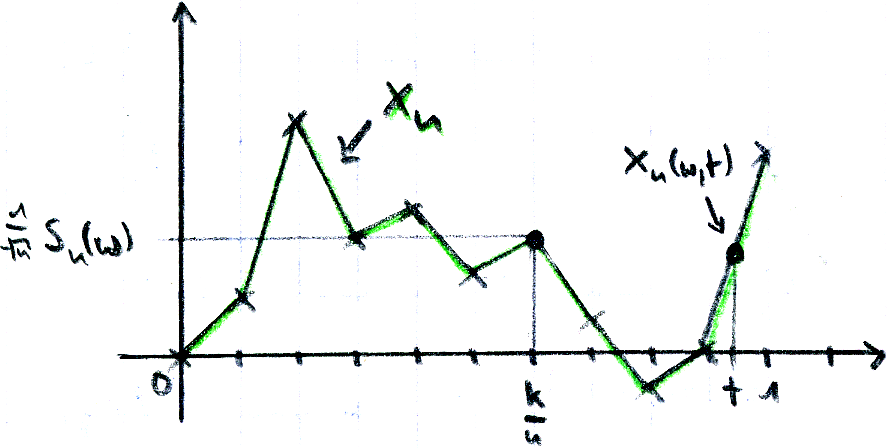
\includegraphics[width=1\textwidth]{./pics/MSTAT001.png}
			\caption{Partialsummenprozess mit $n=10$, $k=6$}
			\label{AbbPartialsummenprozess}
		\end{center}
	\end{figure}
	Mit der Zwei-Punkte-Formel der Geradengleichung folgt:
	\begin{align*}
		X_n(t)
		= \frac{1}{√{n}} \sum_{i=1}^{\floor{nt}} ξ_i + \frac{1}{√{n}} \klammern[\big]{nt-\floor{nt}} · ξ_{\floor{nt} + 1} \qquad ∀ t ∈ \intervall01 = I
	\end{align*}
	Hierbei ist die Gaußklammer (Abrundefunktion) wie folgt definiert:
	\begin{align*}
		\floor u := [u] := \max\set[\big]{l∈\Z : l≤ n}
	\end{align*}
	$X_n(t)$ ist eine reelle Zufallsvariable für alle $t∈ I$.
	Gemäß Konstruktion (Polygonzug) ist jeder Pfad von $X_n$ stetig auf $[0,1]$.
	Aus Satz \ref{satz7.3} folgt, dass $X_n~\A\text{-}\B(C)$-messbar ist, also Zufallsvariable in $\klammern[\Big]{C\klammern[\big]{[0,1]},d}$.

	Weitere Anwendung von Satz \ref{satz7.2}:
\end{beispiel}

\begin{satz}\label{satz7.5}
	\begin{enumerate}[label=(\arabic*)]
		\item \label{it:7.5Masse} $P,Q$ seien Wahrscheinlichkeitsmaße auf $\klammern{C, \B(C)}$. Dann gilt:
			\begin{align*}
				P=Q⇔∀ T⊆ I\text{ endlich}: P∘π_T^{-1}=Q∘π_T^{-1}
			\end{align*}
		\item \label{it:7.5Vars} $X,Y$ seien Zufallsvariablen in $\klammern[\big]{C(I),d}$. Dann gilt:
			\begin{align*}
				X\stackeq{\L}Y⇔∀ T⊆ I\text{ endlich }: π_T(X)\stackeq{\L}π_T(Y)
			\end{align*}
	\end{enumerate}
\end{satz}

\begin{proof}~
	\paragraph{Zu \ref{it:7.5Masse}, zeige \enquote{$⇒$}} Trivial.
	\paragraph{Zu \ref{it:7.5Masse}, zeige \enquote{$⇐$}}
	Gemäß Satz \ref{satz7.2} ist
	\begin{align*}
		\mathcal{E}:=\set{π_T^{-1}(A):A∈\B\argu{ℝ^{\measure{T}}},T⊆ I\text{ endlich}}
	\end{align*}
	ein Erzeuger von $\B(C)$, d.\,h.\ $\B(C)=σ(\mathcal{E})$. Erinnerung:
	\begin{align*}
		g^{-1}(\mathcal{C})&:=\set[\big]{ g^{-1}(C):C∈\mathcal{C}}\text{ für Mengenfamilie }\mathcal{C}\\
		\B(C)&\stackeq{\ref{satz7.2}}σ\argu[\big]{π_T:T⊆ I\text{ endlich}}
		=σ\argu[\Bigg]{\underbrace{
			\Union_{
				\begin{subarray}{c}
					T⊆ I \\
					T\text{ endlich}
				\end{subarray}}
				π_T^{-1} \argu{ \B\argu{ℝ^{\abs{T}}}}
		}_{=\mathcal{E}}}
	\end{align*}
	Nach Voraussetzung gilt:
	\begin{align*}
		P \argu{π_T^{-1}(A)} \overset{\text{Def}}= P∘π_T^{-1}(A)
		&= Q∘π_T^{-1}(A) = Q \argu{π_T^{-1}(A)} \qquad ∀ A ∈ \B \klammern{ℝ^{\abs{T}}}\\
		⇒
		\restr{P}{\mathcal{E}} &= \restr{Q}{\mathcal{E}}
	\end{align*}
	$\mathcal{E}$ ist durchschnittsstabil (nachrechnen!).
	Damit liefert der \undefine{Maßeindeutigkeitssatz}, dass $P=Q$ auf $σ(\mathcal{E})=\B(C)$.
	(Der Maßeindeutigkeitssatz besagt:
	zwei Wahrscheinlichkeitsmaße, die auf einen schnittstabilen Mengensystem überein stimmen, stimmen auch auf dessen Erzeugnis überein.)
	\paragraph{Zeige \ref{it:7.5Vars}}
	\begin{align*}
		X\stackeq{\L} Y
		\overset{\text{Def}}&{⇔}
		\P∘ X^{-1}=\P∘ Y^{-1}\\
		\overset{\ref{it:7.5Masse}}&{⇔}
		\underbrace{\argu{\P∘ X^{-1}}∘ π_T^{-1}}_{=\P∘\klammern{π_T∘ X}^{-1}}
		=\underbrace{\klammern{\P∘ Y^{-1}}∘π_T^{-1}}_{=\P∘\klammern{π_T∘ Y}^{-1}}
		&∀ T⊆ I\text{ endlich}\\
		&⇔
		\underbrace{π_T∘ X}_{=π_T(X)}\stackeq{\L}\underbrace{π_T∘ Y}_{=π_T(Y)}
		&∀ T⊆ I\text{ endlich}
		& \qedhere
	\end{align*}
\end{proof}

\begin{bemerkungnr} %7.6
	Die Wahrscheinlichkeitsmaße $\P∘\klammern[\big]{π_T∘ X}^{-1}$ bzw.\ die Verteilungen
	% CHECKED: 'bzw.' used.
	\begin{align*}
		π_T(X) &= \klammern[\big]{X(t_1), …, X(t_k)} & ∀ & T =\set{t_1,…,t_k} ⊆ I\text{, genauer:}\\
		π_T\argu[\big]{X(ω)} &= \klammern{X(ω)(t_1),…,X(ω)(t_k)} & ∀ & ω∈Ω, ∀ T = \set{ t_1,…,t_k}⊆ I\\
		&π_T∘ X\colonΩ⟶ C⟶ℝ_k
	\end{align*}
	heißen \define{endlich dimensionale Randverteilungen von $\P$} bzw.\ \define{von $X$}.
	% CHECKED: 'bzw.' used.
	Insbesondere ist gemäß \ref{satz7.5} \ref{it:7.5Vars} die Verteilung eines stetigen stochastischen Prozesses $X$ aufgefasst als Zufallsvariable in $C$ eindeutig durch die Verteilungen der Vektoren
	\begin{align*}
		\klammern[\big]{X(t_1),…,X(t_k)},\qquad t_1,…,t_k∈ I,k∈ℕ
	\end{align*}
	festgelegt.
\end{bemerkungnr}


	% !TEX root = MSTAT19.tex
% This work is licensed under the Creative Commons
% Attribution-NonCommercial-ShareAlike 4.0 International License. To view a copy
% of this license, visit http://creativecommons.org/licenses/by-nc-sa/4.0/ or
% send a letter to Creative Commons, PO Box 1866, Mountain View, CA 94042, USA.

Nächstes Ziel: Handhabbare Kriterien für den Nachweis der Verteilungskonvergenz in $C$. Dazu:

\begin{definition} %7.7
	Für eine Funktion $f \colon I ⟶ ℝ$ und $δ > 0$ definiere den \define{Stetigkeitsmodul/ Oszillationsmodul}
	\begin{align*}
		ω(f,δ):=\sup \set[\Big]{\abs{f(s)-f(t)}:s, t ∈ I \mit \abs{s-t} ≤ δ}
	\end{align*}
\end{definition}

Aus der Analysis ist bekannt:
\begin{align*}
	f∈ C(I)⇔ω(f,δ)\overset{δ⟶0}{\longrightarrow}0
\end{align*}

\begin{lemma}\label{lemma7.8}
	$ω(·,δ)\colon (C,d)⟶ℝ$ ist stetig für jedes $δ>0$ und damit gemäß Lemma \ref{Lemma3.2} \ref{it:3.2StetigMessbar} auch $\B(C)$-$\B(ℝ)$-messbar.
\end{lemma}

\begin{proof}
	Sei $g∈ C$ und $s,t∈ I$ mit $\abs{s-t}≤δ$.
	Dann gilt:
	\begin{align*}
		\abs{f(s)-f(t)}
		&= \abs[\big]{f(s)-g(s)+g(s)-g(t)+g(t)-f(t)}\\
		\overset{\text{DU}}&{≤}
		\underbrace{\abs{f(s)-g(s)}}_{≤ d(f,g)}
		+ \underbrace{\abs{g(s)-g(t)}}_{ ≤ ω(g,δ)}
		+ \underbrace{\abs{ g(t)-f(t)}}_{≤ d(f,g)}\\
		& ≤
		ω(g,δ)+2· d(f,g)\\
		\overset{\sup}&{⇒}
		ω(f,δ)
		≤ ω(g,δ) + 2 d(f,g)\\
		&⇒ ω(f,δ)-ω(g,δ)
		≤ 2 d(f,g) %& ∀ f,g
		\\
		&⇒ ω(g,δ) - ω(f,δ)
		≤ 2 d(g,f) = 2 d(f,g)
		\\
		&⇒
		\abs{ω(f,δ)-ω(g,δ)}≤ 2 d(f,g)
	\end{align*}
	Das heißt, $ω(·,δ)$ ist sogar Lipschitz-stetig.
\end{proof}

%Ferger: "Ich war übrigens gestern in der Stadt. Da bin ich eigentlich nie. Ich war in mindestens 7 oder Schuhgeschäften. Es war noch jemand dabei. Ich selber habe kein Schuhe gekauft. Und in jedem Geschäft war die Verweildauer sehr lang. Und jedes Schuhgeschäft wurde GESCANNT: Jeder Schuh wurde angefasst und begutachtet. [...] Weihnachten ist was Schönes!"

%Ferger: "Wenn man sich rote Schuhe kauft, muss man dazu auch noch eine passende rote Tasche kaufen. Wussten Sie das?"

% Dieses Jahr regt sich Ferger über die Rente auf. Die Franzosen protestieren, was er
% prinzipiell richtig findet, aber sich wundert, da die Franzosen bisher mit 62 in Rente gehen
% während er als erster Jahrgang mit 67 in Rente gehen wird.
% Das geht noch eine ganze Weile weiter.
% Schließlich regt er sich über Merz auf, der die SPD eine 11%-Partei genannt hat Ferger dachte, Merz
% sei in der FDP. Aber Merz ist CDU.
% Ferger ist Grünen-Wähler.
Erstes Kriterium für Verteilungskonvergenz in:

\begin{satz}\label{satz7.9}
	Seien $X,X_n,n∈ℕ$ Zufallsvariablen in $C$ über $(Ω,\A,\P)$. Falls
	\begin{enumerate}[label=(\arabic*)]
		\item \label{it:7.9fd}
			$X_n\fdto  X$, das heißt
			\begin{align*}
				 \underbrace{\klammern[\big]{X_n(t_1),…,X_n(t_k)}}_{=π_T∘ X_n} \distrto \underbrace{\klammern[\big]{X(t_1),…,X(t_k)}}_{=π_T∘ X}
				\quad∀ t_1,…,t_k∈ I\,∀ k∈ℕ,
			\end{align*}
			die so genannte \define{Konvergenz der fidis} (finite dimensional distributions, gesprochen \enquote{feidies}).
		\item \label{it:7.9limlimsup}
			$\begin{aligned}
				\lim_{k⟶∞}\limsup_{n⟶∞}\P\klammern[\Big]{ω\klammern[\big]{X_n,δ_k}>ε}=0\qquad∀ε>0
			\end{aligned}$\\
			für eine Folge $(δ_k)_{k∈ℕ}$ in $(0,∞)$ mit $δ_k \downarrow 0$
	\end{enumerate}
	so folgt:
	\begin{align*}
		X_n\distrto X\text{ in }(C,d)
	\end{align*}
\end{satz}
% Dieses Kriterium ist häufig nützlich für Martingale mit Maximalungleichungen.
% In seiner Dissertation hat er sich mit diesem Kriterium und den Stetigkeitsmoduln herumgeplagt.
% Das war schwierig.
\begin{proof}
	Siehe \cite[Seite 348]{gaensslerstute1977Wahrscheinlichkeitstheorie}.
\end{proof}
\begin{proof}[Felix' Beweis]\footnote{Nicht in der Vorlesung behandelt.}
	Laut Portmanteau-Theorem \ref{satz4.2} genügt es für $f \colon C(I) → ℝ$ gleichmäßig stetig
	und beschränkt zu zeigen,
	dass
	\begin{equation} \label{eq:7.9Ziel}
		∫_{C(I)} f \d (\P ∘ X_n^{-1}) → ∫_{C(I)} f \d (\P ∘ X^{-1}).
	\end{equation}
	Mit \ref{it:7.9fd} haben wir diese Konvergenz erstmal nur für spezielle $f$,
	nämlich solche der Form $f = \tilde{f} ∘ π_T$ mit $T ⊂ I$, $T$ endlich,
	mit $\tilde f \colon ℝ^{\measure{T}} → ℝ$ gleichmäßig stetig und beschränkt.

	Um \eqref{eq:7.9Ziel} auf die fidis zurückzuführen, betrachten wir den Fehler,
	den wir machen, wenn wir statt $f$ nur endlich viele Punkte betrachten:
	\begin{equation}
		\text{Sei } \tilde{f}_T (x_1, ..., x_{\measure{T}})
		:= f \argu[\Big]{\operatorname{Poly} \argu[\Big]{ (t_1, x_1), ..., (t_{\measure{T}}, x_{\measure{T}}) }},
	\end{equation}
	wobei $T = \set{t_1, ..., t_{\measure{T}}}$, $\inf I = t_1 < ... < t_{\measure{T}} = \sup I$,
	und $\operatorname{Poly}$ der Polygonzug durch die angegebenen Punkte ist,
	analog zur Konstruktion in Donsker \ref{satz7.9}.
	Für $h ∈ C(I)$ sei $\operatorname{Poly}(h, T)$ der Polygonzug, der als Stützpunkte
	die Elemente von $T$ hat und in diesen mit $h$ übereinstimmt.

	Zu $δ_k$ wähle nun $T_k ⊂ I$ so, dass die Abstände aufeinanderfolgender Punkte
	kleiner ist als $δ_k$ (z.\,B.\ gleichverteilt).

	Dann gilt
	\begin{equation} \label{eq:7.9Polyannaehrung}
		\norm{h - \operatorname{Poly}(h, T_k)}_{∞} ≤ 2 ω(h, δ_k) \quad (h ∈ C(I)).
	\end{equation}
	Dies lässt sich sehen, wenn man sich einen Abschnitt zwischen zwei Elementen
	betrachtet:
	\begin{align*}
		\text{Für } s ∈ \intervall{t_i}{t_{i + 1}}:
	  \abs{h(t_i) - X(s)} &< ω(h, δ_k) \\
		\text{und }
		\abs{h(t_i) - \operatorname{Poly}(h, T_k)(s)} &=
		\abs{\operatorname{Poly}(h, T_k)(t_i) - \operatorname{Poly}(h, T_k)(s)} \\
		&≤ \abs{\operatorname{Poly}(h, T_k)(t_i) - \operatorname{Poly}(h, T_k)(t_{i+1})} \\
		&= \abs{h(t_i) - h(t_{i + 1})} < ω(h, δ_k) \\
		⇒ \abs{h(s) - \operatorname{Poly}(h, T_k)(s)} &< 2 ω(h, δ_k)
	\end{align*}
	%
	Betrachte nun den Fehler durch Diskretisierung für einen stochastischen Prozess $Y \colon Ω → C(I)$
	\begin{align*}
		\abs{ ∫_{C(I)} \tilde f ∘ π_{T_k} - f \, \d (\P ∘ Y^{-1})}
		\overset{Δ\neq}&{≤} ∫_{Ω} \abs{ f(\operatorname{Poly}(Y, δ_k)) - f(Y) } \, \d \P \\
		\overset{\eqref{eq:7.9Polyannaehrung}}&{≤} ∫_{Ω} ω(f, 2 ω(Y, δ_k)) \, \d \P
	\end{align*}
	Da $f$ nach Annahme gleichmäßig stetig und $\P$ ein Wahrscheinlichkeitsmaß ist, ist die rechte Seite endlich. (Die Beträge entfallen, da der Stetigkeitsmodul immer nicht-negativ ist.)

	Diese Abschätzung kann nun für $X_n$ und $X$ genutzt werden:
	\begin{align}
		\abs{ ∫_{Ω} f \d (\P ∘ X_n^{-1}) - ∫_{Ω} f \d (\P ∘ X^{-1}) }
		\overset{Δ\neq}&{≤}
		∫_{Ω} ω(f, 2ω(X_n, δ_k)) \d \P \label{eq:7.9Xnpart} \\
		&\, +
		∫_{Ω} ω(f, 2ω(X, δ_k)) \d \P \label{eq:7.9Xpart} \\
		&\, +
		\klammern{ ∫_{Ω} \tilde f ∘ π_{T_k} ∘ X_n \d \P
		- ∫_{Ω} \tilde f ∘ π_{T_k} ∘ X \d \P } \label{eq:7.9discretePart}
	\end{align}
	Die drei Summanden möchten wir nun nach oben abschätzen. Gebe dafür ein $ε > 0$ vor.

	Betrachte \eqref{eq:7.9Xnpart}. $f$ ist beschränkt nach Voraussetzung, das heißt
	$ω(f, δ) < 2 \norm{f}_{∞}$ für alle $δ$. Wähle nun $η > 0$ so klein, dass
	$ω(f, η) < \frac{ε}{6}$. Dies geht, da $f$ gleichmäßig stetig ist.

	Wähle des weiteren $k_0 ∈ ℕ$ so groß, dass \ref{it:7.9limlimsup} für alle $k ≥ k_0$ liefert:
	$\P(2 ω(X_n, δ_k ≥ η) < \frac{ε}{6 · 2\norm{f}_{∞}}$ für alle $n ≥ n_0$, $n_0 ∈ ℕ$.
	Dann kann das Integral \eqref{eq:7.9Xnpart} aufgespalten werden, falls $k > k_0$:
	\begin{align*}
		∫_{Ω} ω(f, 2ω(X_n, δ_k)) \, \d \P
		& ≤ ∫_{\set{2 ω(X_n, δ_k) < η}} ω(f, 2ω(X_n, δ_k)) \, \d \P \\
		& \phantom{≤} + ∫_{\set{2 ω(X_n, δ_k) ≥ η}} ω(f, 2ω(X_n, δ_k)) \, \d \P \\
		& ≤ 1 · ω(f, η) + \frac{ε}{6 \norm{f}_{∞}} ω(f, 2ω(X_n, δ_k)) \\
		& ≤ \frac{ε}{6} + \frac{ε}{6 · 2 \norm{f}_{∞}} · 2 \norm{f}_{∞} = \frac{ε}{3}
	\end{align*}
	%
	$η$ ergibt auch für \eqref{eq:7.9Xpart} Sinn. Da $X$ ein stetiger stochastischer Prozess
	ist, gilt $ω(X, δ_k) → 0$ für $k → ∞$ (und damit $δ_k → 0$) (nicht nur fast) sicher.
	Damit konvergiert dies auch stochastisch, das heißt, es gibt ein $k_1 ∈ ℕ$, sodass
	für alle $k ≥ k_1$ wir $\P(2ω(X, δ_k) > η) < \frac{ε}{6}$ haben.
	Damit ergibt das gleiche Argument wie für \eqref{eq:7.9Xnpart}, dass \eqref{eq:7.9Xpart}
	kleiner als $\frac{ε}{3}$ ist für $k ≥ k_0$.

	Wegen der Konvergenz der fidis \ref{it:7.9fd} geht für jedes feste $δ_k$ \eqref{eq:7.9discretePart} gegen $0$.
	Wähle also $k_2 = \max \set{k_0, k_1}$ und $n_1 ≥ n_0$ so, dass $\eqref{eq:7.9discretePart} < \frac{ε}{3}$ für alle $n ≥ n_1$.
	Damit ist
	\begin{equation*}
		\abs{ ∫_{Ω} f \d (\P ∘ X_n^{-1}) - ∫_{Ω} f \d (\P ∘ X^{-1}) }
		< \frac{ε}{3} + \frac{ε}{3} + \frac{ε}{3} = ε \quad ∀ n ≥ n_1
	\end{equation*}
	Damit gilt $X_n \distrto X$.
\end{proof}

\begin{beispiel}\label{beispiel7.10} Sei
	\begin{align*}
		X_n(t):=A_n+B_n· t+C_n· t^2\quad∀ t∈ I = \intervall {α}{β}
		\quad\mit \klammern[\big]{A_n,B_n,C_n}\distrto (A,B,C)∈ℝ^3
	\end{align*}
	Dann gilt:
	\begin{align*}
		X_n\ntoinf  X\text{ in }(C,d)\qquad\mit\qquad X(t)=A+B· t+C· t^2
	\end{align*}
	Man sagt: $X_n$ und $X$ sind quadratische Funktionen mit zufälligen Koeffizienten.

	\begin{proof}[1. Beweis] Anwendung von \ref{satz7.9}, zur Übung. Hier der Beweis vom Jahr 2018:

		Seien $t_1,…,t_k∈ I$ beliebig.
		Für Voraussetzung \ref{it:7.9fd} in Satz \ref{satz7.9} reicht es gemäß Cramér-Wold-Device \ref{satz5.4CramerWoldDevice} zu zeigen:
		\begin{align*}
			\sum_{j=1}^k λ_j · X_n(t_j)
			\distrto \sum_{j=1}^n λ_j· X(t_j) \text{ in } ℝ
			\qquad ∀ λ = \klammern[\big]{λ_1,…,λ_k} ∈ ℝ^k
		\end{align*}
		%Ich wurde von Prof Ferger bemitleidet, weil ich in Tex nicht alles umsetzen kann, was er an der Tafel durch Wisch-Technik erzeugt.
		Dazu:
		\begin{align*}
			\sum_{j=1}^kλ_j· X_n(t_j)
			&=A_n·\sum_{j=1}^nλ_j+B_n·\sum_{j=1}^kλ_j· t_j+C_n·\sum_{j=1}^kλ_j· t_j^2\\
			\overset{\L,\ref{satz4.10ContinuousMappingTheorem}}&{\longrightarrow}
			A·\sum_{j=1}^kλ_j+B·\sum_{j=1}^kλ_j· t_j+C·\sum_{j=1}^kλ_j· t_j^2
			=\sum_{j=1}^kλ_j· X(t_j)
		\end{align*}
		Zu Voraussetzung \ref{it:7.9limlimsup} in Satz \ref{satz7.9}:
		\begin{align*}
			\abs{X_n(s)-X_n(t)}
			&=\abs[\Big]{B_n·(s-t)+C_n·\underbrace{\klammern[\big]{s^2-t^2}}_{(s-t)·(s+t)}}\\
			\overset{Δ\neq}&{≤}
			\abs{B_n}·\underbrace{\abs{s-t}}_{≤δ}+\abs{C_n}·\underbrace{\abs{s-t}}_{≤δ}·\underbrace{\abs{s+t}}_{≤\abs{s}+\abs{t}≤:K}\\
			&≤
			\abs{B_n}·δ+K·\abs{C_n}·δ\qquad∀ s,t∈ I\mit \abs{s-t}≤δ\\
			\overset{\sup}{⇒}
			ω(X_n,δ)
			&≤\abs{B_n}·δ+K·\abs{C_n}·δ\\
			⇒
			\P\klammern[\Big]{ω\klammern[\big]{X_n,δ}>ε}
			&≤\P\argu[\Big]{\abs{B_n} · δ + K · \abs{C_n} · δ > ε}\\
			\overset{\eqref{eqProofBeispiel7.10}}&{≤}
			\P\argu[\Big]{\abs{B_n}·δ>\frac{ε}{2}}+\P\argu[\Big]{K·\abs{C_n}·δ>\frac{ε}{2}}\\
			&=
			\P\argu[\Big]{\abs{B_n}>\frac{ε}{2 δ}}+\P\argu[\Big]{\abs{C_n}>\frac{ε}{2 K δ}}\\
			&=
			1-F_n\klammern{\frac{ε}{2 δ}}+1-G_n\klammern{\frac{ε}{2 K δ}}
		\end{align*}
		%Ferger: "Warum habe ich das eigentlich so gemacht!?"
		Hierbei ist $F_n$ die Verteilungsfunktion von $\abs{B_n}$ %\distrto \abs{B}$
		und $G_n$ die Verteilungsfunktion von $\abs{C_n}$.
		Erinnerung:
		\begin{align}\label{eqProofBeispiel7.10}
			\set[\big]{ U+V>ε}⊆\set{ U>\frac{ε}{2}}∪\set{ V>\frac{ε}{2}}
		\end{align}
		Mit Korollar \ref{korollar4.5} folgt, dass es eine Folge $(δ_k)_{k∈ℕ}$  mit $δ_k\downarrow0$,
		so dass $\frac{ε}{2 δ_k}$ und $\frac{ε}{2 K δ_k}$ Stetigkeitsstellen der jeweiligen Grenz-Verteilungfunktionen sind,
		%Ferger: "Na gut, einen Nobelpreis für Literatur kriege ich jetzt nicht."
		\begin{align*}
			\limsup_{n⟶∞} \P\argu[\big]{ω \argu{X_n,δ_k} > ε}
			≤ \P\argu[\Big]{\abs{B} > \underbrace{\frac{ε}{2 δ_k}}_{\overset{k⟶∞}{\longrightarrow}∞}}
			+\P\argu[\Big]{\abs{C} > \underbrace{\frac{ε}{2 K δ_k}}_{\overset{k⟶∞}{\longrightarrow}∞}}
			\qquad∀ k∈ℕ
		\end{align*}
		%Ferger: "Hach ich bin so doof. Ich hätte mir das Leben leichter machen können."
		$k⟶∞$ liefert dann \ref{it:7.9limlimsup}.
	\end{proof}
	\begin{proof}[2. Beweis]
		Sei $h \colon ℝ^3 → C$, $(a, b, c) ↦ h(a, b, c) \colon I → ℝ : t ↦ h(a, b, c)(t) := a + bt + ct^2$.
		$h$ ist stetig auf $ℝ^3$, denn: Sei $(a_n, b_n, c_n) → (a, b, c)$.
		Dann
		\begin{align*}
			d(h(a_n, b_n, c_n), h(a, b, c))
			&= \sup_{t ∈ I} \abs{a_n + b_n + c_n t^2 - (a + bt + c^2)} \\
			&≤ \sup_{t ∈ I} \abs[\big]{a_n - a} + \abs[\big]{(b_n - b) t} + \abs{(c_n - n) t^2} \\
			&≤ \abs{a_n - a} + \abs{b_n - b} L + \abs{c_n -c} L^2 \quad L := \max(\abs{α}, \abs{β}) \\
			&→ 0 + 0 · L + 0 · L^2 = 0
		\end{align*}
		Damit ist $h$ stetig.
		Mit dem CMT \ref{satz4.10ContinuousMappingTheorem} folgt
		wegen der Voraussetzung $(A_n, B_n, C_n) \distrto (A, B, C)$
		\begin{align*}
			X_n = h(A_n, B_n, C_n) \distrto h(A, B, C) = X & \qedhere
		\end{align*}
	\end{proof}
\end{beispiel}

Zweite handlicherere Möglichkeit für den Nachweis der Verteilungskonvergenz in $C$ liefert:

\begin{satz}[Momentenkriterium von Kolmogoroff]\label{satz7.11MomentenkriteriumVonKolmogoroff}\enter
	Seien $X,X_n,n∈ℕ$ Zufallsvariablen in $C$ mit
	\begin{align}\label{eqSatz7.11Vor1}\tag{cfd}
		X_n\fdto  X\qquad\text{(vgl.\ \ref{it:7.9fd} in Satz \ref{satz7.9})}
	\end{align}
	Falls es eine Konstante $γ>0$ und $α>1$ sowie eine stetige und monoton wachsende Funktion $F:I⟶ℝ$ gibt, derart, dass
	\begin{align}\label{eqSatz7.11VorM}\tag{M}
		\Earg[\Big]{\abs{X_n(s)-X_n(t)}^γ} ≤ \klammern[\big]{F(s)-F(t)}^α \qquad ∀ s, t ∈ I \mit s>t
	\end{align}
	(\define{Momentenbedingung}).
	Dann gilt:
	\begin{align*}
		X_n\distrto  X\text{ in }\klammern[\big]{C(I),d}
	\end{align*}
\end{satz}

\begin{proof}
	Siehe \cite[Seite 96]{billingsley2013convergence} % B illingsley (1968), \undefine{Convergence of probability measures}, Seite 96.
	%Ferger: "Das Buch hier war früher meine Fibel."
	%Ferger: "Jim Morrison von den Doors. Das war mein Held. Neben Skorokott."
\end{proof}

\paragraph{Ziel:} Verteilungskonvergenz der Partialsummenprozesse $X_n$ aus dem Beispiel \ref{beispiel7.4}.
Dazu:

\begin{definition}[Brownsche Bewegung] \label{def7.12} %7.12
	Sei $I=[0,b]\mit b>0$ und $B:=\set[\big]{ B(t):=B(t,ω), t ∈ I}$ ein stetiger stochastischer Prozess über $(Ω,\A,\P)$ mit
	\begin{enumerate}[label=(\arabic*)]
		\item \label{it:7.12begin0} $\begin{aligned}
			B(0)=B(0,ω)=0\qquad∀ω∈Ω
		\end{aligned}$
	\item \label{it:7.12independantchanges} $∀\, 0=:t_0≤ t_1<…<t_r≤ b$, $r ∈ ℕ$
		sind die Zuwächse $B(t_i)-B(t_{i-1})$, $1≤ i≤ r$ \emph{unabhängig}
	\item \label{it:7.12normal} $\begin{aligned}
			0≤ s<t≤ b⇒ B(t)-B(s)\sim\mathcal{N}(0,t-s)
		\end{aligned}$
	\end{enumerate}
	Dann heißt $B$ \define{Brownsche Bewegung (BB)} auf $I$.

	Vollkommen analog definiert man eine BB auf $I= ℝ_{+} = [0,∞)$.
\end{definition}

%Ferger: "Das ist wie so ein Wunschzettel. Es gelte 1, 2 und 3. Passend zur Weihnachtszeit. Wenn's dumm läuft, kann es noch sein, dass mein Wunsch nicht erfüllt wird, weil er nicht erfüllt werden kann."
%Ferger: "In der Hoffnung das Sie nicht schonmal hier gesessen haben: Weil ich immer dieselben Geschichten erzähle. Ich bin jetzt in so einem Alter wo man alles mehrfach erzählt."
%Ferger: "Da hat mal jemand eine Doktorarbeit geschrieben über eine tolle Funktionenklasse. Und dann kam jemand daher, dass die Funktionenklasse nur aus der Eins-Funktion besteht. Das war echt ein Griff ins Klo. Wäre noch heftiger gewesen, wenn die Funktionenklasse leer gewesen wäre. Aber: So sind wir ja auch alle gestrickt. So werden wir konditionert. Weil, wenn der Mathematiker irgendwas hört, fragt der Mathematiker ständig "Existiert das?""

\begin{satz}[Lévy]\label{satz7.13Levy}
	Eine Brownsche Bewegung existiert.
\end{satz}

\begin{proof}
	Siehe Vorlesung \undefine{Stochastische Prozesse}.
	%Ferger: "Es gibt einen konstruktiven Beweis, der ist auch lehrrreich, aber da haben wir jetzt keine Zeit für.
	%Anmerkung des Autors: Geschichten erzählen ist wohl wichtiger.
\end{proof}

\begin{lemma}\label{lemma7.14}
	Sei $B$ eine BB auf $I$ und $t_1<…<t_r$ aus $I$. Dann gilt:
	\begin{align*}
		\klammern[\Big]{B(t_1),…, B(t_r)}^T\sim\mathcal{N}_r(0,Γ)\text{ wobei }\\
		Γ:= \klammern[\Big]{\Cov\klammern[\big]{B(t_i),B(t_j)}}_{1≤ i,j≤ r}
	=\klammern[\big]{\min(t_i, t_j)}_{1≤ i,j,≤ r}
	\end{align*}
\end{lemma}

\begin{proof}
	Sei $t_0:=0$. Dann gilt:
	\begin{align*}
		B(t_j)
		\overset{\ref{def7.12}\ref{it:7.12begin0}}=
		B(t_j)-\underbrace{B(t_0)}_{=0}
		\overset{\text{Teles}}{=}
		\sum_{i=1}^j\klammern[\big]{B(t_i)-B(t_{i-1})}
		=\sum_{i=1}^j√{t_i-t_{i-1}}·\underbrace{\frac{B(t_i)-B(t_{i-1})}{√{t_i-t_{i-1}}}}_{=:Z_i}
	\end{align*}
	Da $B(t_i)-B(t_{i-1})\sim\mathcal{N}(0,t_i-t_{i-1})$ folgt, dass die $Z_i$ \iid\ $\sim\mathcal{N}(0,1)$ sind.
	Also ist der Vektor
	\begin{align*}
		\begin{pmatrix}
			B(t_1)\\
			\vdots\\
			B(t_r)
		\end{pmatrix}&=\begin{pmatrix}
			√{t_1} & 0 & \hdots & \hdots & 0\\
			√{t_1} & √{t_2-t_1} & 0 & \hdots & 0\\
			\vdots & \vdots & \ddots & \ddots & \vdots\\
			√{t_1} & √{t_2-t_1} & √{t_3-t_2} & \hdots & √{t_r - t_{r - 1}} \\
			% TOCHECK in der Vorlesung: sollte rechts unten nicht √{t_r - t_{r - 1}} statt 0 stehen?
		\end{pmatrix} \begin{pmatrix}
			Z_1\\
			\vdots\\
			Z_r
		\end{pmatrix} \\ ⇒\begin{pmatrix}
			B(t_1)\\
			\vdots\\
			B(t_r)
		\end{pmatrix} & \sim \mathcal{N}_r(μ,Γ) \quad \text{Def.\ normaler Vektor} \\
		μ_i &:= \Earg[\Big]{B(t_i)}
		= \Earg[\Big]{ \underbrace{B(t_i) - B(t_0)}_{\sim \mathcal{N}(0, t_i - t_0)} } \qquad ∀ i \\
		⇒ μ_i &:= \klammern[\big]{μ_1,…,μ_r}=0
	\end{align*}
	Ferner sei $i≤ j$. Dann gilt:
	\begin{align*}
		\Cov\klammern[\big]{B(t_i),B(t_j)}
		&=\Earg[\Big]{B(t_i)· B(t_j)}\\
		&=\Earg[\Big]{B(t_i)·\klammern[\big]{ B(t_j)-B(t_i)+B(t_i)}}\\
		&=\Earg{B(t_i)·\klammern[\big]{B(t_j)-B(t_i)} + \klammern[\big]{B(t_i)}^2} \\
		&=\Earg[\big]{\underbrace{B(t_i)·\klammern[\big]{B(t_j)-B(t_i)}}_{\text{beide Faktoren sind unabh.}}}
		+\Earg{\klammern[\big]{B(t_i)}^2}\\
		\overset{\text{unab}}&=
		\underbrace{\Earg[\big]{B(t_i)}}_{=0}
		· \underbrace{\Earg[\big]{B(t_j)-B(t_i)}}_{=0}
		+ \underbrace{\Earg[\Big]{\klammern[\big]{B(t_i)}^2}}_{= \Var \argu[\big]{B(t_i)}} \\
		\overset{\text{Vert}}&=
		\Var\klammern[\big]{\mathcal{N}(0,t_i)}\\
		&=t_i\\
		\overset{i≤ j}&{=}
		\min(t_i, t_j)
	\end{align*}
	Analog behandle den Fall $i≥ j$.
\end{proof}

\begin{korollar}\label{korollar7.15Folgerung}
	Die Verteilung einer BB ist eindeutig bestimmt.
\end{korollar}

\begin{proof}
	Seien $B$ und $\tilde{B}$ zwei BBs (i.\,d.\,R.\ über unterschiedlichen Wahrscheinlichkeitsräumen definiert). Dann gilt:
	\begin{align*}
		B \stackeq{\L} \tilde{B}
		\overset{\ref{satz7.5}}&{⇔}
		% todo: uncomment. Attention: wrong utf8-sequence
		\klammern[\big]{B(t_1), …, B(t_r)}^T
		\stackeq{\L}\klammern{\tilde{B}(t_1), …, \tilde{B}(t_r)}^T
		& ∀ t_1 < … < t_r ∈ I, ∀ r ∈ ℕ\\
		\overset{\ref{lemma7.14}}&{⇔}
		\mathcal{N}_r(0,Γ)=\mathcal{N}_r(0,Γ)
		&∀ t_1 < … < t_r ∈ I, ∀ r ∈ ℕ
	\end{align*}
	Die letzte Aussage gilt aber, weil jede mehrdimensionale Normalverteilung $\mathcal{N}_r(μ,Γ)$ eindeutig durch $μ$ und $Γ$ festgelegt ist:
	\begin{align*}
		\mathcal{N}(μ,σ^2)=\mathcal{N}(m,s^2)⇔ m=μ\text{ und }s^2=σ^2
		&
		\qedhere
	\end{align*}
\end{proof}

Die Verteilung $\P∘ B^{-1}=:W$ von  einer Brownschen Bewegung $B$ heißt \define{Wiener-Maß} (nach Norbert Wiener).
%Ferger: "Absoluter Schlaukopf. Ein Ammi. Ein US-Amerikaner. Der hat 21 promoviert. Da wo wir noch mit den Klötzchen spielen, hat der schon promoviert."
\begin{align*}
	B:(Ω,\A,\P)⟶\klammern[\Big]{C(I),\B_d\klammern[\big]{C(I)}}
\end{align*}
%Ferger: "Die Brownsche Bewegung wird genannt Brownsche Bewegeung, weil folgendes passiert ist:
% es gab einen schottischen Bonatiker.
% Der hat also eine Flüssigkeit genommen,
% z.\,B.\ Wasser und dann ganz kleine Pollenkörner oder Staubkörnchen,
% also so was ganz klitzekleines oder eie kleine Minischuppe in sein Töpfchen getan,
% in seine Flüssigkeit und hat draufgeguckt und gesagt "Boah, da ist ja was los." [...]
% Ja ich erzähl das so wie bei der Sendung mit der Maus, weil man das so gut versteht. [...]
% Und er stellt fest, dass da viel los ist.
% Die Beobachtung hatten andere Leute wohl auch schon gemacht.
% Die ersten Leute, jeder von denen hat sich natürlich gefragt: Was steckt dahinter
% Die ersten Leute haben als erklärungsversuch gegeben, dass es biologische Energie in sich hat.
% Der Robert Braun hat gesagt: Nein, das ist nicht so. Können Sie ja mal googeln.
% Entscheidend ist Folgendes: Das war ca. 182?.
% Dann kam Albert Einstein und hat gesagt: Nenene bzw.\ jajaja, was hier passiert ist Folgendes:
% So eine Flüssigkeit besteht ja aus ganz vielen Molekülen, die in Bewegung sind.
% Und die schießen wie wild hin und her. Die Moleküle sind aber klitzeklitzeklein.
% Das kleine Teilchen ist aber im mikroskopischen Bereich,
% also im Vergleich zu den Molekülen ein Riesen-Oschi.
% Und die kleinen Teilchen hauen die ganze Zeit dagegen.
% Der Einstein ist hergegangen und hat das für Physiker-Verhältnisse sehr mathematisch beschrieben.
% Der Wiener hat das nochmal auf saubere, mathematische Füße gestellt
% (Funtionenraum, Verteilungen und solche Sachen...)
% Die haben das ein oder andere wohl handwaving gemacht und
% Norbert Wiener hat das dann mal mathematisch sauber gemacht.
% Deshalb heißt die Verteilung einer Brownschen auch Wiener Maß.

% Ferger: Sind ja immernoch 7 Minuten. Mist. Na da kann ich ja noch eine Geschichte erzählen.

% !TEX root = MSTAT19.tex
% This work is licensed under the Creative Commons
% Attribution-NonCommercial-ShareAlike 4.0 International License. To view a copy
% of this license, visit http://creativecommons.org/licenses/by-nc-sa/4.0/ or
% send a letter to Creative Commons, PO Box 1866, Mountain View, CA 94042, USA.

\begin{satz}[Donsker]\label{satz7.16Donsker}%\enter
	Seien $(ξ)_{i∈ℕ}$ \iid\ mit $\Earg{ξ_1}=0$ und $\Var(ξ_1)=1$.
	\begin{align*}
		S_k &:= \sum_{i=1}^k ξ_i & ∀ & k ∈ ℕ_0 \\
		X_n(t) &:= \frac{1}{√{n}} S_{\floor{n t}}
		+ \frac{1}{√{n}} \klammern[\big]{n t - \floor{n t}} ξ_{\floor{n t} + 1} & ∀ & t ∈ I = \intervall{[0}{b}
	\end{align*}
	($b>0$ fest), d.\,h.\ $X_n$ ist der Polygonzug durch die Punkte $\klammern{\frac{k}{n}, \frac{1}{√{n}} S_k}_{0 ≤ k ≤ bn}$. Dann gilt:
	\begin{align*}
		X_n\distrto  B\text{ in }\klammern[\big]{C(I),d}
	\end{align*}
	wobei $B$ eine BB auf $I=[0,b]$ ist.
\end{satz}
% Vielleicht erzähle ich doch die Geschichte.
% Der Donsker hat die Geschichte 1952 gemacht. Motiviert durch eine andere Arbeit von 1949
% von Duqe (oder so ähnlich). Der hat da ausgerechnet, was die Verteilung des Funktionals
% Brownsche Brücke
% \sup_{0 ≤ t ≤ 1} \abs{B(t)} ist. Wird Ferger uns auch noch zeigen.
% Dann haben Leute wie Kolmogoroff oder Smirnoff sich
% \sup_{0 ≤ t ≤ 1} √n \abs{F_n(t) - F(t)}
% angeschaut und für jedes feste n die Verteilungsfunktion H_n ausgerechnet
% und gesehen, dass dieses schwach gegen eine Verteilung H konvergiert.
% Duqe bemerkt dann seine Verteilung genau dieses H ist.
% Die Vermutung war dann, dass die stochastischen Prozesse auch in irgendeiner Form konvergieren.
\begin{proof}
	Anwendung von Satz \ref{satz7.11MomentenkriteriumVonKolmogoroff}.
	Zeige also dessen Voraussetzungen:
	\paragraph{Zeige Konvergenz der fidis \eqref{eqSatz7.11Vor1}:}
	Seien $0 = t_0 ≤ t_1<…<t_r≤ b$.
	Um den Satz \ref{satz4.14Cramer} von Cramér zu nutzen, betrachte:
	\begin{align*}
		% \norm{\klammern[\big]{X_n(t_i)}_{1≤ i≤ r}-\left(\frac{1}{√{n}}·\sum_{j=1}^{\floor{n· t_i}}ξ_j\right)_{1≤ i≤ r}}
		\norm{\klammern[\big]{X_n(t_i)}_{1≤ i≤ r}
			-\klammern{\frac{1}{√{n}}S_{\floor{nt_i}}}_{1≤ i≤ r}
		}
		% &=\Bigg(\sum_{i=1}^r\underbrace{\left|X_n(t_i)-\frac{1}{√{n}}·\sum_{j=1}^{\floor{n t_i}}ξ_j\right|^2}_{\frac{1}{√{n}}·\underbrace{\big|n· t_i-\floor{n t_i}\big|}_{≤1}·ξ_{\floor{n t_i}}}\Bigg)^{\frac{1}{2}}\\
		&=\klammern[\Bigg]{
			\sum_{i=1}^r
				\underbrace {\abs{X_n(t_i)-\frac{1}{√{n}} S_{\floor{nt_i}}}^2}
				_{ \frac1{√n} \abs[\Big]{
					\underbrace {(n t_i - \floor{n t_i})}
						_{≤ 1}
					ξ_{\floor{n t_i} + 1}
				}
				}
		}^{\frac{1}{2}}\\
		&≤
		\frac1{√n} \klammern{\sum_{i=1}^r ξ_{\floor{n t_i} + 1}^2}^{\frac12}
		% \\⇒
		% \P\klammern{\norm{\klammern[\big]{X_n(t_i)}_{1 ≤ i ≤ r} - \klammern{\frac{1}{√{n}} \sum_{j=1}^{\floor{n t_i}} ξ_j}_{1≤ i≤ r}}}
		% &≤ \P \argu{\sum_{i=1}^r ξ_{\floor{n t_i} + 1}^2 > n ε^2}\\
		% \overset{\text{Markov}}&{≤}
		% \frac1n ε^{-2} \sum_{i=1}^r\underbrace{\Earg{ξ^2_{\floor{n t_i} + 1}}}_{=1~∀ i}\\
		% &=
		% \frac1n ε^{-2} r\ntoinf 0 \qquad ∀ ε > 0 \\
		% ⇒ \norm{(...) - (...)} &≤
		% \frac 1{√n} \klammern{\sum_{i = 1}^r ξ_{\floor{n t_i} + 1} ^2}^{\frac 12}
		\\
		⇒ \P( \norm{...} > ε)
		&≤ \P\argu{ (...)^{\frac 12} > ε √n} %\\
		%&
		= \P\argu{\sum_{i = 1}^r ξ_{\floor{nt_i} + 1} ^2 > ε^2 n} \\
		\overset{\text{Markov}\neq}&{≤}
		\frac 1n ε^{-2} \Earg{\sum_{i = 1}^r ξ^2_{\floor{n t_i} + 1}} \\
		&= \frac 1n ε^{-2} r \ntoinf 0 \quad
		∀\, ε > 0
	\end{align*}
	% $⇒ \klammern[\big]{X_n(t_i)}_{1 ≤ i ≤ r}$ und $\klammern{\frac 1{√n} S_{\floor{n t_i}}}_{1 ≤ i ≤ r}$ sind stochastisch äquivalent. Wegen \ref{satz4.14Cramer} reicht es zu zeigen:
	% \begin{align*} \tag{$*$} % do not know if we use this somewhere
	% 	\klammern{\frac 1{√n} S_{\floor{n t_i}}}_{1 ≤ i ≤ r}
	% 	&\distrto \klammern{B(t_1), ..., B(t_r)} \text{ in } ℝ^r \\
	% 	\overset{\text{CMT} \ref{satz4.10ContinuousMappingTheorem}}{⇔}
	% 	\frac 1{√n} \klammern[\big]{S_{\floor{n t_i}} - S_{\floor{n t_{i-1}}}}_{1 ≤ i ≤ r}
	% 	&\distrto \klammern[\big]{B_{t_i} - B_{t_{i-1}}}_{1 ≤ i ≤ r} \text{ in } ℝ^r
	% \end{align*}
	% denn: $h \colon ℝ^r → ℝ^r$ mit $h(x_1, ..., x_r) = (x_1, x_2-x_1, x_3- x_2, ..., x_r - x_{r-1})$
	% ist stetig auf $ℝ^r$ mit Inverse ... s. unten
  %
	Folglich sind die beiden Folgen
	\begin{align*}
		\klammern[\big]{X_n(t_i)}_{1 ≤ i ≤ r} \qquad \text{und} \qquad
		\klammern{\frac1{√n} \sum_{j=1}^{\floor{n t_i}} ξ_j}_{1≤ i≤ r}
	\end{align*}
	stochastisch äquivalent.
	Wegen Cramér (Satz \ref{satz4.14Cramer}) genügt es
	\begin{align}\label{eqProof7.16fd}\tag{fd}
		\klammern{ \frac1{√n} S_{\floor{n t_i}}}_{1≤ i≤ r}
		\distrto \klammern[\big]{B(t_1),…,B(t_r)}
	\end{align}
	zu zeigen.
	Aber \eqref{eqProof7.16fd} ist äquivalent zu
	\begin{align}\label{eqProof7.16Stern}\tag{$\ast$}
		\frac1{√n} \klammern{S_{\floor{n t_i}} - S_{\floor{n t_{i-1}}}}_{1≤ i≤ r}
		\distrto \klammern[\big]{B(t_i)-B(t_{i-1})}_{1 ≤ i ≤ r}
	\end{align}
	denn:
	\begin{align*}
		h \colon ℝ^r ⟶ ℝ^r, \qquad
		h(x_1,…,x_r) := \klammern{x_1, x_2 - x_1, x_3 - x_2, … , x_r - x_{r-1}}
	\end{align*}
	ist stetig auf $ℝ^r$ und hat stetige Inverse $h^{-1}$ mit
	\begin{align*}
		h^{-1}(y_1,…,y_r) = \klammern{y_1, y_1 + y_2, …, y_1 + … + y_r}
	\end{align*}
	Also ist \eqref{eqProof7.16fd} äquivalent zu \eqref{eqProof7.16Stern} gemäß CMT \ref{satz4.10ContinuousMappingTheorem}.

	Beachte wegen \undefine{Blockungslemma}\footnote{%
		Erläuterung von Felix:
		Die Zuwächse $\frac1{√n} \klammern{S_{\floor{n t_i}}-S_{\floor{n t_{i-1}}}}_{1≤ i≤ r}$
		sind Summen von disjunkten Teilmengen von den $(ξ_k)_k$.
		Die $(ξ_k)_k$ sind unabhängig, damit mit dem Blockungslemma auch die
		Tupel aus mehreren $ξ_{\floor{n t_{i-1}}}$ bis $ξ_{\floor{n t_i}}$
		und damit auch die Summen, da Summenbildung eine messbare Abbildung von
		$ℝ^{\floor{n t_{i - 1}} - \floor{n t_i}}$ nach $ℝ$ ist.
	}
		sind die Zuwächse
	$\frac1{√n} \klammern{S_{\floor{n t_i}}-S_{\floor{n t_{i-1}}}}_{1≤ i≤ r}$ \emph{unabhängig}
	und gemäß \ref{def7.12} \ref{it:7.12independantchanges} sind auch
	$\klammern[\big]{B(t_i)-B(t_{i-1})}$, $1 ≤ i ≤ r$ unabhängig.
	Somit ist gemäß Satz \ref{satz4.21} \eqref{eqProof7.16Stern} äquivalent zu
	\begin{align}\label{eqProof7.16SternStern}\tag{$\ast\ast$}
		\frac1{√n} \klammern{S_{\floor{n t_i}}-S_{\floor{n t_{i-1}}}}
		\distrto
		\klammern[\big]{B(t_i) - B(t_{i-1})} \text{ in } ℝ \qquad ∀ 1 ≤ i ≤ r
	\end{align}
	Dazu setze $k_n:=\floor{n t_i} - \floor{n t_{i-1}}$. Dann gilt:
	\begin{align*}
		&\frac1{√n} \klammern{S_{\floor{n t_i}}-S_{\floor{n t_{i-1}}}}\\
		&=\frac1{√n} \sum_{j=\floor{n t_{i-1}} + 1}^{\floor{n t_i}}ξ_j
		=\frac1{√n} \sum_{j=1}^{k_n}ξ_{\floor{n t_{i-1}} + j}
		\overset{\L}{=}
		\frac1{√n} \sum_{j=1}^{k_n} ξ_j\\
		&= %\underbrace{
		√{\frac{k_n}{n}} %}_{=√{\frac{\floor{n t_i} - \floor{n t_{i-1}}}{n}}}
		· \frac{1}{√{k_n}} \sum_{j=1}^{k_n}ξ_j\\
		&= \underbrace{√{\frac{\floor{n t_i} - \floor{n t_{i-1}}}{n}}}_{\ntoinf √{t_i-t_{i-1}}}
		· \underbrace{\frac1{√{k_n}} \sum_{j=1}^{k_n} ξ_j}_{
				\stackrelnew{\text{ZGWS}}{n⟶∞}{\longrightarrow}
				\mathcal{N}(0,1)}
			\stackrelnew{\ref{beisp4.18} \ref{it:4.18einDim}}{\L}{\longrightarrow}
			√{t_i-t_{i-1}} \mathcal{N}(0,1)
			\overset{\L}{=} \underbrace{\mathcal{N}(0,t_i-t_{i-1})}_{
				\overset{\ref{def7.12}}{=}B(t_i)-B(t_{i-1})}
	\end{align*}
	Damit ist Voraussetzung \eqref{eqSatz7.11Vor1} aus \ref{lemma7.14} gezeigt.

	\paragraph{Momentenbedingung} Wir zeigen \eqref{eqSatz7.11VorM} für $γ=4$ und $α=2$, \emph{falls} $μ_4:=\Earg[\big]{ξ_1^4}<∞$ (das ist eine stärkere Voraussetzung!)

	Seien $s>t$ aus $I = \intervall0b$.
	Dann gilt:
	\begin{equation}\label{eqProof7.16Plus}\tag{+}
		X_n(s) - X_n(t)
		= \frac1{√n} \sum_{j = \floor{n t} + 1}^{\floor{n s}} ξ_j
		+ \frac1{√n} \klammern{n s - \floor{n s}} ξ_{\floor{n s}+1}
		- \frac1{√n} \klammern{n t - \floor{n t}} ξ_{\floor{n t}+1}
	\end{equation}
	Da
	\begin{align}\label{eqProof7.16PlusPlus}\tag{++}
		\floor{n t} ≤ n t < \floor{n t} + 1 \qquad ∀ t ≥ 0
	\end{align}
	folgt für
	\begin{align*}
		k := \floor{n t} \und l := \floor{n s}: \qquad
		\frac kn ≤ t < \frac{k+1}n \und
		\frac ln ≤ s < \frac{l+1}n
	\end{align*}
	\paragraph{Fall 1: $s - t ≤ \frac1n$}
	\begin{enumerate}[label=(\roman*)]
		\item \label{it:7.16proof1} $s$ und $t$ liegen im selben Intervall $\intervallHO{\frac kn}{\frac{k+1}n}$
		\item \label{it:7.16proof2} $s$ und $t$ liegen in benachbarten Intervallen
			$t ∈ \intervallHO{\frac kn}{\frac{k + 1}n}$,
			$s ∈ \intervallHO{\frac{k + 1}n}{\frac{k+2}n}$
	\end{enumerate}
	%Ferger: Habe ich schon erwähnt, dass ich in Deutsch richtig schlecht war?
	\subparagraph{Fall \ref{it:7.16proof1}:} $l = \floor{n s} = \floor{n t} = k$ und
	\begin{align*}
		X_n(s)-X_n(t)
		&=\frac1{√n} (n  s - n t) ξ_{\floor{n t}+1}
		=√n (s - t) ξ_{\floor{n t} + 1} \\
		⇒
		\Earg{\abs[\big]{X_n(s)-X_n(t)}^4}
		&=n^2·(s-t)^4·μ_4
		=μ_4·(s-t)^2·\underbrace{(s-t)^2}_{<\frac{1}{n^2}}· n^2\\
		&≤μ_4·(s-t)^2
	\end{align*}
%Ferger: Sie haben vielleicht mitbekommen es wird momentan von der Digitalisierung geredet. Und der Bund will 5 mrd € zur Verfügung stellen. Aber die Lehrer sagen: "Wir müssen die Kinder in das Zeitalter der Digitalisierung bringen". Gestern, ich lag gerade so auf meiner Couch mit einem Glas Wein und ein Journalist sagte dann "Man darf nicht zurück in die Kreidezeit (Lehrer an der Tafel)" Ich bin so kurz zusammengezuckt und habe mir gedacht: "Ach du scheiße, was machst du denn in Dresden..." Also es gibt tatsächlich Leite, die sich auch damit beschäftigen und sagen das ist Mühsam mit der Tafel. Aber indem man schreibt, beschäftigt man sich schon intensiver mit Stoff.
%Ferger: Manchmal ist weniger mehr.
	\subparagraph{Fall \ref{it:7.16proof2}:} $k=\floor{n t}$ und $l=k+1=\floor{n s}$. Dann folgt aus \eqref{eqProof7.16Plus}:
	\begin{align*}
		X_n(s)-X_n(t)
		&=\frac1{√n} ξ_{k+1}
		+ \frac1{√n} \klammern[\big]{n s - (k+1)} ξ_{k+2}
		- \frac1{√n} (n t - k) ξ_{k+1} \\
		&=√n \klammern{s -\frac{k+1}n} ξ_{k+2}
		+ √n \klammern{\frac{k+1}{n} - t} ξ_{k+1}
	\end{align*}

	\begin{lem}[$c_r$-Ungleichung]
		Seien $a_1, …, a_m ∈ ℝ$ (paarweise verschieden) und $r ≥ 1$. Dann gilt:
		\begin{align}\label{eqCrUngleichung}\tag{$c_r$}
			\abs{\sum_{i=1}^m a_i}^r ≤ c_r \sum_{i=1}^m \abs{a_i}^r \mit c_r := m^{r-1}
		\end{align}
	\end{lem}

	\begin{proof}
		Sei $Z$ diskrete Zufallsvariable mit $\P(Z=a_i)=\frac{1}{m}$ für $1≤ i≤ m$. Dann gilt:
		\begin{align*}
			\abs{\frac1m \sum_{i=1}^m a_i}^r = \abs[\Big]{\Earg{Z}}^r
			\overset{\text{Jensen}} &{≤}
			\Earg[\big]{\abs{Z}^r}
			= \frac{1}{m} \sum_{i=1}^m\abs{a_i}^r
			⇒
			\abs{\sum_{i=1}^m a_i}^r
			≤ m^{r - 1} \sum_{i=1}^m \abs{a_i}^r
			\qedhere
		\end{align*}
	\end{proof}

	Mit $m=2$ und $r=4$ folgt:
	\begin{align*}
		\abs{X_n(s)-X_n(t)}^4
		&≤ 8 \klammern[\bigg]{n^2 ξ^4_{k+2} \klammern[\Big]{\underbrace{s - \frac{k+1}n}_{≤ s - t}}^4
		+n^2 ξ^4_{k+1} \klammern[\Big]{\underbrace{\frac{k+1}n - t}_{≤ s - t}}^4}\\
		⇒
		\Earg{\abs[\big]{X_n(s) - X_n(t)}^4}
		&≤ 16 μ_4 \underbrace{n^2·(s-t)^2}_{≤ 1 ~ \text{(Fall 1)}} (s-t)^2
		≤
		16μ_4 (s-t)^2
	\end{align*}

	\paragraph{Fall 2: $s-t≥\frac1n$}
	Aus \eqref{eqProof7.16Plus} und \eqref{eqCrUngleichung} mit $r=4$ und $m=3$ folgt wegen $\abs[\big]{n s - \floor{n s}} < 1$ und $\abs[\big]{n t - \floor{n t}} < 1$:
	\begin{align} \label{eq:7.16proof2} \tag{$*$}
		\Earg{\abs[\big]{X_n(s)-X_n(t)}^4}
		\overset{}&{≤}
		27 \klammern{\frac1{n^2} \Earg{\abs{\sum_{i = \floor{n t} + 1}^{\floor{n s}} ξ_i}^4}
		+ \underbrace{\frac1{n^2}}_{≤ (s - t)^2} μ_4
		+ \underbrace{\frac1{n^2}}_{≤ (s - t)^2} μ_4}
		\\
		&=
		27 \klammern{\frac1{n^2} \Earg{\abs{\sum_{i = 1 }^{\floor{n s} - \floor{n t}} ξ_{\floor{n t} + 1}}^4}
			+ 2 (s - t)^2 μ_4
		}
	\end{align}

	\begin{lem}[Momentenungleichung]
		Seien $ξ_1,…,ξ_n$ \iid, zentriert mit $μ_2 := \Earg{ξ_1^2}$ und $μ_4 := \Earg{ξ_1^4} < ∞$.
		Dann gilt:
		\begin{align*}
			\Earg{\abs{\sum_{i=1}^nξ_i}^4} = nμ_4 + 3n(n-1)μ_2^2
			≤ 4 μ_4 n^2
		\end{align*}
	\end{lem}

	\begin{proof}[Induktionsbeweis vom zweiten Jahr]
		Sei $S_n := \sum_{i = 1}^{n} ξ_i$. Dann $S_{n + 1} = S_n + ξ_{n + 1}$,
		wobei $S_n$ und $ξ_{n + 1}$ unabhängig sind.
		Zeige die Gleichheit per Induktion nach $n$.

		Der Fall $n = 1$ ist trivial.
		Induktionsschritt:
		\begin{align*}
			\Earg{\abs{S_{n + 1}}^4}
			&= \Earg{(S_n + ξ_{n + 1})^4} \\
			&= \Earg{S_n^4} + 3 \Earg{S_n^3 ξ_{n + 1}}
			+ 6 \Earg{S_n^2 ξ_{n + 1}^2} + 3 \Earg{S_n ξ_{n + 1}^3}
			+ \Earg{ξ_{n + 1}^4} \\
			&= \Earg{S_n^4} + 3 \Earg{S_n^3} \underbrace{\Earg{ξ_{n + 1}}}_{= 0}
			+ 6 \underbrace{\Earg{S_n^2}}_{=n μ_2}  \underbrace{\Earg{ξ_{n + 1}^2}}_{= μ_2}
			+ 3 \underbrace{\Earg{S_n}}_{ = 0} \Earg{ξ_{n + 1}^3}
			+ \underbrace{\Earg{ξ_{n + 1}^4}}_{= μ_4} \\
			\overset{\text{IV}}&{=}
			n μ_4 + 3n(n - 1) μ_2^2 + nμ_2 μ_2 + μ_4
			= (n + 1)μ_4 + 3n(n - 1 + 1) μ_2^2 \\
			&= (n + 1)μ_4 + 3n((n + 1) - 1) μ_2^2
		\end{align*}
		Zur Ungleichung:
		\begin{align*}
			% nμ_4 + 6μ_2^2 \binom n2 = nμ_4 + 6μ_2^2 \frac{n(n - 1)}{2} \\
			\underbrace{n}_{≤ n^2} μ_4
				+ 3 n \underbrace{(n-1)}_{≤ n} \underbrace{μ_2^2}_{=\klammern[\big]{\Earg{ξ_1^2}}^2\overset{\text{Jensen}}{≤} μ_4}
				≤ 4 n^2 μ_4 & \qedhere
	% 	μ_2^2 = (\Earg{ξ_1^2})^2
		% 	\overset{\text{Jensen}}{≤}
		% 	\Earg{ξ_1^4} = μ_4
		% 	⇒ n
		\end{align*}
	\end{proof}
	\begin{proof}[Beweis vom ersten Jahr]

		Zeige zuerst das Gleichheitszeichen:
		\begin{align*}
			\Earg{\abs{\sum_{i=1}^n ξ_i}^4}
			&=\Earg{\klammern{\sum_{i=1}^nξ_i}^4}\\
			&=\Earg{\sum_{1 ≤ i,j,k,l ≤ n} ξ_i·ξ_j·ξ_k·ξ_l} \\
			&=\sum_{1 ≤ i,j,k,l ≤ n} \underbrace{\Earg[\Big]{ξ_i·ξ_j·ξ_k·ξ_l}}_{=: μ_{i,j,k,l}}
		\end{align*}
		Die Tupel $(i,j,k,l)∈\set{1,…,n}^4$ mit mindestens drei verschiedenen Komponenten liefern $μ_{i,j,k,l}=0$,
		denn z.\,B.\ (verschiedene Buchstaben repräsentieren verschiedene Zahlen):
		\begin{align*}
			μ_{i,j,k,j}
			&=\Earg[\Big]{ξ_i·ξ_j·ξ_k·ξ_j}
			=\Earg[\Big]{ξ_i·ξ_j^2·ξ_k}
			=\underbrace{\Earg[\big]{ξ_i}}_{=0} · \Earg[\big]{ξ_i^2} \Earg[\big]{ξ_k}
		\end{align*}
		Folglich reduziert sich die obige auf (!)
		\begin{align*}
			&\sum_{i=1}^4 \underbrace{\Earg[\Big]{ξ_i^4}}_{=μ_4}
			+ 6 \sum_{1 ≤ i ≤ j ≤ n}
			\underbrace{\Earg[\Big]{ξ_i^2 ξ_j^2}}_{=μ_2^2}
			+\underbrace{
				16 \sum_{1 ≤ i ≤ j ≤ n}
					\underbrace{\Earg[\Big]{ξ_i}}_{=0}
					\Earg[\Big]{ξ_j^3}
				+ 4 \sum_{1 ≤ i ≤ j ≤ n}
					\Earg[\Big]{ξ_i^3}
					· \underbrace{\Earg[\Big]{ξ_j}}_{=0}
			}_{=0} \\
			&= nμ_4 + 6μ_2^2 \binom n2 = nμ_4 + 6μ_2^2 \frac{n(n - 1)}{2} \\
			&= \underbrace{n}_{≤ n^2} μ_4
				+ 3 n \underbrace{(n-1)}_{≤ n} \underbrace{μ_2^2}_{=\klammern[\big]{\Earg{ξ_1^2}}^2\overset{\text{Jensen}}{≤} μ_4}\\
			&≤ 4 n^2 μ_4
		\end{align*}
		Siehe auch \cite{ferger2014moment} %\undefine{Turkish Journal of Mathematics, Moment equalities via integer partitions} (2014) von Dietmar Ferger
		für mehr Hintergründe.
	\end{proof}

	Mit diesem Lemma folgt:
	\begin{align*}
		% \frac1{n^2} \Earg{\abs{\sum_{i = \floor{n t}+1}^{\floor{n s}} ξ_i}^4}
		% &=
		\frac1{n^2} \Earg{\abs{\sum_{i=1}^{\floor{n s} - \floor{n t}} ξ_{i + \floor{n t}}}^4}
		%\\
		% &≤ \frac4{n^2} μ_4
		% 	\klammern[\Big]{\underbrace{\floor{n s}-\overbrace{\floor{n t}}^{>n· t-1}}_{≤\underbrace{ n· s-n· t}_{=n·(s-t)}+\underbrace{1}_{\overset{\text{2. Fall}}{≤}n·(s-t)}≤2· n·(s-t)}}^2\\
		% CHECKED: '\Big' used.
		&≤ \frac4{n^2} μ_4 \klammern[\big]{\floor{n s} - \floor{n t}}^2 \\
		&= \frac4{n^2} μ_4 \klammern{n s - n t + (nt - \floor{nt}) - (ns - \floor{ns})}^2 \\
		&≤ \frac4{n^2} μ_4 \klammern{n (s-t) + 1 - 0}^2 \\
		\overset{\text{Fall 2}}&{≤} \frac4{n^2} μ_4 \klammern{2 n (s-t)}^2 \\
		% &= \frac1{n^2} 4μ_4 4 n^2·(s-t)^2\\
		&= 16 μ_4 (s-t)^2\\
		\overset{\eqref{eq:7.16proof2}}{⇒}
		\Earg[\Big]{\abs[\big]{X_n(s) - X_n(t)}^4}
		&≤ 27·18μ_4(s-t)^2 \qquad ∀ s e > t ∈ I \\
		&=\klammern[\Big]{F(s)-F(t)}^2, \text{ wobei } F(s):=√{27·18μ_4} s
	\end{align*}
	Offenbar ist $F$ stetig und streng monoton wachsend auf $I = \intervall0b$.
	Folglich ist \eqref{eqSatz7.11VorM} aus Satz \ref{satz7.11MomentenkriteriumVonKolmogoroff} erfüllt mit $μ=4$ und $α=2>1$.

	Wir haben Donsker \ref{satz7.16Donsker} gezeigt, allerdings unter der \emph{stärkeren} Voraussetzung $\Earg[\big]{ξ_1^4} < ∞$.
	Den allgemeinen Fall $\Earg{ξ_1^2}<∞$ zeigt man mit der sogenannten \undefine{Methode des Stutzens (truncation)},
	vergleich \cite{klenke2006wahrscheinlichkeitstheorie}.
	% vergleiche Achim Klenke (2008) \undefine{Wahrscheinlichkeitstheorie}
\end{proof}

%Ferger: Ich bin mit meinem Leben ja sehr zufrieden. [...] Das anstregendste als Professor ist das Tafelwischen. Ansonsten ist der Job leicht verdientes Geld.

\setcounter{satz}{15}
\begin{bemerkungnr}\label{bemerkung7.16Einhalb} %7.16. Einhalb
%\begin{bemerkung}
	Unser Beweis lässt sich sofort übertragen auf Dreiecksschemata:

	$\set[\big]{ξ_{n,i}:1 ≤ i ≤ n, n ∈ ℕ}$ mit $ξ_{n,1}, …, ξ_{n,n}$ \iid\ $\sim H$ (verteilt nach Verteilungsfunktion $H$),
	wobei die Verteilungsfunktion $H$ nicht von $n$ abhängt und
	$\Earg[\big]{ξ_{n, i}} = 0$ und $\sup_{n ∈ ℕ} \Earg[\big]{ξ_{n,i}^4} < ∞$ und $\Var(ξ_{n,i}) = 1$.

	\cite{prokhorov1956convergence}
	% Prokhorov (1956), \undefine{Convergence of random processes and limit theorems in probability theory, Theory of Probability and its applications 1},
	%Seite 157-214,
	zeigt, dass auch hier die Existenz zweiter Momente $\sup_{n ∈ ℕ} \Earg[\big]{ξ_{n, i}^2} < ∞$ ausreicht.
%\end{bemerkung}
\end{bemerkungnr}

% Das folgende in dieser Datei wurde 2019 nicht mehr erzählt.
\footnote{Zusätzlich im Wintersemester 2018/19:

	Seien $(ξ_i)_{i≥1}$ \iid\ $\sim F$ mit $\Earg[\big]{ξ_1} = μ ∈ ℝ$ und $σ^2 := \Var(ξ_1) ∈ (0,∞)$.
	Dann ist Donsker \ref{satz7.16Donsker} anwendbar auf die \define{standardisierten Zufallsvariablen}
	\begin{align*}
		\tilde{ξ}_i:=\frac{ξ_i-μ}{σ},\qquad∀ i≥1
	\end{align*}
	Beachte: Die Grenzverteilung $W$ in Satz \ref{satz7.16Donsker} (also das Wiener-Maß) hängt \emph{nicht} von $F$ ab.
	Die Grenzverteilung ist also invariant unter $F$. Deshalb heißt Satz \ref{satz7.16Donsker} auch \define{Invarianzprinzip}.
	(Andere Formulierung: \define{Funktionaler Grenzwertsatz})

	Sei $h\colon C\argu[\big]{\intervall0b} ⟶ ℝ$ messbar und $W$-fast überall stetig.
	Dann gilt wegen Satz \ref{satz7.16Donsker} und \ref{satz4.10ContinuousMappingTheorem}:
	\begin{align}\label{eqUnder7.16Eins}\tag{1}
		h(X_n)\distrto  h(B)
	\end{align}
	Kennt man die Verteilung von $h(B)$ (= Funktional der Brownschen Bewegung, dazu existiert umfangreiche Literatur, z.\,B.\ \cite{borodin2012handbook}% Borodin und Salminen (2002),
	%\undefine{Handbook of Brownian motion})
	), so auch die Grenzverteilung von $h(X_n)$. Dies macht man sich in der asymptotischen Statistik zunutze
	(siehe Beispiel später).
	Umgekehrt lässt sich oft die Grenzverteilung $h(W)$ für besonders einfache Verteilungfunktionen $F$ bestimmen.
	\begin{align*}
		h\klammern[\big]{X_n}\distrto Z
		\overset{\eqref{eqUnder7.16Eins}~\&~\ref{lemma4.6Einhalb}}{⇒}
		h(B)=Z
	\end{align*}
	Damit ist der Satz \ref{satz7.16Donsker} von Donsker auch nützlich in der Wahrscheinlichkeitstheorie.
}



	% !TEX root = MSTAT19.tex
% This work is licensed under the Creative Commons
% Attribution-NonCommercial-ShareAlike 4.0 International License. To view a copy
% of this license, visit http://creativecommons.org/licenses/by-nc-sa/4.0/ or
% send a letter to Creative Commons, PO Box 1866, Mountain View, CA 94042, USA.

\subsection{Anwendung von Donsker in der Statistik} \label{sec:donskeranwendung}
\begin{notation}
	Sei $X$ eine reelle Zufallsvariable. Dann schreibe
	\begin{align*}
		X\sim(μ,σ^2):⇔\Earg{X}=μ\qquad\text{und}\qquad\Var(X)=σ^2
	\end{align*}
\end{notation}

Wir betrachten das \define{Change-Point-Problem:}
% mit diesem Problem hat Ferger seine Uni-Karriere gestartet
$X_{1,n},…,X_{n,n},n∈ℕ$%
\footnote{Es wäre sinnvoller, die Indices wie bei Matrizen $X_{n, i}$ zu nummerieren, aber das tut Prof.\ Ferger hier bewusst nicht.}
unabhängig mit
\begin{align*}
	\begin{cases}
		X_{i,n} \text{ \iid} \sim(μ,σ^2), &\falls 1 ≤ i ≤ τ_n\\
		X_{i,n} \text{ \iid} \sim(ν,τ^2), &\falls τ_n < i ≤ n
	\end{cases}
\end{align*}
wobei $τ_n ∈ \set{1,…,n}$ (deterministisch und) \emph{unbekannt}
ist (der sogenannte \define{Change-point (moment of change)})
der Folge $(X_{i, n})_{1 ≤ i ≤ n}$, $n ∈ ℕ$.
% Schreibe kurz $X_i \equiv X_{i, n}$. in den Vorlesungsanschriften

\begin{align*}
	\underbrace{X_{1,n}, …, X_{τ_n,n}}_{\text{\iid\ } \sim(μ,σ^2)}
	\qquad \underbrace{X_{τ_n + 1, n}, …, X_{n,n}}_{\text{\iid} \sim(ν,τ^2)}
\end{align*}
\subparagraph{Annahmen (zunächst):} $μ,σ^2$ bekannt, $ν,τ^2$ unbekannt, $ν>μ$

Das Problem kommt aus der Qualitätskontrolle.
Die Leute beobachten ein Produktionsprozess, z.\,B.\ für Schrauben.
Diese Schrauben brauchen einen bestimmten Durchmesser. Man macht Stichproben.
So lange der Durchmesser $μ$ ist, ist alles \enquote{in Control}.
Dann passiert irgendwas in der Maschine nach einem unbekannten Zeitpunkt
und der Prozess geht \enquote{out of control}.
Diesen Zeitpunkt möchte man a posteriori (im Nachhinein) feststellen
um zu sehen, was man entsorgen muss und das Problem erkennen kann.
Außerdem möchte man während der Produktion diesen Fehler erkennen.

\subparagraph{Ziel:} Finde Test für
$H_0:τ_n=n$, d.\,h.\ es hat kein Wechsel stattgefunden vs.\ $H_1:1≤τ_n<n$, d.\,h.\ es findet
ein Wechsel statt. Außerdem möchten wir die Fehlerwahrscheinlichkeiten (1.\ Art) kontrollieren.
Dazu betrachte
\begin{align*}
	S_k := S_{k,n}
	&:= \frac1{√n} \sum_{i=1}^k \underbrace{\frac{X_{i,n} - μ}{σ}}_{=: ξ_{i,n}}
	&∀\,& 0 ≤ k ≤ n \\
	\Earg{S_k} &= 0 \qquad &∀\,& 0 ≤ k ≤ τ_n
	\intertext{Da}
	S_k &= S_{τ_n} + \frac1{√n} \sum_{i = τ_n + 1}^k \frac{X_{i, n} - μ}{σ} &∀\, & τ_n < k ≤  n
	\intertext{folgt}
	\Earg{S_k}
	&= 0 + \frac1{√n} \sum_{i = τ_n + 1}^k \frac{\overbrace{\Earg{X_{i, n}}}^{= ν} - μ}{σ}
	= \frac1{√n} \klammern[\big]{k-τ_n} \frac{ν - μ}{σ} &∀\,& τ_n < k ≤ n
\end{align*}
%TODO 3x Plots einfügen
% 1. Plot von $(k,\Earg{S_k)}$ einfügen: für k≤τ_n ist es immer 0, für k>τ_n wächst es monoton und liear
% 2.Plot von $(k,S_k)$ einfügen: unter H_1: für k≤τ_n ist es ein "rumzappeln" um die X-Achse; für k>τ_n gibt es dann einen "Drift" nach oben
% 3. Plot von $(k,S_k)$ einfügen, unter H_0: hier kein Drift nach oben, nur herumzappeln um die x_Achse

Plausibler Test:
$H_0$ verwerfen $:⇔ T_n:=\max_{0≤ k≤ n} S_k>k_α$.%
\footnote{$α \ll 1$ steht für den Fehler 1.\ Art. $k_{α}$ soll % \ll = <<
	so gewählt werden, dass die Wahrscheinlichkeit, dass ich $H_0$
	verwerfe unter der Bedingung, dass $H_0$ gilt, maximal $α$ ist:
	$\P_{H_0}(H_0 \text{ verworfen}) ≤ α$.
	Allerdings geht das hier nicht für $n$, aber asymptotisch für $n → ∞$.}

Ein anderer plausibler Test wäre, nur $S_n$ zu betrachten.
Vermutlich hat der aber eine schlechtere Güte.%
\footnote{Das zu überprüfen könnte eine Bachelorarbeit füllen.}%
%
\paragraph{Ziel:} Bestimme \define{kritischen Wert} $k_α$ zu vorgegebenen \define{Signifikanzniveau} $α ∈ \intervallO01$.
%
\begin{lemma}\label{lemma7.17}
	Sei $\ul{y}=\klammern[\big]{y_0,y_1,…,y_n}∈ℝ^{n+1}$ und $h(\ul{y})$ der Polygonzug durch die Punkte $\klammern{\frac{k}{n},y_k}_{0≤ k≤ n}$.
	% CHECKED: '\ul' used.
	Dann gilt:
	\begin{enumerate}[label=(\arabic*)]
		\item \label{it:7.17max} $\begin{aligned}
			\max_{0 ≤ k ≤ n} y_k = \max_{0 ≤ t ≤ 1} h(\ul{y})(t) = \sup_{0 ≤ t ≤ 1} h(\ul{y})(t)
			% CHECKED: '\ul' used.
			\end{aligned}$
		\item \label{it:7.17maxabs} $\begin{aligned}
				\max_{0 ≤ k ≤ n} \abs{y_k} = \max_{0 ≤ t ≤ 1} \abs{h(\ul{y})(t)}
				% CHECKED: '\ul' used.
				= \sup_{0 ≤ t ≤ 1} \abs{h(\ul{y})(t)}
			% CHECKED: '\ul' used.
			\end{aligned}$
		\item \label{it:7.17add} $\begin{aligned}
			\ul{y},\ul{z}∈ℝ^{n+1}, α, β ∈ ℝ ⇒ h\klammern[\big]{α\ul{y} + β\ul{z}} = α h\klammern[\big]{\ul{y}} + β h\klammern[\big]{\ul{z}}
			% CHECKED: '\ul' used.
		\end{aligned}$
	\end{enumerate}
\end{lemma}

\begin{proof} Zur Übung über den Jahreswechsel. Hier eine Lösung:
	\paragraph{Zeige \ref{it:7.17max}:}
	Gemäß der Zwei-Punkte-Formel gilt:
	\begin{align}\label{eqProof7.17Stern}\tag{$\ast$}
		h\klammern[\big]{\ul{y}}(t)
		% CHECKED: '\ul' used.
		&=y_{k-1}+\klammern[\big]{n· t-(k-1)}·\klammern[\big]{y_k-y_{k-1}}
		\qquad∀ t∈\intervall{\frac{k-1}{n}}{\frac{k}{n}}, ∀ 1≤ k≤ n
	\end{align}
	Da
	\begin{align*}
		h\klammern[\big]{\ul{y}}\klammern{\frac{k}{n}}\overset{\text{Def}}{=}y_k\qquad∀ 0≤ k≤ n
		% CHECKED: '\ul' used.
	\end{align*}
	gilt in \ref{it:7.17max} und \ref{it:7.17maxabs} in jedem Fall \enquote{$≤$}. Umgekehrt sei $t∈\intervall01$ beliebig. Dann:
	\begin{align*}
		∃ 1≤ k≤ n:t∈ \intervall{\frac{k-1}{n}}{\frac{k}{n}}
	\end{align*}
	\subparagraph{Fall 1: $y_k ≥ y_{k-1}$}
	Dann ist $h\klammern[\big]{\ul{y}}$ monoton wachsend auf $\intervall{\frac{k-1}{n}}{\frac{k}{n}}$ und es gilt
	% CHECKED: '\ul' used.
	\begin{align*}
		h\klammern[\big]{\ul{y}}(t)≤ h\klammern[\big]{\ul{y}}\klammern{\frac{k}{n}}=y_k≤\max_{0≤ k≤ n} y_k
		% CHECKED: '\ul' used.
	\end{align*}
	\subparagraph{Fall 2: $y_k<y_{k-1}$}
	Dann ist $h\klammern[\big]{\ul{y}}$ monoton fallend und es gilt
	% CHECKED: '\ul' used.
	\begin{align*}
		h\klammern[\big]{\ul{y}}(t)≤ h\klammern[\big]{\ul{y}}\klammern{\frac{k-1}{n}}=y_{k-1}≤\max_{0≤ k≤ n}y_k
		% CHECKED: '\ul' used.
	\end{align*}

	\paragraph{Zeige \ref{it:7.17maxabs}:} In Fall 1 gilt:
	\begin{align*}
		h\klammern[\big]{\ul{y}}(t) & ≤ y_k ≤ \abs{y_k} ≤ \max_{0 ≤ k ≤ n} \abs{y_k}\\
		% CHECKED: '\ul' used.
		h\klammern[\big]{\ul{y}}(t) & ≥ y_{k-1} ≥ -\abs{y_{k-1}} ≥ -\max_{0 ≤ k ≤ n} \abs{y_k}\\
		% CHECKED: '\ul' used.
		⇒
		\abs[\Big]{h\klammern[\big]{\ul{y}}(t)} & ≤ \max_{ 0≤ k ≤ n} \abs{y_k}
		% CHECKED: '\ul' used.
	\end{align*}
	Fall 2 analog. Somit folgt \ref{it:7.17maxabs}.
	\paragraph{Zeige \ref{it:7.17add}:}
	Folgt aus \eqref{eqProof7.17Stern}.
\end{proof}

Es folgt aus dem Lemma \ref{lemma7.17} \ref{it:7.17max} (mit $y_k=S_k$):
\begin{align*}
	T_n &:= \max_{0 ≤ k ≤ n} S_k
	\overset{\ref{lemma7.17}}=
	\max_{0≤ t≤ 1}%\underbrace{
	h\klammern[\big]{S_0,…,S_n}%}_{\overset{\text{Def}}{=}X_n=\text{ Partialsummenproz.}}
	(t)
\end{align*}
Aber $Y_n := h(S_0, ..., S_n)$ ist der Partialsummenprozess zur Folge $\klammern{\frac{X_{i, n} - μ}{σ}}_{1 ≤ i ≤ n} = (ξ_{i, n})_{1 ≤ i ≤ n}$, $n ∈ ℕ$.
\begin{align*}
	T_n
	&=\sup_{0≤ t≤ 1} Y_n(t) = M(Y_n) = M ∘ Y_n, \text{ wobei} \\
	M &\colon C\klammern[\big]{\intervall01} ⟶ ℝ, \qquad M(f) := \sup_{0 ≤ t ≤ 1} f(t),
	\qquad ∀ f ∈ C\klammern[\big]{\intervall01}
\end{align*}
Da
\begin{align*}
	\abs{M(f)-M(g)} \overset{(!)}{≤} \sup_{0 ≤ t ≤ 1} \abs{f(t)-g(t)} = d(f,g)
\end{align*}
ist $M$ stetig auf $C\klammern[\big]{[0,1]}$ folgt mit Dreiecksschematabemerkung zu Donsker \ref{bemerkung7.16Einhalb} und dem CMT \ref{satz4.10ContinuousMappingTheorem}:
\begin{align*}
	T_n=M(X_n)\distrto  M(B)=\sup_{0≤ t≤ 1} B(t),~\text{\emph{falls} $H_0$ gilt}
\end{align*}
Funktionale auf der Brownschen Bewegung sind gut untersucht.
Es gilt (siehe %z.\,B.\ Borodin + Salminen)
\cite{borodin2012handbook}):
\begin{align*}
	\sup_{0≤ t≤ 1}B(t)
	\overset{\L}&=
	\abs{\mathcal{N}(0,1)} \quad \klammern[\Big]{=\abs{Z},~ Z \sim \mathcal{N}(0,1)} \\
	⇒
	\underbrace{
	\P_{H_0}\argu[\big]{T_n > k_{α}}
	}_{=1-\P\argu[\big]{T_n ≤ k_{α}}}
	&\ntoinf \P\argu[\big]{\abs{Z} > k_{α}}
	= 1 - \P\argu[\big]{\abs{Z} ≤ k_{α}},% \qquad ∀ x ∈ ℝ,
\end{align*}
da Verteilungsfunktion $Φ$ von $\abs{Z}$ stetig auf ganz $ℝ$, denn:
\begin{align*}
	\P\klammern[\big]{\abs{Z} > k_{α}}
	\stackrelnew{Z \stackeq{\L} -Z}{\text{Sym}}{=}
	2 \klammern[\big]{1-Φ(k_{α})}
\end{align*}
Also folgt
\begin{align*}
	\P\argu[\big]{T_n>k_α} \ntoinf 2 \klammern[\big]{1 - Φ(k_α)} \stackeq{!}α \\
	2 \klammern[\big]{1 - Φ(k_α)} = α
	⇔ 1-\frac{α}{2}=Φ(k_α)\\
	⇔ k_α=Φ^{-1}\argu{1-\frac{α}{2}} =: u_{1 - \frac{α}{2}}
\end{align*}
Es folgt: Der Test \enquote{$H_0$ verwerfen $:⇔ T_n> u_{1-\frac{α}{2}}$} %α/2-Quantil der Standardnormalverteilung
ist ein \define{asymptotischer Niveau-$α$-Test für $H_0$}, d.\,h.
\begin{align*}
	\limn\P_{H_0}\argu[\big]{H_0\text{ wird verworfen}} = α \qquad ∀ α ∈ (0,1)
\end{align*}

Falls nur bekannt, dass $ν\neqμ$, so modifiziere obigen Test zu
\begin{equation} \tag{+} \label{eq:7TestBetrag}
	H_0 \text{ verwerfen } :⇔ \hat{T}_n := \max_{0 ≤ k ≤ n} \abs{S_k} > c_α
\end{equation}
Aus \ref{lemma7.17} \ref{it:7.17maxabs} folgt:
\begin{align*}
	\hat{T}_n = \sup_{0 ≤ t ≤ 1} \abs{X_n(t)} = \norm{ X_n}_∞ =: \hat{M}(X_n)
\end{align*}
Da $\hat{M}$ stetig auf $C\klammern[\big]{[0,1]}$ ist, folgt analog wie oben mit dem \ref{it:4.10CMThcontinous} und Donsker \ref{bemerkung7.16Einhalb}
\begin{equation} \tag{$*$} \label{eq:7TestKonvergenzZuBB}
	\hat{T}_n = \hat{M}(X_n) \distrto \hat{M}(B) = \sup_{0 ≤ t ≤ 1} \abs{B(t)} \text{ unter $H_0$}
\end{equation}
Es gilt (vergleiche \cite{shorack2009empirical}):% z.\,B.\ Shorak und Wellner (1986) \undefine{Empirical Processes with applications to statistics}):
\begin{align*}
	H(x):&=\P\klammern{\sup_{0≤ t≤ 1} \abs{B(t)}≤ x}
	=
	\begin{cases}
		\frac{4}{π} \sum_{k ∈ ℕ_0} \frac{(-1)^k}{2k + 1} \exp\argu{-\frac{(2k + 1)^2 π^2}{8· x^2}}, &\falls x>0\\
			0, & \falls x ≤ 0
	\end{cases}
\end{align*}
Ferner ist $H$ stetig auf $ℝ$ und streng monoton wachsend auf $(0,∞)$. Somit erhalten wir (analog wie oben)
\begin{align*}
	\P_{H_0}(\hat T_n > c_{α}) &= 1 - \P_{H_0}(\hat T_n \leq c_{α}) \ntoinf \P( \norm{B}_{∞} \leq c_{α}) & \text{wg.\ \eqref{eq:7TestKonvergenzZuBB} und \ref{korollar4.5}} \\
	⇒ 1 - H(c_{α}) &= 1 - H(H^{-1}(1-α)) = α \\
	\limn\P_{H_0} (H_0\text{ wird verworfen}) &= α & ∀ α ∈ \intervallO01
\end{align*}
\emph{falls} man $c_α:=H^{-1}(1-α)$ wählt.
Das heißt unser Test in \eqref{eq:7TestBetrag} ein asymptotischer Niveau-$α$-Test für $H_0$.

Natürlich ist die Annahme $μ$ und $σ^2$ beide bekannt sehr restriktiv.
Falls beide Parameter unbekannt, so ersetze sie durch Schätzer (sogenannte \define{Substitutionsmethode} bzw.\ \define{Plug-in-method}).
\begin{align*}
	\overline{X}_n := \frac1n \sum_{i=1}^n X_i,\qquad
	\hat{σ}_n^2 := \frac1n \sum_{i=1}^n \klammern[\big]{X_i - \overline{X}_n}^2
\end{align*}
Wir wissen
\begin{align*}
	\klammern[\big]{\overline{X}_n,\hat{σ}_n^2}
	\ntoinf \klammern[\big]{μ,σ^2}\qquad\P_{H_0}\text{-f.\,s.}
\end{align*}
Beachte: Es gibt auch ein starkes Gesetz der großen Zahlen (SGGZ bzw.\ auf englisch SLLN) für Dreiecksschemata (arrays),
% CHECKED: 'bzw.' used.
siehe \cite{chow1997probability}.% z.\,B.\ Chow und Teicher (1997) \undefine{Probability Theory - Independence, Interchangeability, Martingales}

Das Ersetzen von $μ$ und $σ^2$ in der Statistik
\begin{align*}
	T_n = \max_{0 ≤ k ≤ n} \frac1{√n} \abs{\sum_{i=1}^k \frac{X_i-μ}{σ}}
\end{align*}
liefert die \define{Teststatistik} (oder \define{Prüfgröße}).
\begin{align*}
	T_n^\ast
	:&= \frac1{\hat{σ}_n} \frac1{√n} \max_{0 ≤ k ≤ n} \abs{\sum_{i=1}^k\klammern[\big]{X_{i,n} - \overline{X}_n}}
	\mit \hat{σ}=√{\hat{σ}^2}
\end{align*}

\begin{satz}\label{satz7.18}
	Unter $H_0$ gilt:
	\begin{align*}
		T_n^\ast \distrto \sup_{0≤ t≤ 1}\abs[\big]{B(t) - t B(1)}, \quad n → ∞
	\end{align*}
\end{satz}

\begin{proof}
	\begin{align*}
		X_i-\overline{X}_n
		&= X_i - \frac{1}{n} \sum_{j=1}^n X_j
		=σ · \klammern[\bigg]{ % here · to make clear that sigma is not a function but a factor
			\underbrace{\frac{X_i-μ}{σ}}_{=:Z_i}
			-\underbrace{\frac1n \sum_{j=1}^n \frac{X_j-μ}{σ}}_{=:\overline{Z}_n}} \\
		⇒
		T_n^\ast
		&= \frac{σ}{\hat{σ}_n} \max_{0 ≤ k ≤ n} \abs{
			\frac1{√n} \sum_{i=1}^k \klammern[\big]{Z_i-\overline{Z}_n}
		}
		= \frac{σ}{\hat{σ}_n} \max_{0 ≤ k ≤ n} \abs{
		\frac1{√n} \sum_{i=1}^k Z_i - \frac1{√n}k\frac1n \sum_{i = 1}^n Z_i
		} \\
		&= \frac{σ}{\hat{σ}_n} \max_{0 ≤ k ≤ n} \abs{S_k - \frac kn S_n}\\
		\overset{\ref{lemma7.17} \ref{it:7.17maxabs} + \ref{it:7.17add}}&=
		\frac{σ}{\hat{σ}_n} \max_{0 ≤ t ≤ 1} \abs[\Big]{\underbrace{X_n(t) - t X_n(1)}_{=: Y_n(t)}}
	\end{align*}
	wobei $X_n$ der Partialsummenprozess zu $Z_1,…,Z_n$ ist (= Polygonzug durch $\klammern{\frac{k}{n},S_k}$)\footnote{Achtung! Hier ist das $X_n$ etwas anderes als das $X_i$ am Anfang des Beweises: $X_i$ ist eine Kurzschreibweise für $X_{in}$ und $X_n$ der beschriebene Polygonzug!} und
	$S_k:=\frac{1}{√{n}} \sum_{i=1}^k Z_i$.

	Betrachte die Abbildung
	\begin{align*}
		&h \colon C\klammern[\big]{ \intervall01} ⟶ C\klammern[\big]{[0,1]},
		\qquad f ↦ h(f) \colon \intervall01 ⟶ ℝ, \qquad t ↦ h(f)(t) := f(t) - t f(1) \\
		&⇒ Y_n = h(X_n)
	\end{align*}
	Wir zeigen nun, dass $h$ stetig ist.
	\begin{align*}
		\abs{h(f)(t)-h(g)(t)}
		&= \abs{f(t)-t· f(1)-\klammern[\big]{g(t)-t· g(1)}}\\
		&= \abs{f(t)-g(t)-t · \klammern[\big]{f(1)-g(1)}}\\
		\overset{\text{DU}}&{≤}
		\abs{f(t)-g(t)} + \underbrace{\abs{t}}_{≤ 1} \abs{f(1)-g(1)}\\
		&≤
		2 d(f,g) \qquad ∀ t ∈ \intervall01 \\
		⇒ d\klammern[\big]{h(f),h(g)} & ≤ 2 d(f,g) \qquad ∀ f, g ∈ C\klammern[\big]{\intervall01}
	\end{align*}
	Also ist $h$ stetig auf $C\klammern[\big]{[0,1]}$. Dann folgt aus Bemerkung  \ref{bemerkung7.16Einhalb} + CMT \ref{satz4.10ContinuousMappingTheorem}:
	\begin{align*}
		Y_n=h(X_n)\distrto  h(B)=:B_0\text{ in }C\klammern[\big]{[0,1]}
	\end{align*}
	wobei $B_0(t) \overset{\text{Def}}{=} B(t) - t B(1)$.
	\begin{align*}
		\sup_{0≤ t≤ 1} \abs{Y_n(t)} = \hat{M}(Y_n)=\norm{ Y_n}_∞
		\stackrelnew{\ref{satz4.10ContinuousMappingTheorem}}{\L}{\longrightarrow}
		\norm{ B_0} = \sup_{0≤ t≤ 1} \abs{B_0(t)}
	\end{align*}
	Da $\frac{σ}{\hat{σ}_n}\stochto1$, liefert \ref{beisp4.18} \ref{it:4.18einDim}:
	\begin{equation*}
		T_n^\ast = \frac{\sigma}{\hat{\sigma}_n} \norm{Y_n}_{∞}
		\distrto \sup_{0≤ t≤ 1} \abs{B_0(t)} = \norm{B_0}_{∞}
		\qedhere
	\end{equation*}
\end{proof}

\begin{definition} %7.19
	Sei $B$ ein Brownsche Bewegung auf $[0,1]$. Der stochastische Prozess
	\begin{align*}
		B_0(t) := B(t) - t B(1) \qquad ∀ t ∈ \intervall01
	\end{align*}
	heißt \define{Brownsche Brücke}.
	Klar: $B_0$ ist ein stetiger stochastischer Prozess.
\end{definition}

\begin{figure}[H]
	\begin{center}
		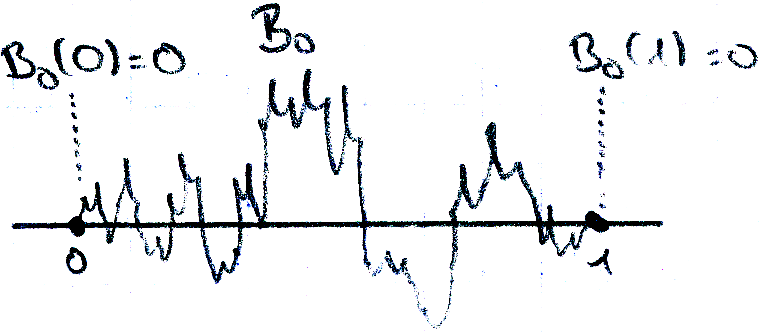
\includegraphics[width=1\textwidth]{./pics/MSTAT002.png}
		\caption{Brownsche Brücke}
		\label{AbbBrownscheBruecke}
	\end{center}
\end{figure}
%Ferger: „Brücke ist doch so'n Ding, da geht man rüber über den Fluss.“
%Ferger: "Also über die Brücke würde ich jetzt nicht gehen. Kein Ahnung, warum man Brücke dazu sagt." → dieses Jahr hat er eine "super" Deutung: ein Charakteristikum einer Brücke
% ist, dass man bei Niveau losgeht und wieder bei Niveau 0 ankommt.

%T_n^\ast ist Supremumsnorm von Partialsummenprozess?+

Es gilt (vergleiche \cite[Seite 34]{shorack2009empirical}%Shorak und Wellner 1986 \undefine{empirical processes}, Seite 34)
\begin{align*}
	H_0(x) &:= \P \argu{\sup_{0 ≤ t ≤ 1} \abs{B_0(t)} ≤ x}
	\overset{\text{Doob}}{=}
	% Doob war ein Mathematiker, der das ausgerechnet hat
	1 - \sum_{k≥ 1}(-1)^{k+1} \exp\argu{-2 k^2 x^2} & ∀ x > 0 \\
	H_0(x) &~= 0 & ∀ x ≤ 0
\end{align*}
$H_0$ ist stetig auf $ℝ$ und streng monoton auf $\intervallHO0{∞}$.
Folglich ist der Test
% für uns: Details wie oben ergänzen
\begin{align*}
	H_0\text{ verwerfen }:⇔ T_n^\ast>H_0^{-1}(1-α)
\end{align*}
ein asymptotischer Niveau-$α$-Test, d.\,h.
\begin{equation*}
	\P_{H_0}(\text{$H_0$ wird verworfen}) = \P_{H_0}(T_n^* > H_0^{-1}(1-α)) \ntoinf α
\end{equation*}
Die Quantilfunktion $H_0^{-1}$ ist in Computerprogrammpaketen implementiert,
z.\,B.\ in MATHEMATICA.
$H_0$ ist die Verteilungsfunktion der \define{Kolmogorov-Smirnov-Verteilung}.

Falls $μ,σ^2$ unbekannt, aber $ν>μ$, so betrachte
\begin{align*}
	\tilde{T}_n&:=\frac1{√n \hat{σ}_n} \max_{0 ≤ k ≤ n} \klammern{\sum_{i=1}^k X_i - \overline{X}_n}
\end{align*}
Vollkommen analog folgt: $\tilde{T}_n\distrto \sup_{0≤ t≤ 1} B_0(t)$ unter $H_0$.
% Beträge in T_n^* kommt von Unwissen, was von ν und μ größer ist, wenn man das weiß, dass ν > μ, so fallen nur die Beträge weg
% folgende Zeilen wurden WiSe 2019/20 dann weggelassen aus Zeitgründen: (bis "Anstelle")
Es gilt (vergleiche z.\,B.\ \cite[Seite 322]{gaensslerstute1977Wahrscheinlichkeitstheorie}%Gänssler + Stute (1977) \undefine{Wahrscheinlichkeitstheorie}, Seite 322)
\begin{align*}
	H_0^+(x) &:= \P\argu{\sup_{0≤ t≤ 1} B_0(t) ≤ x} = 1 - \exp\argu{-2 x^2} & ∀ x ≥ 0 \\
	H_0^+(x) &:= 0 & ∀ x < 0
\end{align*}
Da
\begin{align*}
	(H_0^+)^{-1}(1-α)&=\klammern{-\frac{1}{2}·\log(α)}^{\frac{1}{2}}
\end{align*}
folgt, dass der (einseitige) Test
\begin{align*}
	H_0\text{ verwerfen}:⇔\tilde{T}_n>\klammern{-\frac{1}{2}·\log(α)}^{\frac{1}{2}}
\end{align*}
ein asymptotischer Niveau-$α$-Test für $H_0$ ist.

Anstelle von
\begin{align*}
	T_n^\ast = \frac1{√n \hat{σ}_n} \max_{0≤ k ≤ n}
	\abs[\bigg]{\underbrace{\sum_{i=1}^k \klammern[\big]{X_i - \overline{X}_n}}_{=: C_k}}
\end{align*}
(die $C_k$ heißen \define{kumulierte Summe}) betrachtet \cite{csorgo1997limit} %Csörgő und Horváth (1977) in \undefine{Limit Theorems in Change-point Analysis}
\emph{gewichtete} kumulierte Summen:
\begin{align*}
	U_n^\ast &:= √{n} \frac{1}{\hat{σ}_n} \max_{1≤ k≤ n-1} \frac{\abs{C_k}}{√{k (n - k)}}
\end{align*}

\begin{thm}[Csörgő und Horváth]\label{theoremCH} %noNumber
	Seien
	\begin{align*}
		A_n &:= √{2 \log\argu[\big]{\log(n)}}\\
		D_n &:= 2 \log\argu[\big]{\log(n)} + \frac12 \log\argu[\Big]{\log\argu[\big]{\log(n)}} - \frac12 \log(π) % \qquad ∀ n ≥ n_0 % keine Ahnung, was das soll
	\end{align*}
	Dann gilt unter $H_0$:
	\begin{align}\label{eqTheoremCsorgoHorvath}\tag{1}
		\limn \P_{H_0} \argu[\Big]{A_n U_n^\ast - D_n ≤ t} = \exp\argu[\big]{-2 \exp(-t)} = e^{-2 e^{-t}} =: G(t)
		\qquad ∀ t ∈ ℝ
	\end{align}
	$G$ ist die sogenannte \define{Gumbel-Verteilung}.
\end{thm}

Damit ist die Konstruktion eines asymptotischen Niveau-$α$-Tests für $H_0$ wie folgt möglich: Sei
\begin{align*}
	t_α &:= G^{-1}(1-α) = -\log\argu{-\frac12 \log(1-α)}
\end{align*}
Klarerweise gilt:
\begin{align*}
	A_n U_n^\ast - D_n > t_α ⇔ U_n^\ast > \frac{t_α + D_n}{A_n} := d_n(α)
\end{align*}
Somit ist
\begin{align*}
	H_0\text{ verwerfen}:⇔ U_n^\ast>d_n(α)
\end{align*}
ein asymptotischer Niveau-$α$-Test, d.\,h.
\begin{align}\label{eqUnderTheoremCsorgoHarcath}\tag{2}
	\limn\P_{H_0}\klammern[\big]{U_n^\ast>d_n(α)}
	= \limn \P_{H_0} \argu[\big]{A_n U_n^* - D_n > t_{α}}
	\overset{\eqref{eqTheoremCsorgoHorvath}}{=} 1 - G(t_{α}) = α
\end{align}
\define{Problem:} Die Konvergenz in \eqref{eqTheoremCsorgoHorvath} und damit in \eqref{eqUnderTheoremCsorgoHarcath} ist sehr sehr sehr laaaaaangsaaaam. %genauso stand das an der Tafel
% im 2. Jahr nur das zweite a vervielfacht
% CHECKED: 'bzw.' used.
%Ferger: "[...] Grottenschlecht."
% „n geht gegen ∞, aber das Leben ist endlich“
Andererseits führen die Gewichte in $\klammern[\big]{k (n - k)}^{ -\frac{1}{2} }$ in $U_n^\ast$ zu einer verbesserten Sensitivität (Güte) des \define{$U_n^\ast$-Tests} unter der Alternative ($H_1$), \emph{insbesondere}, falls $τ_n$ nahe bei $1$ oder $n-1$ (\enquote{am Rand}) liegt.
\paragraph{Idee:}% Bei der Bratwurscht. Prof. Ferger hatte diese Idee während eine Bratwurscht in der Pfanne brutzelte.
Weiterhin gewichten, aber durch die einzelne (das heißt von $k$ unabhängige)
und \emph{zufällige} Größe $√{\hat{k}_n (n-\hat{k}_n)}$ wobei
\begin{align*}
	\hat{k}_n &:= \min \set{ 1 ≤ k ≤ n : \abs{C_k} = \max_{1 ≤ j ≤ n-1} \abs{C_j} } \\
						% &= \text{kleinste Maximalstelle des Prozesses $j ↦ C_j$} \\
	C_j &:= \sum_{i=1}^j \klammern[\big]{X_i-\overline{X}_n}
\end{align*}
d.\,h.\ $\hat{k}_n$ ist die kleinste Maximalstelle von $\abs{C_k},k∈\set{1,…,n-1}$. Erhalte:
\begin{align*}
	R_n = \frac{√n}{\hat{σ}_n}
	\frac{\max_{1 ≤ k ≤ n-1} \abs{ \sum_{i=1}^k (X_i-\overline{X}_n) }}{√{\hat{k}_n (n - \hat{k}_n)}}
\end{align*}

\begin{thm}[Dietmar Ferger, 2018, \cite{ferger2018supremum}]%\liabel{theoremFerger2018} %nonumber
	Sei $X_{1n}, ..., X_{nn}$ ein Dreiecksschema von \iid\ Zufallsvariablen mit positiver endlicher Varianz. Dann gilt:
	\begin{align}\label{eqTheoremFerger2018}\tag{3}
		R_n &\distrto R
		\qquad \text{wobei} \qquad
		R = \frac{M}{√{T (1 - T)}} \mit \\
		M &:= \sup_{0 ≤ t ≤ 1} \abs{B_0(t)} \nonumber,\qquad
		T:=\argmax_{0<t<1} \abs{B_0(t)}, \qquad
		B_0=\text{ Brownsche Brücke}\nonumber
	\end{align}
\end{thm}

In diesem Theorem %\ref{theoremFerger2018}
werden Dichte und Verteilungsfunktion $F_R$ von $R$ explizit bestimmt
($F_R$ hat Reihendarstellung).
%Ferger: "Sie müssen immer eine Anwendung haben. Am besten Sie retten die Welt."
Falls $r_α:=F_R^{-1}(1-α)$, so liefert \eqref{eqTheoremFerger2018} für den Test
\begin{align*}
	H_0\text{ verwerfen}:⇔ R_n>r_α
\end{align*}
dass gilt:
\begin{align*}
	\limn\P_{H_0}\klammern[\big]{R_n>r_α}=α
\end{align*}

\begin{bemerkung}
	\eqref{eqTheoremFerger2018} gilt für $X_{1,n},…,X_{n,n}$ \iid\ $∀ n∈ℕ$.\\
	In Monte-Carlo-Simulationen zeigt der $R_n$-Test eine deutlich bessere Güte als der $U_n^\ast$-Test von Csörgő und Horvath.

	Falls bekannt ist, dass $ν>μ$, so betrachte
	\begin{align*}
		R_n^+&:=√{n}·\frac{1}{\hat{σ}_n}·\frac{\max_{1≤ k≤ n-1}\sum_{i=1}^k\klammern[\big]{X_i-\overline{X}_n}}{√{\hat{k}_n^+·\klammern[\big]{n-\hat{k}_n^+}}}\\
		\hat{k}_n^+&:=\min\set{ 1≤ k≤ n-1:C_k=\max_{1≤ j≤ n-1}C_j}
	\end{align*}
\end{bemerkung}
\footnote{Folgendes wurde im Wintersemester 2019/2020 erwähnt:

	Es gilt:
	\begin{align*}
		R_n^+\distrto  R^+=\frac{M^+}{√{T^+·(1-T^+)}},\qquad
		M^+=\sup B_0(t),\qquad
		T^*=\argmax B_0(t)\\
		H^+(x) := \P\argu[\big]{R^+≤ x}
		= 2 Φ(x) - √{\frac2{π}} x \exp\argu{-\frac12 x^2} - 1
		\qquad x ≥ 0 ~ (=0, x<0)
	\end{align*}
	Hierbei ist $Φ$ die Verteilungsfunktion der Standardnormalverteilung. Ferner gilt:
	Die Zufallsgrößen $R^+$ und $T^+$ sind stochastisch unabhängig!
	\begin{align*}
		\hat{τ}_n-τ_n\distrto V &= \\
		% todo: something is missing!
		\hat{τ}_n &:= \argmax_{1≤ k≤ n-1} \abs{\sum_{i=1}^k\klammern[\big]{X_i - \overline{X_n}}}
	\end{align*}
}


	% !TEX root = MSTAT19.tex
% This work is licensed under the Creative Commons
% Attribution-NonCommercial-ShareAlike 4.0 International License. To view a copy
% of this license, visit http://creativecommons.org/licenses/by-nc-sa/4.0/ or
% send a letter to Creative Commons, PO Box 1866, Mountain View, CA 94042, USA.

\subsection{Verteilungskonvergenz in \texorpdfstring{$C(ℝ)$}{C(R)}}
Häufig hat man mit stochastischen Prozessen zu tun, deren Pfade in
\begin{align*}
	C(ℝ):=\set[\Big]{ f:ℝ⟶ℝ:f\text{ stetig}}
\end{align*}
liegen (siehe Beispiel \ref{lemmaMedian} Median ganz am Anfang). Die bisherige Theorie für $C(I)$ mit
\emph{kompaktem} Intervall $I$ deckt das nicht ab. Wir versehen $C(ℝ)$ mit der Metrik
\begin{align*}
	d(f,g) &:= \sum_{j≥ 1} 2^{-j} \frac{d_j(f,g)}{1+d_j(f,g)} & ∀ f, g ∈ C(ℝ)\\
	d_j(f,g) &:= \sup_{-j ≤ t ≤ j} \abs{f(t)-g(t)} & ∀ f, g ∈ C(ℝ)
\end{align*}
Aus der Analysis ist bekannt, dass $\klammern[\big]{C(ℝ),d}$ ein vollständiger separabler metrischer Raum ist. Ferner gilt:
\begin{align*}
	d(f_n,f)\ntoinf 0
	⇔ ∀ j∈ℕ: d_j(f_n,f)\ntoinf 0
	⇔\text{glm. Konvergenz auf Kompakta}
\end{align*}
Deshalb heißt $d$ die Metrik der gleichmäßigen Konvergenz auf Kompakta.

Seien $π_t \colon C(ℝ) ⟶ ℝ$ und $π_T \colon C(ℝ) ⟶ ℝ^{\measure{T}}$ die Projektionsabbildungen, d.\,h.\ z.\,B.
\begin{align*}
	π_T(f)=\klammern[\big]{f(t)}_{t∈ T}=\klammern[\big]{f(t_1),…,f(t_k)}\qquad
	T=\set{ t_1,…, t_k}
\end{align*}

\begin{theorem}\label{theorem7.20}
	\begin{align*}
		\B_d\klammern[\big]{C(ℝ)} &= σ \argu[\big]{π_t : t ∈ ℝ} = σ \argu[\big]{π_T : T ⊆ ℝ\text{ endlich}}
	\end{align*}
\end{theorem}

\begin{proof}
	Die Argumente im Beweis von Satz \ref{satz7.2} lassen sich problemlos übertragen,
	da $C(ℝ)$ ebenfalls separabel ist.
\end{proof}

Ebenfalls analog (zu \ref{satz7.3}) beweist man:

\begin{satz}\label{satz7.21}
	 Sei $(Ω,\A)$ messbarer Raum und $C:=C(ℝ)$ versehen mit $\B_d(C)$.
	 Dann gilt für eine Abbildung $X \colon Ω⟶ C(ℝ)$:
	 \begin{align*}
	 	X~\A\text{-}\B_d(C)\text{-messbar}
	 	⇔∀ t∈ℝ:
	 	π_t∘ X~\A\text{-}\B(ℝ)\text{-messbar }
	 \end{align*}
\end{satz}

Konsequenz aus Satz \ref{satz7.21}: Jeder stetige stochastische Prozess indiziert nach $ℝ$ kann aufgefasst werden als Zufallsvariable in $\klammern[\big]{C(ℝ),d}$.

\begin{satz}\label{satz7.22}
	Seien $X,Y$ Zufallsvariablen in $\klammern[\big]{C(ℝ),d}$. Dann gilt:
	\begin{align*}
		X\stackeq{\L}Y⇔
		\klammern[\Big]{X(t_1),…,X(t_k)}\stackeq{\L}\klammern[\Big]{Y(t_1),…,Y(t_k)}
	\end{align*}
	für jede Wahl von Punkten $t_1<…<t_k$ aus $ℝ$.
\end{satz}

\begin{proof}
	Siehe Theorem \ref{theorem7.20} + Maßeindeutigkeitssatz.
\end{proof}

Der folgende Satz zeigt, dass sich der Nachweis der Verteilungskonvergenz in $\klammern[\big]{C(ℝ), d}$ zurückführen lässt auf den in $\klammern[\Big]{C \argu[\big]{\intervall{-j}{j}}, d_j} ~ ∀j ∈ ℕ$.

Für $f∈ C(ℝ)$ sei
\begin{align*}
	I_j &:= \intervall{-j}j, & f^{(j)} &:= \restr{f}{I_j},\\
	\text{ d.\,h.\ } f^{(j)} &\colon I_j ⟶ ℝ, & f^{(j)}(t) &:= f(t) & ∀ t ∈ I_j
\end{align*}

\begin{satz}[Ward Whitt, 1970] \label{satz7.23}
	Seien $X,X_n,n∈ℕ$ Zufallsvariablen in $\klammern[\big]{C(ℝ),d}$. Dann gilt:
	\begin{align*}
		X_n\distrto X\text{ in }\klammern[\big]{C(ℝ),d}
		⇔∀ j∈ℕ:
		X_n^{(j)}\distrto  X^{(j)}\text{ in }\klammern[\big]{C(I_j),d_j}
	\end{align*}
\end{satz}

Satz \ref{satz7.23} geht auf \cite{whitt1970weak} zurück. Ein (relativ) einfacher Beweis findet sich in \cite[Seite 260]{kallenberg2006foundations}.% Kallenberg (1997), \undefine{Foundations of modern probability}, Seite 260.

\begin{bemerkungnr}\label{bemerkung7.24}\
	\begin{enumerate}[label=(\alph*)]
		\item \label{it:7.240inf} Die Resultate in \ref{theorem7.20},\ref{satz7.21},\ref{satz7.22} und \ref{satz7.23} gelten analog für $C\klammern[\big]{\intervallHO0{∞}}$ mit $I_j$ ersetzt durch $[0,j]$.
		\item \label{it:7.24runterbrechen} Satz \ref{satz7.23} ermöglicht es insbesondere, auf die Konvergenzkriterien in \ref{satz7.9} und \ref{satz7.11MomentenkriteriumVonKolmogoroff} zurückzugreifen.
	\end{enumerate}
\end{bemerkungnr}

\begin{beispiel}\label{beispiel7.25}
	Seien $(ξ_i)_{i∈ℕ}$ \iid\ mit $\Earg{ξ_1}=0$, $\Var(ξ_1)=1$ und
	\begin{align*}
		S_k&:=\sum_{j=1}^kξ_j\qquad∀ k∈ℕ_0\\
		X_n(t) &:= \frac1{√n} S_{\floor{n t}}
		+ \frac1{√n} \klammern[\big]{n t - \floor{n t}} ξ_{\floor{n t} + 1}
		\qquad ∀ t ∈ \intervallHO0{∞}
	\end{align*}
	D.\,h. $X_n$ ist Polygonzug durch $\klammern{ \frac kn, \frac1{√n} S_n }, k ∈ ℕ_0$.
	Aus Satz \ref{satz7.16Donsker} folgt:
	\begin{align*}
		X_n^{(j)}\distrto B^{(j)} \quad ∀ j ∈ ℕ \quad
		&\overset{\ref{bemerkung7.24}\ref{it:7.240inf} )+ \ref{satz7.23}}{⇔}
		X_n\distrto  B \text{ in } \klammern[\Big]{C\argu[\big]{\intervallHO0{∞}},d}
	\end{align*}
\end{beispiel}

	% !TEX root = MSTAT19.tex
% This work is licensed under the Creative Commons
% Attribution-NonCommercial-ShareAlike 4.0 International License. To view a copy
% of this license, visit http://creativecommons.org/licenses/by-nc-sa/4.0/ or
% send a letter to Creative Commons, PO Box 1866, Mountain View, CA 94042, USA.

\section{Argmin-Theoreme in \texorpdfstring{$C(ℝ)$}{C(R)}} %8
Erinnere an folgende Probleme, vergleiche Gleichungen \eqref{eq1.2} und \eqref{eq1.5} in Kapitel \ref{sec:median} zum Median.
Wann überträgt sich die Konvergenz (f.\,s.\ oder in Verteilung) von stetigen stochastischen Prozessen auf deren Minimalstellen?

\begin{definition}\label{definition8.1}
	Sei $f∈ C(ℝ)$.
	\begin{enumerate}[label=(\arabic*)]
		\item $\begin{aligned}
			A(f):=\argmin(f):=\set{ t∈ℝ:f(t)=\inf_{s∈ℝ} f(s)}
			\end{aligned}$ = Menge aller Minimalstellen
		\item $τ∈ A(f)$ heißt \define{wohl-separiert}
			\begin{align*}
				:⇔\inf\set[\Big]{ f(t):\abs{t-τ}≥ε}>f(τ)\qquad∀ 0<ε∈ℚ
			\end{align*}
	\end{enumerate}
\end{definition}

\begin{bemerkungnr}\label{bemerkung8.2}\
	\begin{enumerate}[label=(\arabic*)]
		\item $A(f)\neq∅$ ist natürlich nicht ausgeschlossen, aber in jedem Fall ist $A(f)$ \emph{abgeschlossen} in $ℝ$, denn:
		Sei $(t_n)_{n ∈ ℕ}$ eine Folge in $A(f)$ mit $t_n \ntoinf t$. Dann gilt:
		\begin{align*}
			f(t)&=\limn\underbrace{f(t_n)}_{=\inf_{s∈ℝ}f(s)}=\inf_{s∈ℝ}f(s)
			⇒ t∈ A(f)
		\end{align*}
		\item $τ$ wohl-separiert $⇒τ$ eindeutig, denn:
		Sei $\tilde{τ}∈ A(f)$ und $\tilde{τ}\neqτ$. Also:
		\begin{align}\label{eqBemerkung8.2Stern}\tag{$\ast$}
			∃ 0 &< ε ∈ ℚ :
			\abs[\big]{τ - τ} > ε \\
			\nonumber
			\inf_{s∈ℝ}f(s)
			\overset{\tilde{τ}∈ A(f)}&=
			f(τ)
			\overset{\eqref{eqBemerkung8.2Stern}}{≥}
			\inf\set[\Big]{ f(t):\abs{t-τ}≥ε}
			\overset{τ\text{ wohl-sep}}{>}
			f(τ)
			\overset{τ∈ A(f)}{=}
			\inf_{s∈ℝ} f(s)
		\end{align}
		Dies ist ein Widerspruch!
		\item Wohl-separiertheit ist also eine stärkere Bedingung als Eindeutigkeit der Minimalstelle.
			Sie schließt \enquote{degenerierte} Fälle wie in Abbildung \ref{AbbMinimalstelleEindeutigNichtWohlsepariert} aus.
	\end{enumerate}
\end{bemerkungnr}

\begin{beisp}
	Wann ist eine Minimalstelle eindeutig, aber nicht wohlsepariert?
	\begin{figure}[H]
		\begin{center}
			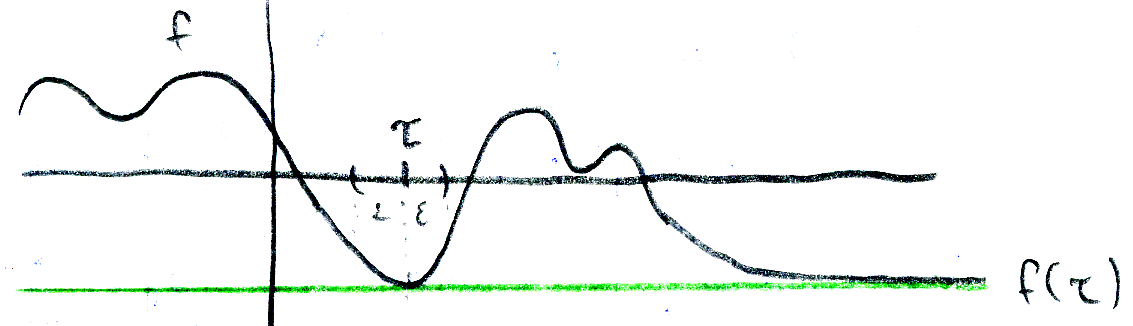
\includegraphics[width=1\textwidth]{./pics/MSTAT003.png}
			\caption{$τ$ eindeutig, aber das Infimum von $f$ außerhalb von $\intervallO{τ-ε}{τ+ε}$ ist auch $f(τ)$!}
			\label{AbbMinimalstelleEindeutigNichtWohlsepariert}
		\end{center}
	\end{figure}
\end{beisp}

\begin{satz}\label{satz8.3}
	Seien $f,f_n$, $n∈ℕ$ aus $C(ℝ)$, $τ_n∈ A(f_n)\neq∅~∀ n≥ N_0∈ℕ$
	(also $τ_n$ ist eine Minimalstelle, ab einem gewissen Zeitpunkt $N_0$.)
	und $τ∈ A(f)$ sei wohl-separiert.
	Falls
	\begin{align}\label{eqSatz8.3_1}\tag{1}
		\norm[\big]{ f_n-f}\overset{\text{Def}}{=}\sup_{t∈ℝ}\abs[\big]{f_n(t)-f(t)}\ntoinf 0
	\end{align}
	so folgt
	\begin{align*}
		τ_n\ntoinf τ
	\end{align*}
\end{satz}

\begin{proof}
	Sei o.\,B.\,d.\,A.\ $0 < ε ∈ ℚ$. Es folgt:
	\begin{align*}
		s(ε)&:=\inf\set[\big]{ f(t):\abs{t-τ}≥ε}
		\overset{\text{Def wohl-sep}}{>}
		f(τ)\\
		⇒
		δ &:= δ(ε) := \frac13 \klammern[\big]{s(ε) - f(τ)} > 0 \\
		\overset{\eqref{eqSatz8.3_1}}{⇒}
		∃ n_0&=n_0(δ)∈ℕ:∀ n≥ n_0:
		\norm{ f_n-f}≤δ
	\end{align*}
	Für alle $n≥\max(N_0,n_0)$ gilt:

	Falls $t∈ℝ$ mit $\abs{t-τ}≥ε$, so folgt:
	\begin{align*}
		f_n(t)-f_n(τ)
		&=\underbrace{f_n(t)-f(t)}_{≥\underbrace{-\underbrace{\norm{ f_n-f}}_{≤δ}}_{≥-δ}}+\underbrace{\underbrace{f(t)}_{≥ s(ε)}-f(τ)}_{≥ s(ε)-f(τ)=3δ}+\underbrace{f(τ)-f_n(τ)}_{≥-δ}\\
		&≥ -δ + 3δ - δ %\\
		%&
		= δ > 0
	\end{align*}
	Es folgt
	\begin{align}\label{eqProofSatz8.3Stern}\tag{$\ast$}
		f_n(t)>f_n(τ)\qquad∀ t∈ℝ\mit\abs{t-τ}≥ε
	\end{align}
	Folglich gilt $\abs{τ_n-τ}<ε$, denn sonst folgte aus \eqref{eqProofSatz8.3Stern}, dass
	$f_n(τ_n)>f_n(τ)$ im Widerspruch zu $τ_n$ ist Minimalstelle von $f_n$.

	Somit ist gezeigt:
	\begin{align*}
		∀ ε ∈ ℚ ∩ \intervallO0{∞} : ∃ m_0 = m_0(ε) := \max(N_0, n_0) : ∀ n ≥ m_0 : \abs{τ_n-τ} < ε
		& \qedhere
	\end{align*}
\end{proof}

Satz \ref{satz8.3} lässt sich problemlos von $ℝ$ auf offene Intervalle $I = \intervallO ab$ übertragen.

Für kompakte Intervalle $I=\intervall ab$, $a < b ∈ ℝ$ muss $τ$ nur eindeutig sein.
Es gilt:

\begin{satz}\label{satz8.4}
	Sei $I=\intervall ab$ kompaktes Intervall und seien $f,f_n$, $n∈ℕ$ aus $C(I)$.
	Dann gilt:
	\begin{enumerate}[label=(\arabic*)]
		\item \label{it:8.4argminexistenz} $\begin{aligned}
			A(f_n)\neq∅\qquad∀ n∈ℕ
		\end{aligned}$
		\item \label{it:8.4argminkonv} Falls $τ$ \emph{eindeutige} Minimalstelle von $f$ ist und falls
			\begin{align*}
				\norm{ f_n-f}_I:=\sup_{t∈ I}\abs[\big]{f_n(t)-f(t)}\ntoinf 0
			\end{align*}
			so gilt für \emph{jede} Auswahl $τ_n ∈ A(f_n)$:
			$τ_n\ntoinf τ$
	\end{enumerate}
\end{satz}

%Ferger: "In irgendeinem der Seminarräumen ist mal eine Tafel von der Wand gefallen. Und ich möchte jetzt nicht unter so einer Tafel begraben liegen.
% Vielleicht ist das für einen Professor ein schöner Tod. Aber bitte jetzt noch nicht."
% "Ich bin ja von Natur aus etwas ängstlich. Es gab da mal so ein lustiges Lied und da singt der Sänger: "Leute seid nicht feige, lasst mich ...""

\begin{proof}
	\ref{it:8.4argminexistenz} gilt, da jede stetige Funktion auf einem Kompaktum das Infimum annimmt.
	\paragraph{Zeige \ref{it:8.4argminkonv}:}
	$τ$ ist wohl-separiert auf $I$, denn:
	Angenommen, es wäre nicht so, also angenommen
	\begin{align*}
		∃0<ε∈ℚ:\inf\set[\big]{ f(t):t∈ I:\abs{t-τ}≥ε}=f(τ)
	\end{align*}
	Die Menge $K_ε:=\set{ t∈ I:\abs{t-τ}≥ε}$ ist kompakt.
	Weil $f$ stetig ist, nimmt $f$ auf $K_ε$ ihr Infimum an, d.\,h.
	\begin{align*}
		∃σ∈ I:\abs{σ-τ}≥ε\mit f(σ)=\inf
		\set[\big]{ f(t):t∈ I:\abs{t-τ}≥ε}
		=f(τ)
	\end{align*}
	Also ist $σ$ eine \emph{weitere} Minimalstelle von $f$ (denn $σ$ und $τ$ haben positiven Abstand zueinander) im Widerspruch zur Eindeutigkeit von $τ$.

	Jetzt weiter wie im Beweis von Satz \ref{satz8.3}.
\end{proof}

Es ergeben sich nun mühelos Argmin-Theoreme für fast sichere Konvergenz:

\begin{satz}\label{satz8.5}
	Seien $M=\set[\big]{ M(t):t∈ ℝ}$, $M_n=\set[\big]{ M_n(t):t∈ ℝ}$, $n∈ℕ$ stochastische Prozesse
	über $(Ω,\A,\P)$ mit Pfaden in $C(ℝ)$ (d.\,h.\ $M\colon ℝ⟶ℝ,~t↦ M(t,ω)$ stetig für alle $ω∈Ω$).
	Es gelte:
	\begin{enumerate}[label=(\arabic*)]
		\item \label{it:8.5tauIsMin} Es gilt
			\begin{align*}
				τ(ω)∈ A\klammern[\big]{M(·,ω)}\overset{\Def}{=}
				\argmin\klammern[\big]{M(·,ω)}
				\overset{\Def}{=} \set[\Big]{t ∈ R : \inf_{s ∈ ℝ} M(s, ω) = M(t, ω)}
				\text{f.\,s.}
			\end{align*}
			für eine Zufallsvariable $τ \colon Ω ⟶ ℝ$,
			also $\P\argu[\big]{\set[\big]{ω ∈ Ω : τ(ω) ∈ A\argu{M(·, ω)}}} = 1$
		\item \label{it:8.5wohlsep} $\begin{aligned}
			\inf \set[\big]{ M(t) : \abs{t - τ} ≥ ε} > M(τ) \text{ f.\,s. }\qquad ∀\, 0 < ε ∈ ℚ
		\end{aligned}$ (wohl-separiertheit)
		\item \label{it:8.5Konvergenz} $\begin{aligned}
			\norm[\big]{M_n-M}_∞\ntoinf 0\text{ f.\,s.}
		\end{aligned}$
	\end{enumerate}
	Dann gilt für jede Folge $(τ_n)_{n∈ℕ}$ von Zufallsvariablen mit $τ_n∈ A(M_n)$ f.\,s.:
	$τ_n\ntoinf τ$ f.\,s.
\end{satz}

\begin{proof}
	Setze
	\begin{align*}
		Ω_0 := \underbrace{
			\set[\Big]{ω ∈ Ω : τ(ω) ∈ A \argu[\big]{M(·, ω)}}
		}_{=: \set[\big]{τ ∈ A(M)} \text{ Einsmenge wg \ref{it:8.5tauIsMin}}}
		& ∩ \bigcap_{0 < ε ∈ ℚ}
		\overbrace{
			\underbrace{
				\set[\Big]{ \inf \set[\big]{ M(t) : \abs{t - τ} ≥ ε} > M(τ)}
			}_{\text{Einsmenge wg.\ \ref{it:8.5wohlsep}}}
		}^{ \hat{=} \text{wohl-separiert}}\\
		& ∩
		\underbrace{
			\set[\Big]{ \norm{ M_n - M} \ntoinf 0}
		}_{\text{Einsmenge wg \ref{it:8.5Konvergenz}}}
		∩ \bigcap_{n ≥ 1}
		\underbrace{
			\set[\Big]{τ_n ∈ A(M_n)}
		}_{\text{Einsmenge nach Vor.}}
	\end{align*}
	Erinnerung: Abzählbare Schnitte von Einsmengen sind Einsmengen.
	Dann gilt $\P(Ω_0)=1$.

	Satz \ref{satz8.3} besagt, dass für alle $ω ∈ Ω_0$ die Konvergenz
	der Mininmalstellen $τ_n(ω) → τ(ω)$ gilt. Also gilt $τ_n → τ$ fast sicher.
	% Da $Ω_0\overset{\ref{satz8.3}}{⊆}\set[\big]{τ_n\ntoinf τ}$, folgt die Behauptung.
\end{proof}

Analog erhält man mit Satz \ref{satz8.4}:

\begin{satz}\label{satz8.6}
	Seien $M,M_n,n∈ℕ$ stochastische Prozesse über $(Ω,\A,\P)$ mit Pfaden in $C(I)$,
	wobei $I$ kompaktes Intervall ist.
	Es gelte:
	\begin{enumerate}[label=(\arabic*)]
		\item \label{it:8.6eindeutig} Es gibt eine Zufallsvariable $τ$, die f.\,s.\ eindeutige Minimalstelle von $M$ ist.
		\item \label{it:8.6fskonvergenz} $\begin{aligned}
			\norm{ M_n-M}_I\ntoinf 0
		\end{aligned}$ f.\,s.
	\end{enumerate}
	Dann gilt für jede Folge $(τ_n)_{n∈ℕ}$ von Zufallsvariablen mit $τ_n∈ A(M_n)$ f.\,s.:
	$τ_n\ntoinf τ$ f.\,s.
\end{satz}

\begin{proof}
	Setze
	\begin{align*}
		 Ω_0&:=\set{τ\text{ ist eindeutige Minimalst. v. }M}
		 ∩\set[\Big]{\norm{ M_n-M}_I\ntoinf 0}
		 ∩\bigcap_{n≥1}\set[\Big]{τ_n∈ A(M_n)}\\
		 &⇒\P(Ω_0)=1
	\end{align*}
	Da $Ω_0\overset{\ref{satz8.4}}{⊆}\set[\Big]{τ_n\ntoinf τ}$, folgt die Behauptung.
\end{proof}



	% !TEX root = MSTAT19.tex
% This work is licensed under the Creative Commons
% Attribution-NonCommercial-ShareAlike 4.0 International License. To view a copy
% of this license, visit http://creativecommons.org/licenses/by-nc-sa/4.0/ or
% send a letter to Creative Commons, PO Box 1866, Mountain View, CA 94042, USA.

\subsection{Anwendung in der Change-Point-Analyse} \label{sec:AnwendungCPA} %8.2 % neu: 8.1
Betrachten des Change-Point-Modell aus Kapitel \ref{sec:donskeranwendung}:
$X_{1, n}, …, X_{n, n}$, $n∈ℕ$ seien unabhängige reelle Zufallsvariablen mit
\begin{align*}
	\begin{cases}
		X_{i,n} \:\iid \sim(μ,σ^2), & \falls 1 ≤ i ≤ τ_n\\
		X_{i,n} \:\iid \sim(ν,τ^2), & \falls τ_n < i ≤ τ_n
	\end{cases}
	, \qquad μ \neq ν
\end{align*}
Mit $τ_n∈\set[\big]{1,…,n-1}$ unbekannter \define{Wechselzeitpunkt}.
\begin{align*}
	\underbrace{X_1,…,X_{τ_n}}_{\text{pre-change variables}},\underbrace{X_{τ_n+1},…,X_n}_{\text{post-change variables}}
\end{align*}

\paragraph{Ziel:} Schätzung von $τ$.

Schreibe im Folgenden: $X_i\equiv X_{i,n}$
\begin{align*}
	S_k &:= \sum_{i=1}^k \klammern[\big]{X_i-\overline{X}_n}  &∀& \, 0 ≤ k ≤ n \\
	\overline{X}_n &:= \frac{1}{n} \sum_{i=1}^n X_i &∀& n ∈ ℕ \\
	θ_n&:=\frac{τ_n}{n} &∀& n∈ℕ
\end{align*}

Eine elementare Rechnung zeigt (zur Übung, ist wirklich  einfach):
\begin{align}\label{eqUnder8.2_1}\tag{1}
	\Earg{S_k}
	&=
	\begin{cases}
		k·(1-θ_n)·(μ-ν), &\falls 0≤ k≤τ_n \quad \text{(monoton wachsend)}\\
		% kμ - k(1/n (τ μ + (n-τ) ν)) = k (μ - θμ - (1 - θ)ν) = k (1 - Θ)(μ - ν)
		(n-k)·θ_n·(μ-ν), &\fallsτ_n<k≤ n \quad \text{(monoton fallend)}
		% τμ + (k - τ)ν - k(1/n (τ μ + (n-τ) ν)) = τμ + kν - τν - kθμ - kν + kθν
		% = τμ - τν - kθμ + kθν = (τ - kθ)(μ - ν) = (n - k)θ(μ - ν)
	\end{cases} \\ \nonumber
	\abs[\big]{\Earg{S_k}}
	&=
	\begin{cases}
		k·(1-θ_n)·\abs{μ-ν}, &\falls 0≤ k≤τ_n \quad \text{(monoton wachsend)}\\
		(n-k)·θ_n·\abs{μ-ν}, &\fallsτ_n<k≤ n  \quad \text{(monoton fallend)}
	\end{cases} \\
	&⇒τ_n=\argmax_{0≤ k≤ n}\abs[\big]{\Earg{S_k}}\nonumber
\end{align}

Daraus folgt, dass $\abs[\big]{\Earg{S_k}}$ (in Abhängigkeit von $k$) erst monoton wachsend und ab $k=τ_n$ monoton fallend ist.

\begin{figure}[H] % oder ht!
	\begin{center}
		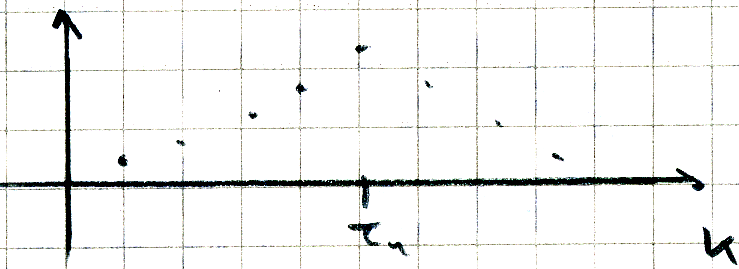
\includegraphics[width=1\textwidth]{./pics/MSTAT004.png}
		\caption{Plot von $\Earg{S_k}$}
		%\label{Abb}
	\end{center}
\end{figure}

Dies motiviert folgenden Schätzer (ersetze unbekannte $\abs[\big]{\Earg{S_k}}$ durch bekannte $\abs{S_k}$):
\begin{align*}
	\hat{τ}_n:=\argmax_{0≤ k≤ n}\abs[\big]{S_k}
\end{align*}
Im Folgenden sei $τ_n=\floor{ n·θ},θ∈(0,1)$.
Wir zeigen:
\begin{align*}
	\hat{θ}_n := \frac{\hat{τ}_n}{n} \ntoinf θ \qquad \P \text{-f.\,s.}
\end{align*}

\define{Annahme:} Wir nehmen die sogenannte \define{Momentenbedingung an}, d.\,h.
\begin{align*}
	μ_p := \Earg[\Big]{ \abs[\big]{X_{τ_n}}^p } < ∞,
	\qquad
	ν_p := \Earg[\Big]{ \abs[\big]{X_{τ_n+1}}^p } < ∞
\end{align*}

Sei $M_n:=$ der Polygonzug durch $\klammern{\frac{k}{n},\frac{1}{n} S_k}$, $0 ≤ k ≤ n$.
Dann folgt aus Lemma \ref{lemma7.17}:
\begin{align*}
	\hat{θ}_n&:=\argmax_{0≤ t≤ 1}\abs[\big]{M_n(t)}\\
	M_n(t) &= \frac{1}{n} S_{\floor{n t}}
	+ \klammern[\big]{n t - \floor{w t}}
	\klammern{ S_{\floor{n t} + 1} - S_{\floor{n t}}} & ∀\, 0 ≤ t ≤ 1 \\
	\Earg{M_n(t)} &=\frac{1}{n} \Earg{ S_{\floor{n t}}} + \klammern{n t - \floor{w t}}
	\klammern{\Earg{S_{\floor{n t} + 1}} - \Earg{S_{\floor{n t}}} } & ∀\, 0 ≤ t ≤ 1 \\
\end{align*}

Sei $\overline{M}_n(t) := \Earg{M_n(t)}$, $0 ≤ t ≤ 1$.
Dann ist $\overline{M}_n$ ein Polygonzug durch die Punkte $\klammern{\frac{k}{n}, \frac{1}{n} \Earg{S_k}}$, $0 ≤ k ≤ n$.
Da wegen \eqref{eqUnder8.2_1}
\begin{align*}
	\overline{M}_n\klammern{\frac{k}{n}}
	&=\frac{1}{n} \Earg[\big]{S_k}
	\overset{\eqref{eqUnder8.2_1}}
	=
	\begin{cases}
		\frac{k}{n} (1-θ_n) (μ-ν) &\falls \frac{k}{n} ≤ \frac{τ_n}{n} = θ_n\\
		\klammern{1-\frac{k}{n}} θ_n (μ-ν), & \falls \frac{k}{n} > θ_n
	\end{cases}
\end{align*}
folgt
\begin{align*}
	\overline{M}_n\klammern{t}
	&=
	\begin{cases}
		t (1 - θ_n) (μ-ν) & \falls t ≤ θ_n \\
		\klammern{1-t} θ_n (μ-ν), & \falls \frac{k}{n} > θ_n
	\end{cases}
\end{align*}
Beachte $θ - \frac{1}{n} < θ_n = \frac{\floor{nθ}}{n} \leq θ$.
Eine Fallunterscheidung ($t≤θ_n$; $θ_n<t≤θ$; $t>θ$) liefert
% θ_n > θ → größte Unterschiede möglich bei θ und θ_n
% alles ·(μ - ν) im Folgenden
% bei θ: θ(1-θ) - θ(1-θ_n) = Θ(θ_n - θ) < θ/n
% bei θ_n: θ_n(1-θ_n) - (1-θ_n)θ = (1-θ_n)(θ_n - θ) < (1-θ_n)/n
% → da könnte auch 1 statt 2 stehen, aber gut, 2 > 1
\begin{align}\label{eqUnder8.2_2}\tag{2}
	\norm[\big]{\overline{M}_n-M}
	&= \sup_{0 ≤ t ≤ 1} \abs[\Big]{\overline{M}_n(t) - M(t)}
	≤ \frac2n \abs{μ-ν} \ntoinf 0 \text{, wobei} \\ \nonumber
	M(t) &=
	\begin{cases}
		t (1-θ) (μ-ν) , & \falls 0 ≤ t ≤ θ\\
		(1-t) θ (μ-ν), & \falls θ < t ≤ 1
	\end{cases}
	\\ \nonumber
	\abs{M(t)} &=
	\begin{cases}
		t (1-θ) \abs{μ-ν} , & \falls 0 ≤ t ≤ θ \\
		(1-t) θ \abs{μ-ν} , & \falls θ < t ≤ 1
	\end{cases}
\end{align}

\begin{figure}[H]
	\begin{center}
		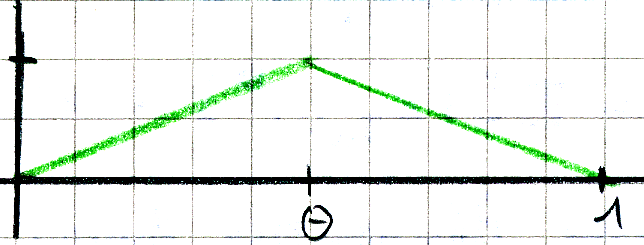
\includegraphics[width=1\textwidth]{./pics/MSTAT005.png}
		\caption{Plot von $M(t)$}
		%\label{AbbTitel}
	\end{center}
\end{figure}

Somit ist dieses $θ$ charakterisierbar als Maximalstelle:
\begin{align*}
	θ=\argmax_{0≤ t≤ 1}\abs[\big]{M(t)}
\end{align*}

Zeige:
\begin{align*}
	\norm[\big]{ M_n-M}
	&= \sup_{0 ≤ t ≤ 1} \abs[\big]{M_n(t)-M(t)} \ntoinf 0 \quad \P\text{-f.\,s.}
\end{align*}
Da
\begin{align}\label{eqUnder8.2_3}\tag{3}
	0≤\norm[\big]{ M_n-M}≤\norm[\big]{ M_n-\overline{M}_n}+\underbrace{\norm[\big]{\overline{M}_n-M}}_{
		\stackrelnew{\eqref{eqUnder8.2_2}}{n⟶∞}{\longrightarrow}0
	}
\end{align}

betrachte den ersten Summanden
\begin{align}\label{eqUnder8.2_4}\tag{4}
	\norm[\big]{M_n - \overline{M}_n}
	= \sup_{0 ≤ t ≤ 1} & \abs[\big]{M_n(t) - \overline{M}_n(t)}
	\overset{\ref{lemma7.17}}{=}
	\max_{0 ≤ k ≤ n} \abs[\bigg]{\underbrace{
			M_n \argu{\frac{k}{n}}
		}_{= \frac{1}{n} S_k}
		- \underbrace{
			\overline{M}_n \argu{\frac{k}{n}}
		}_{=\frac{1}{n} \Earg{S_k}}
	} \\
	\nonumber
	\frac{1}{n} S_k
	&= \frac{1}{n} \sum_{i=1}^k\klammern[\big]{X_i - \overline{X}_n}
	= \frac{1}{n} \sum_{i=1}^k X_i - \frac{k}{n^2} \sum_{i=1}^n X_i \\ \nonumber
	⇒
	M_n \argu{\frac{k}{n}} - \overline{M}_n \argu{\frac{k}{n}}
	\overset{\text{Lin}}&=
	\frac{1}{n} \sum_{i=1}^k \underbrace{
		\klammern[\Big]{X_i - \Earg[\big]{X_i}}
	}_{=:Z_i}
	- \frac{k}{n^2} \sum_{i=1}^n \underbrace{
		\klammern[\Big]{X_i - \Earg[\big]{X_i}}
	}_{=Z_i} \\ \nonumber
	⇒
	\abs{M_n \argu{\frac{k}{n}} - \overline{M}_n \argu{\frac{k}{n}}}
	\overset{\laplace\neq}&{≤}  % laplace is a triangle % Dreiecksungleichung
	\frac{1}{n} \underbrace{
		\abs[\bigg]{\sum_{i=1}^k
			\klammern[\big]{X_i - \Earg[\big]{X_i}}
		}
	}_{
		≤ \max_{0 ≤ k ≤ n} \abs{\sum_{i=1}^k Z_i}
	} + \underbrace{
		\frac{k}{n^2}
	}_{≤\frac{1}{n}}
	\underbrace{
		\abs[\bigg]{\sum_{i=1}^n
			\klammern[\Big]{X_i - \Earg[\big]{X_i}}
		}}_{
			≤\max_{0 ≤ k ≤ n} \abs{\sum_{i=1}^k Z_i}
		} \\ \nonumber
		&≤ \frac{2}{n} \max_{0 ≤ k ≤ n} \abs{\sum_{i=1}^k Z_i}\\
	⇒\label{eqUnder8.2_5}\tag{5}
	& \max_{0 ≤ k ≤ n} \abs{M_n \argu{\frac{k}{n}} - \overline{M}_n \argu{\frac{k}{n}}}
	≤ \frac{2}{n} \max_{0 ≤ k ≤ n} \abs{\sum_{i=1}^k Z_i}
\end{align}

Es ist
\begin{align*}
	T_k=\sum_{i=1}^k Z_i\qquad 0≤ k≤ n
\end{align*}
ein Martingal bzgl.\ der Filtration
\begin{align*}
	\F_k:=σ\klammern[\big]{Z_1,…,Z_k} &\qquad∀ 1≤ k≤ n,\qquad \F_0:=\set{∅,Ω}
\end{align*}
Es ist Martingal, weil
\begin{align*}
	\Earg{T_{k+1}~\middle|~\F_k}
	% CHECKED: '|' used.
	&=\Earg{\klammern{\sum_{i=1}^k Z_i} + Z_{k + 1} ~ \middle| ~ \F_k}
	% CHECKED: '|' used.
	= \underbrace{
		\Earg[\bigg]{ \overbrace{\sum_{i=1}^k Z_i}^{\text{ist $\F_K$-messbar}}
		~\bigg|~ \F_k}
		% CHECKED: '|', '\bigg' used.
	}_{ = T_k}
	% CHECKED: '\bigg' used
	+ \underbrace{\Earg{ Z_{k + 1}~\middle|~\F_k}}_{= \Earg{Z_{k + 1}} = 0}
	% CHECKED: '|' used.
\end{align*}

Es folgt aus der bedingten Jensenungleichung, dass $\klammern{\abs{T_k}^p,\F_k}_{0≤ k≤ n}$ ein nicht-negatives Submartingal ist.
\begin{align}\nonumber
	\P\argu{\norm[\big]{M_n - \overline{M}_n} ≥ ε}
	\overset{\eqref{eqUnder8.2_4}+\eqref{eqUnder8.2_5}}&{≤}
	\P \argu{ \frac{2}{n} \max_{0 ≤ k ≤ n} \abs[\big]{T_k} \geq ε } \\ \nonumber
	&≤ \P\argu{\max_{0 ≤ k ≤ n} \abs[\big]{T_k} ≥ \frac{1}{2} n ε} \\ \nonumber
	\overset{u↦ u^p\uparrow}&{=}
	% tocheck: im original war hier ein \leq statt =, aber es sollte doch = sein, oder?
	% ist auch egal, da eh abgeschätzt wird
	\P \argu{\klammern{\max_{0 ≤ k ≤ n} \abs[\big]{T_k}}^p ≥ \klammern{\frac{1}{2} n ε}^p} \\ \nonumber
	&= \P \argu[\bigg]{\max_{0 ≤ k ≤ n} \underbrace{
		\abs[\big]{T_k}^p
	}_{\text{Submartingal}}
	≥ \underbrace{
		\klammern{\frac{1}{2} nε}^p
	}_{=: y > 0}} \\ \nonumber
	% ⇒
	% \P \argu{\norm[\big]{ M_n - \overline{M}_n} ≥ ε}
	% &≤ \P\argu[\bigg]{\max_{0 ≤ k ≤ n} \underbrace{
		% \abs[\big]{T_k}^p
	% }_{\text{Submartingal}} ≥ \underbrace{2^{-p}· n^p·ε^p}_{=:y>0}} \\ \nonumber
	\overset{\text{Doob-Ungl\footnotemark}}&{≤}
	% footnotetext later
	y^{-1} \Earg{\abs{T_n}^p}\\
	&= 2^p n^{-p} ε^{-p} \Earg{ \abs{ \sum_{i=1}^n Z_i }^p } \label{eqUnder8.2_6} \tag{6}
\end{align}
% see Kopka and Daly, A Guide to LaTeX, p. 96--97: never put footnotes in math env
% or see https://tex.stackexchange.com/questions/21813/footnote-in-math-mode for this solution
% fix still necessary: link jumps to first page
\footnotetext{Siehe \url{https://de.wikipedia.org/wiki/Doobsche_Maximalungleichung}}
Es gilt folgende \define{Momenten-Ungleichung} (vergleiche \cite[(1.6), Seiten 96 bis 101]{ferger2014optimal})% (1.6) in Ferger (2014), \undefine{Optimal constants in the Marcinkiewicz-Zygmund-inequalities, statistics and propability letters} Ausgabe 84, Seiten 96 bis 101)

\begin{align*}
	\Earg{ \abs{ \sum_{i=1}^n Z_i }^p }
	\overset{\text{\cite[1.6]{ferger2014optimal}}}{≤}
	C_p n^{\frac{p}{2}} \sum_{i=1}^n \Earg{\abs{Z_i}^p}
\end{align*}

Erinnerung:
\begin{align*}
	Z_i&=X_i-\Earg{X_i}\\
	⇒
	\abs{Z_i}^p&=\abs[\big]{X_i-\Earg{X_i}}^p\\
	⇒
	\abs[\big]{X_i-\Earg{X_i}}^p
	\overset{\eqref{eqCrUngleichung}%C_r\text{ Ungl}
	}&{≤}
	c_p \klammern[\Big]{
		\abs{X_i}^p
		+ \underbrace{
			\abs[\big]{\Earg{X_i}}^p}_{
				\overset{\text{Jensen}}{≤} \Earg[\big]{\abs{X_i}^p}
		}
	} \\
	⇒
	\Earg[\Big]{\abs{Z_i}^p}
	&≤ c_p \klammern{\Earg[\big]{\abs{X_i}^p} + \Earg[\big]{\abs{X_i}^p}} \\
	&≤ 2 c_p \Earg[\Big]{\abs{X_i}^p}
	≤ 2 c_p \max \set{μ_p, ν_p}
\end{align*}
Somit gibt es eine Konstante $D_p$ so, dass
\begin{align*}
	\Earg{\abs{\sum_{i=1}^n Z_i}^p}
	\overset{\text{\cite[(1.6)]{ferger2014optimal}}}&{≤}
	C_p n^{\frac{p}{2}} \sum_{i=1}^n \underbrace{\Earg[\Big]{\abs{Z_i}^p}}_{≤ D_p} \\
	⇒
	\Earg{ \abs{ \sum_{i=1}^n Z_i }^p }
	&≤ \tilde{c}_p · n^{\frac{p}{2}} \\
	\overset{\eqref{eqUnder8.2_6}}{⇒}
	\P\argu{ \norm[\big]{M_m - \overline{M}_n} ≥ ε }
	&≤ \overline{c}_p n^{-\frac{p}{2}} ε^{-p} \qquad ∀ ε > 0
\end{align*}

Nun bilden wir die Reihe dieser Wahrscheinlichkeiten und erhalten Konvergenz für $p>2$:
\begin{align*}
	\overset{p>2}{⇒}
	\sum_{n=1}^∞ \P\argu{\norm[\big]{M_m - \overline{M}_n} ≥ ε } < ∞ \qquad ∀ ε > 0
\end{align*}

Es gilt ganz allgemein für eine Folge $(ζ_n)_{n∈ℕ}$ von Zufallsvariablen (folgt aus dem Borel-Cantelli-Lemma):
\begin{align*}
	\klammern{∀ ε > 0 : \sum_{n=1}^∞ \P\argu[\Big]{\abs{ζ_n} ≥ ε} < ∞ } ⇒ ζ_n \ntoinf 0 \text{ f.\,s.}
\end{align*}

Also erhalten wir
\begin{align*}
	\norm[\big]{M_n - \overline{M}_n} \ntoinf 0 \text{ f.\,s.} \\
	\overset{\eqref{eqUnder8.2_2}+\eqref{eqUnder8.2_3}}{⇒}
	\norm[\big]{M_n - M} \ntoinf 0 \text{ f.\,s.}
\end{align*}

Da
\begin{align*}
	\norm[\Big]{\abs[\big]{M_n}-\abs[\big]{M}} ≤ \norm{M_n - M}
\end{align*}
folgt
\begin{align*}
	\norm[\Big]{ \abs[\big]{M_n} - \abs[\big]{M} } \overset{n⟶∞}&{\longrightarrow} 0 \text{ f.\,s.}\\
	⇒
	\norm[\Big]{- \abs[\big]{M_n} - \klammern[\big]{ -\abs[\big]{M} } } \overset{n⟶∞}&{\longrightarrow} 0 \text{ f.\,s.}\\
	% ⇒
	\hat{θ}_n
	&=\argmax_{0≤ t≤ 1}\abs[\big]{M_n(t)}
	=\argmin_{0≤ t≤ 1}-\abs[\big]{M_n(t)}
\end{align*}
Also hat $-\abs{M}$ eindeutige Minimalstelle $θ$.
% todo: warum folgt die eindeutigkeit daraus? Sollte die nicht aus der Hut-fkt-def von oben folgen?
Aus Satz \ref{satz8.6} folgt nun $\hat{θ}\ntoinf θ$ f.\,s..
(In Satz \ref{satz8.6} verwende: $M_n\hat{=}-\abs{M_n}$, $M\hat{=} - \abs{M}$, $τ \hat{=} θ$.)

\begin{bemerkung}
	Betrachte eine endliche Beobachtungsfolge:
	\begin{equation*}
		X_1, X_2, …, X_τ, X_{τ+1}, X_{τ+2}, …, X_n \qquad n > τ \\
	\end{equation*}
	Hier braucht man keinen doppelten Index.
	Vergrößert man aber nun $n$, dann geht der Anteil an der Gesamtstichprobe gegen $0$, also $\frac{τ}{n} → 0$.
\end{bemerkung}

Zusammenfassung unserer Überlegungen in
\begin{satz}\label{satz8.7} % in WiSe 2018/19: Satz 8.8
	Sei $θ∈(0,1)$, $μ \neq ν$, $μ_p < ∞$, $ν_p < ∞$ für ein $p > 2$.
	Dann gilt:
	\begin{align*}
		\hat{θ}_n
		&= \frac{1}{n} \underbrace{
			\argmax_{0 ≤ k ≤ n} \abs{ \sum_{i=1}^k \klammern[\big]{X_i - \overline{X}_n}}
		}_{= \hat{τ}_n} \ntoinf 0 \text{ f.\,s.}
	\end{align*}
\end{satz}

\begin{bemerkung}
	% todo: zusätzliche Bemerkung
	 Es gilt \emph{nicht}, dass $\hat{τ}_n - τ_n \ntoinf 0$ f.\,s..
	 Tatsächlich gilt:
	 \begin{align*}
	 	\hat{τ}_n-τ_n\distrto  T
	 \end{align*}
	 wobei $T$ die f.\,s.\ eindeutige Maximalstelle einer \undefine{2-seitigen Irrfahrt / Random Walk} auf $\Z$ ist
	 (vergleiche \cite[Seiten 362 bis 378]{ferger1994asymptotic}). %D.F. (1994) \undefine{Asymptotic distribution theory of change-point estimators} veröffentlicht in \undefine{Mathematical methods in statics 3}, Seiten 362 bis 378).
\end{bemerkung}



	% !TEX root = MSTAT19.tex
% This work is licensed under the Creative Commons
% Attribution-NonCommercial-ShareAlike 4.0 International License. To view a copy
% of this license, visit http://creativecommons.org/licenses/by-nc-sa/4.0/ or
% send a letter to Creative Commons, PO Box 1866, Mountain View, CA 94042, USA.

\subsection{Argmin-Theoreme für Verteilungskonvergenz} % 8.2
Nächstes Ziel: Unter welchen Bedingungen gilt
\begin{align*}
	Z_n \distrto Z \text{ in } \klammern[\big]{C(ℝ),d}
	⇒\argmin_{t∈ℝ}Z_n(t)\distrto \argmin_{t∈ℝ}Z(t) \text{ in } ℝ?
\end{align*}

Folgender Satz gibt Antwort.

\begin{satz}\label{satz8.8} % in WiSe 2018/19: 8.9
	Seien $Z, Z_n$, $n ∈ ℕ$ stochastische Prozesse mit Pfaden in $C(ℝ)$ über $(Ω, \A, P)$. %,
	%wobei $A(Z)$
	%\footnote{$A(Z)$ ist eine \undefine{random closed set (RCS)}}
	%und $A(Z_n)$ für alle $n∈ℕ$ nichtleer sind.
	Ferner seien $σ_n$ reelle Zufallsvariablen mit $σ_n ∈ A(Z_n)$ f.\,s.\ für alle $n ∈ ℕ$.
	($σ_n = $ \define{measurable selection})
	Dann gilt: Falls
	\begin{align}\label{eqSatz8.8_1}\tag{1}
		Z_n\distrto  Z\text{ in }\klammern[\big]{C(ℝ),d}
	\end{align}
	so folgt
	\begin{align}\label{eqSatz8.8_a}\tag{a}
		\limsup_{n⟶∞} \P\argu[\big]{σ_n ∈ K} ≤ μ^\ast(K)
		\qquad ∀ K ⊆ ℝ \text{ kompakt}
	\end{align}
	wobei $μ^\ast$
	\footnote{$μ^\ast$ ist die \undefine{Kapazitätsfunktional von $A(Z)$} und ist eine \undefine{Choquet-Kapazität}.
	Beachte, dass $μ^\ast$ i.\,d.\,R.\ \emph{kein} W-Maß ist.}
	die sogenannte \define{hitting-probability} ist:
	\begin{align*}
		% μ^\ast:\mathcal{K}⟶[0,1],\qquad
		μ^\ast(K) := \P\argu[\big]{ A(Z) ∩ K \neq ∅ }
	\end{align*}
	Gilt zusätzlich, dass $(σ_n)_{n∈ℕ}$ \define{stochastisch beschränkt} ist, d.\,h.
	\begin{align}\label{eqSatz8.8_2}\tag{2}
		\lim_{j⟶∞}\limsup_{n⟶∞}\P\klammern[\Big]{\abs[\big]{σ_n}>j}=0
	\end{align}
	so folgt
	\begin{align}\label{eqSatz8.8_b}\tag{b}
		\limsup_{n⟶∞}\P\klammern[\big]{σ_n∈ F}≤μ^\ast(F)\qquad∀ F∈\F(ℝ):=\set[\big]{ F⊆ℝ:F\text{ abgeschlossen}}
	\end{align}
	Falls zusätzlich $A(Z)=\set{σ}$ für eine Zufallsvariable $σ$
	(d.\,h.\ $Z$ hat f.\,s.\ eine eindeutige Minimalstelle, nämlich $σ$), dann gilt
	\begin{align}\label{eqSatz8.8_c}\tag{c}
		σ_n\distrto σ\text{ in }ℝ.
	\end{align}
\end{satz}

%Ferger: "Ich weiß nicht mehr wie ich drauf gekommen bin. Aber ich bin darauf gekommen. Da habe ich mich gefreut wie so ein Brötchen."
%Ferger: "Müssen Sie nicht mitschreiben, ich will jetzt hier nur zu einer didaktischen Meisterleistung auflaufen."

\begin{proof}~
	\paragraph{Zeige \eqref{eqSatz8.8_a}:}
	Sei $K$ kompakt. Dann gilt:
	\begin{align}\label{eqProofSatz8.8_i}\tag{i}
		\set[\big]{σ_n∈ K}
		&⊆ \set{ \inf_{t ∈ K} Z_n(t) ≤ \inf_{t ∈ K^C} Z_n(t)} \\
		% ^C = Komplement
		&⊆\set{\inf_{t∈ K} Z_n(t)≤\inf_{t∈ K^C∩ I_j}Z_n(t)}\label{eqProofSatz8.8_ii}\tag{ii}
	\end{align}
	wobei $I_j := \intervall{-j}{j}$, $j ∈ ℕ$.
	\subparagraph{Zeige \eqref{eqProofSatz8.8_i}:}
	Sei $σ_n∈ K$ und angenommen
	\begin{align}\label{eqProofSatz8.8Stern}\tag{$\ast$}
		\inf_{t∈ K} Z_n(t)>\inf_{t∈ K^C} Z_n(t)
	\end{align}
	Dann gilt:
	\begin{align*}
		Z_n(σ_n)
		\overset{σ_n∈ K}&{≥}
		\inf_{t∈ K} Z_n(t)
		\overset{\eqref{eqProofSatz8.8Stern}}>
		\inf_{t∈ K^C} Z_n(t)
		\overset{K^C⊆ℝ}{≥}
		\inf_{t∈ℝ} Z_n(t)
		\overset{σ_n∈ A(Z_n)}=
		Z(σ_n)
	\end{align*}
	Das ist ein Widerspruch, weshalb \eqref{eqProofSatz8.8_i} folgt.

	Gleichung \eqref{eqProofSatz8.8_ii} folgt aus
	\begin{align*}
		\inf_{t∈ K^C} Z_n(t)≤\inf_{t∈ K^C∩ I_j}Z_n(t).
	\end{align*}
	Sei $K_j:=[-k_j,k_j]$ mit $k_j∈ℕ$ so, dass $K_j⊇ K∪ I_j$.
	Für jedes $M⊆ K_j$ gilt:
	Die Abbildung $f↦\inf_{t∈ M} f(t)$ ist stetig auf $\klammern[\big]{C(K_j), d_{K_j}}$,
	denn:
	\begin{align*}
		\abs{\inf_{t ∈ M} f(t) - \inf_{t ∈ M} g(t)}
		&≤ \norm{ f-g}_M
		≤\norm{ f-g}_{K_j}
	\end{align*}
	Daraus folgt, dass die Abbildung
	\begin{align*}
		H_j \colon C(K_j) ⟶ ℝ, \qquad
		f ↦ \inf_{t ∈ K} f(t) - \inf_{t ∈ K^C ∩ I_j} f(t)
	\end{align*}
	stetig ist, denn $K^C∩ I_j⊆ I_j⊆ K∪ I_j⊆ K_j$.
	Somit folgt aus Satz \ref{satz7.23} und aus dem CMT \ref{satz4.10ContinuousMappingTheorem}:
	\begin{align}\label{eqProofSatz8.8_iii}\tag{iii}
		H_j \argu{ Z_n^{(k_j)} } & \distrto  H_j \argu{ Z^{(k_j)} } \qquad ∀ j ∈ ℕ
		\\
	% \end{align}
	% Aus \eqref{eqProofSatz8.8_i} und \eqref{eqProofSatz8.8_ii} folgt:
	% \begin{align}
		\nonumber
		⇒
		\P \argu[\Big]{\set[\big]{σ_n ∈ K}}
		&≤ \P \argu[\Bigg]{\set[\Bigg]{\underbrace{
				\inf_{t ∈ K} Z_n(t) - \inf_{t ∈ K^C ∩ I_j} Z_n(t)
			}_{= H_j(Z_n)} ≤ 0
		}}\\ \nonumber
		⇒
		\limsup_{n⟶∞}\P\argu[\big]{σ_n ∈ K}
		\overset{\eqref{eqProofSatz8.8_i} + \eqref{eqProofSatz8.8_ii}}&{  % steht schon oben
		≤}
		\limsup_{n⟶∞}\P\argu[\Big]{H_j \argu{Z_n^{(k_j)} } ∈ \underbrace{\intervallOH{-∞}{0}}_{ \text{abg.} }}\\ \nonumber
		\overset{\eqref{eqProofSatz8.8_iii} + \text{Portmanteau} \ref{satz4.2}}&{≤}
		\P\argu[\Big]{H_j(Z) ∈ \intervallOH{-∞}{0}}\\
		\overset{\text{Def }H_j}&{=}
		\P \argu[\bigg]{\underbrace{
				\set[\bigg]{\inf_{t ∈ K} Z(t) ≤ \inf_{t ∈ K^C ∩ I_j} Z(t)}
			}_{=:E_j}
		} \qquad ∀ j ∈ ℕ \label{eqProofSatz8.8_iv} \tag{iv}
	\end{align}
	Da $E_j$ monoton fallend ist, folgt (mit $σ$-Stetigkeit von oben):
	% Jetzt kommt die Sendung mit der Maus in kurz.
	% Erläuterung mit Studierendengrößen
	% Das ist stark, also ich meine von der Didaktik.
	\begin{align*}
		\lim_{j⟶∞} \P(E_j)
		&=\P\argu{\bigcap_{j∈ℕ}E_j}\\
		&=\P \argu[\bigg]{ \inf_{t ∈ K} Z(t) ≤ \inf_{t ∈ K^C ∩ I_j} Z(t) ~ ∀ j ∈ ℕ }\\
		&≤ \P\argu[\bigg]{\inf_{t ∈ K} Z(t) ≤ \underbrace{
			\inf_{j ∈ ℕ} \inf_{t ∈ K^C ∩ I_j} Z(t)
		}_{= \inf_{\Union_{j ∈ ℕ} \klammern[\big]{K^C ∩ I_j}} Z(t)}} \\
		\overset{\substack{\Union_j(K^C ∩ I_j) = K^C ∩ \bigcap_j I_j \\ = K^C ∩ ℝ = K^C}}&{=}
		\P \argu[\bigg]{\underbrace{
			\set[\bigg]{\inf_{t ∈ K} Z(t) ≤ \inf_{t ∈ K^C} Z(t)}
		}_{=: E}}
	\end{align*}
	% Dahinter steckt die allgemeine Rechenregel
	% \begin{align*}
	% 	\inf_{t∈ A∪ B}f(t)=\inf\set{\inf_A f,\inf_B f}.
	% \end{align*}
	% Schließlich gilt

	%
		Schließlich gilt
	\begin{align}\label{eqProofSatz8.8_v}\tag{v}
		E⊆\set[\big]{ A(Z)∩ K\neq∅}
		% es gilt auch =
	\end{align}
	denn:
	\begin{align*}
		&\inf_{t∈ K}Z(t)
		≤\inf_{t∈ K^C} Z(t)\\
		&⇒
		\inf_ℝ Z(t)=\inf_{K∪ K^C}Z(t)=\min\set{\inf_{t∈ K} Z(t),\inf_{t∈ K^C}Z(t)}=\inf_{t∈ K}Z(t)
		=Z(τ)
	\end{align*}
	für ein $τ∈ K$, da $Z$ stetig und $K$ kompakt.
	Also ist $τ$ eine Minimalstelle von $Z$, in Symbolen $τ∈ A(Z)$.
	Da $τ∈ K$ ist, gilt
	\begin{align*}
		τ∈ A(Z)∩ K
		⇒ A(Z)∩ K\neq∅
	\end{align*}
	Grenzübergang $j⟶∞$ in \eqref{eqProofSatz8.8_iv} liefert:
	\begin{align*}%\label{eqProofSatz8.8Plus}\tag{+}
		\limsup_{n⟶∞}\P\klammern[\big]{σ_n∈ K}
		≤\lim_{j⟶∞}\P(E_j)≤\P(E)
		\overset{\eqref{eqProofSatz8.8_v}}{≤}
		\P \argu[\big]{A(Z) ∩ K \neq ∅} = μ^\ast(K)
	\end{align*}
	Das ist \eqref{eqSatz8.8_a}. % folgt aus \eqref{eqProofSatz8.8Plus}.
	\paragraph{Zeige \eqref{eqSatz8.8_b}:}
	Sei $F∈\F$, also abgeschlossen. Dann gilt:
	\begin{align}\nonumber
		\set[\big]{σ_n∈ F}
		\overset{\text{Zerlegung}}&=
		\set[\big]{σ_n∈ F,σ_n∈ I_j}
		\dot{∪}\set[\big]{σ_n∈ F,σ_n\not∈ I_j}\\\nonumber
		&\subset \set[\big]{σ_n∈ \underbrace{F∩ I_j}_{\text{kompakt}}} \dot{∪} \set[\big]{ \abs{σ_n} > j} & ∀ & j ∈ ℕ \\ \nonumber
		⇒
		\P \argu[\Big]{\set[\big]{σ_n∈ F}}
		&≤\P \argu[\Big]{\set[\big]{σ_n∈ F∩ I_j}} + \P \argu[\Big]{\set[\big]{ \abs{σ_n}>j}}&∀& j∈ℕ\\
		\limsup_{n⟶∞}\P(σ_n∈ F)
		&≤ \underbrace{\limsup_{n⟶∞} \P \argu[\big]{σ_n ∈ F ∩ I_j}}_{
			\overset{\eqref{eqSatz8.8_a}}{≤}
			\P \argu[\big]{
				\underbrace{\set[\big]{A(Z) ∩ (F ∩ I_j) \neq ∅}}_{=:B_j}
		}}
		+ \underbrace{\limsup_{n ⟶ ∞} \P\argu[\big]{\abs{σ_n} > j}}_{
				\overset{j ⟶ ∞}{\longrightarrow} 0 \text{ wegen } \eqref{eqSatz8.8_2}
			} &∀& j ∈ ℕ \label{eqProofSatz8.8PlusPlus}\tag{++}
	\end{align}
	Da
	\begin{align*}
		B_j\uparrow\set[\big]{ A(Z)∩ F\neq∅}
	\end{align*}
	(zur Übung), liefert Grenzübergang $j⟶∞$ in \eqref{eqProofSatz8.8PlusPlus} und $σ$-Stetigkeit von unten und \eqref{eqSatz8.8_2} die Behauptung \eqref{eqSatz8.8_b}.
	\paragraph{Zeige \eqref{eqSatz8.8_c}:}
	\begin{align*}
		&A(Z) = \set{σ} \text{ f.\,s.} \\
		&⇒ μ^\ast(F) = \P \argu[\big]{A(Z) ∩ F \neq ∅}
		= \P \argu[\Big]{ \set[\big]{σ} ∩ F \neq ∅ }
		=\P(σ ∈ F) \\
		\overset{\eqref{eqSatz8.8_b}}&{⇒}
		\limsup_{n⟶∞} \P\argu[\big]{σ_n ∈ F} ≤ μ^\ast(F)
		= \P(σ ∈ F) \qquad ∀ F ∈ \F \\
		\overset{\text{Portmanteau}}&{⇒}
		σ_n\distrto σ
		\qedhere
	\end{align*}
\end{proof}

%Ferger: "Ich war früher so ein richtiger Sport-Paul. Aber jetzt bin ich einfach zu faul. Ist nicht so, dass ich keine Zeit habe.


	% !TEX root = MSTAT19.tex
% This work is licensed under the Creative Commons
% Attribution-NonCommercial-ShareAlike 4.0 International License. To view a copy
% of this license, visit http://creativecommons.org/licenses/by-nc-sa/4.0/ or
% send a letter to Creative Commons, PO Box 1866, Mountain View, CA 94042, USA.

\subsection{Anwendung: Verteilungskonvergenz von Change-Point-Schätzern}

Betrachten Change-Point Modell aus Kapitel \ref{sec:AnwendungCPA}
\begin{align*}
	X_{in} \sim P_n, \quad 1 \leq i \leq \tau_n \\
	X_{in} \sim Q_n, \quad \tau_n < i \leq n
\end{align*}
wobei $P_n$, $Q_n$ Verteilungen derart, dass für
\begin{align*}
	\mu_n &:= ∫ x\, \d P_n = \Earg{X_{\tau_n, n}} = \text{ pre-change-mean} \\
	\nu_n &:= ∫ x\, \d Q_n = \Earg{X_{\tau_{n+1}, n}} = \text{ post-change-mean}
\end{align*}
gilt.

\paragraph{Annahme 1:}
\begin{enumerate}[label=(\alph*)]
	\item $\mu_n < \nu_n \quad ∀ n ∈ ℕ$ \label{it:Ann1Mittelwerte}
	\item $\delta_n := ν_n - μ_n → 0$, $√n δ_n → ∞$ (diminishing disorders) \label{it:Ann1konv}
\end{enumerate}
Sei wieder $τ_n = \floor{n \theta}$, $\theta ∈ \intervallO{0}{1}$, $\theta_n := \frac{\floor{n \theta}}{n}$,
$S_k := \sum_{i = 1}^k X_i - \overline{X_n}$, $k ∈ ℕ_0$ ($X_i \equiv X_{in}$)
Erinnere an \eqref{eqUnder8.2_1} in Kapitel \ref{sec:AnwendungCPA}
\begin{align}\tag{8.1}\label{eq:8.1}
	\Earg{S_k} &=
	\begin{cases}
		k (1- \theta_n)(\mu_n - \nu_n), & 1 \leq k \leq \tau_n \\
		(n-k) \theta_n (\mu_n - \nu_n), & \tau_n < k \leq n
	\end{cases}
	\\ \nonumber
	\overset{1. \ref{it:Ann1Mittelwerte}}{⇒} \tau_n &= \argmin_{0 \leq k \leq n} \Earg{S_k}
\end{align}
liefert plausible Schätzer:
\begin{align*}
	\tau_n^* &= \argmin_{0 \leq k \leq n} S_k = \text{Schätzer für } \tau_n \\
	\theta_n^* &:= \frac{\tau_n^*}{n} = \text{Schätzer für } \theta_n
\end{align*}
Sei wieder $M_n$ der Polygonzug durch $\klammern{\frac{k}{n}, \frac{1}{n} S_k}$,
$0 \leq k \leq n$. Wie in Kapitel \ref{sec:AnwendungCPA}

folgt:
\begin{equation}\tag{8.2}\label{eq:8.2}
	\theta_n^* = \argmin_{0 \leq t \leq 1} M_n(t)
\end{equation}
Ferner wie gesehen (2-Punkte-Formel):
\begin{equation}\tag{8.3}\label{eq:8.3}
	M_n(t) = \frac{1}{n} S_{\floor{t n}}
	+ \klammern{ t - \frac{\floor{nt}}{n} } \klammern{ X_{\floor{nt} + 1} - \overline{X_n} }
\end{equation}
\paragraph{Ziel:} Verteilungskonvergenz von $n \delta_n^2 ( \theta_n^* - \theta_n)$.
\begin{align*}
	\text{Sei } Z_n(t) &:= n \delta_n \klammern{ M_n \argu{ \theta_n + \frac{t}{n \delta_n^2} } - M_n(\theta_n) }, \quad t ∈ ℝ \\
	⇒ Z_n & \text{ stetiger stochastischer Prozess und } \\
	\sigma_n &:= n \delta_n^2 \klammern{ \theta_n^* - \theta_n } ∈ A(Z_n) \\
	\text{denn } Z_n(\sigma_n) &= n \delta_n ( M_n(\theta_n^*) - M_n(\theta_n))
	\leq n\delta_n ( M_n(u) - M_n( \theta_n ))
	= Z_n(s) \\ & \text{ für beliebiges } u = \theta_n^* + \frac{s}{n \delta_n^*}
\end{align*}
Also ist unser Zwischenziel: Verteilungskonvergenz $Z_n \distrto Z$ in $\klammern[\big]{C(ℝ), d}$.

Aus \eqref{eq:8.3} folgt (da $n \theta_n = \floor{n \theta})$:
\begin{align*}
	M_n \argu{ \theta_n + \frac{t}{n \delta_n^2} } - M_n(\theta_n)
	&= \frac{1}{n} \sum_{i = \floor{n \theta} + 1}^{\floor{n \theta_n + \frac{t}{\delta_n^2}}}
	( X_i - \overline{X_n} ) \\
	& \quad + \klammern{ \theta_n + \frac{t}{n \delta_n^2} - \frac{\floor{n \theta_n + \frac{t}{δ_n^2}}}{n} }
	\klammern{ X_{\floor{n \theta_n + \frac{t}{\delta_n^2}} + 1} - \overline{X_n} }
\end{align*}
mit der Konvention $\sum_{i = l + 1}^m := - \sum_{i = m + 1}^{l}$, wenn $m \leq l$.

Setze $u_n(t) := n \theta_n + \frac{t}{\delta_n^2}$, $\overline{u}_n(t) := \floor{u_n(t)}$.
Zusammenfassen der $\overline{X_n}$-Terme liefert (nachrechnen!)
\begin{align*}
	M_n \argu{\theta_n + \frac{t}{n \delta_n^2 }} - M_n( \theta_n )
	= \frac{1}{n} \sum_{i = \floor{n \theta} + 1}^{\overline{u}_n(t)}
	X_i +  \frac{u_n(t) - \overline{u}_n(t)}{n}  X_{\overline{u}_n(t) + 1}
	- \frac{t}{n \delta_n^2} \overline{X_n}
\end{align*}
Dann
\begin{align}\tag{8.4}\label{eq:8.4}
	Z_n(t) = \delta_n \sum_{i = \floor{n \theta} + 1}^{\overline{u}_n(t)} X_i
	+ \delta_n ( u_n(t) - \overline{u}_n(t) ) X_{\overline{u}_n(t) + 1} - \frac{t}{\delta_n} \overline{X_n}
\end{align}
Da stets $\floor{x} \leq x < \floor{x} + 1$ für alle $x ∈ ℝ$, folgt
\begin{align*}
	\overline{u}_n ( t ) = k
	&⇔ k \leq n \theta_n + \frac{t}{δ_n^2} = \floor{n \theta} + \frac{t}{δ_n^2} < k + 1 \\
	&⇔ δ_n^2( k - \floor{n \theta}) \leq t < \delta_n^2 ( k + 1 - \floor{n \theta})
\end{align*}
Somit gilt (leichtes nachprüfen!)
\begin{align*} \tag{8.4$\frac12$} \label{eq:8.4einhalb}
	\begin{aligned}
		t \geq 0 ⇔ \overline{u}_n(t) \geq \floor{n \theta} \\
		t < 0 ⇔ \overline{u}_n(t) < \floor{n \theta}
	\end{aligned}
\end{align*}
Führe die Mittelwertsfunktion ein um später zu zentrieren
\begin{align*}
	\overline{Z_n}(t) := \Earg{Z_n(t)}, \quad t ∈ ℝ
\end{align*}
Da
\begin{align*}
	\Earg{\overline{X_n}}
	&= \Earg{\frac{1}{n} \sum_{i = 1}^n X_i}
	= \frac{1}{n} \klammern{ \sum_{i = 1}^{\floor{n \theta}} \Earg{X_i} + \sum_{i = \floor{n \theta} + 1}^n \Earg{X_i} }
	= \frac{1}{n} \klammern{ \floor{n \theta} \mu_n + (n - \floor{n \theta} ) \nu_n } \\
	&= \frac{\floor{n \theta}}{n} \mu_n + \frac{n - \floor{n \theta}}{n} \nu_n
	= \theta_n \mu_n + ( 1 - \theta_n ) \nu_n
\end{align*}
folgt
aus \eqref{eq:8.4} und \eqref{eq:8.4einhalb} (Nachrechnen!)
\begin{equation} \tag{8.5} \label{eq:8.5}
	\overline{Z_n}(t) =
	\begin{cases}
		\theta_n t, & t \geq 0 \\
		- (1 - \theta_n) t, & t < 0
	\end{cases}
	\ntoinf D(t) =
	\begin{cases}
		\theta t, & t \geq 0 \\
		- ( 1 - \theta) t & t < 0
	\end{cases}
\end{equation}

\begin{lemma} \label{thm:8.9}
	\begin{align*}
		\sup_{-j \leq t \leq j} \abs{\overline{Z_n}(t) - D(t)} \ntoinf 0 \quad \forall j > 0
	\end{align*}
\end{lemma} % end lemma
\begin{proof}
	Für $j \geq t \geq 0$ gilt
	$\abs{\overline{Z_n}(t) - D(t)}
	\overset{\eqref{eq:8.5}}{=} \abs{\theta_n t - \theta t}
	= \abs{\theta_n - \theta} \abs {t} \leq \frac {j}{n}$.

	Für $- j \leq t \leq 0$ gilt
	$\abs{\overline{Z_n}(t) - D(t)}
	\overset{\eqref{eq:8.5}}{=} \abs{- (1- \theta_n) t - (- (1 - \theta) t)}
	= \abs{\theta_n - \theta} \abs {t} \leq \frac {j}{n}$.

	$⇒ \norm{\overline{Z_n} - D}_{\intervall{-j}{j}} \leq \frac{j}{n} \ntoinf 0$
\end{proof}
Wir zentrieren den Prozess $Z_n$ und erhalten
\begin{align*}
	W_n(t) &:= Z_n(t) - \Earg{Z_n(t)} = Z_n(t) - \overline{Z_n}(t) \\
	\overset{\eqref{eq:8.4}}&{=}
	\underbrace{
		δ_n \sum_{i = \floor{n \theta} + 1}^{\overline{u}_n (t)}
		\overbrace{(X_i - \Earg{X_i})}^{=: \xi_i \equiv \xi_{in}}
		+ δ_n (u_n(t) - \overline{u}_n(t) ) \xi_{\overline{u}_n(t) + 1}
	}_{=: V_n(t)}
	\underbrace{- \frac{t}{δ_n} \overline{\xi}_{in}}_{=: r_n(t)}
\end{align*}
mit $\overline{\xi}_n := \frac{1}{n} \sum_{i = 1}^{n} (X_i - \Earg{X_i})$
\paragraph{Annahme 2:} Es gibt es $δ > 0$ mit
\begin{align*}
	\sup_{n ∈ ℕ} ∫ \abs{x}^{2 + δ} P_n(\d x) = \Earg{\abs{X_{\tau_n, n}}^{2 + δ}}=: L_1 < ∞ \\
	\sup_{n ∈ ℕ} ∫ \abs{x}^{2 + δ} Q_n(\d x) = \Earg{\abs{X_{\tau_n + 1, n}}^{2 + δ}} =: L_2 < ∞
\end{align*}
Da
\begin{align}
	\nonumber
	\Earg{\abs{\xi_{in}}^{2 + δ}}
	&= \Earg{\abs{X_i - \Earg{X_i}}^{2 + δ}}
	\overset{\text{\eqref{eqCrUngleichung}-$\neq$}}{\leq}
	\Earg{2^{1 + δ} \klammern{ \abs{X_i}^{2 + δ} + \abs{\Earg{X_i}}^{2 + δ} } } \\
	\nonumber
	\overset{\text{Jensen} \neq}&{\leq}
	2^{1 + δ} \klammern{ \Earg{\abs{X_i}^{2 + δ}} + \Earg{\abs{X_i}^{2 + δ}} }
	\overset{\text{Ann.\ 2}}{\leq} 2^{1 + δ} · 2 \max \set{L_1, L_2} < ∞ \\
	% tocheck: was kommt da am Ende wirklich hin? max, min, + ?, ist die · 2 richtig?
	\tag{8.6} \label{eq:8.6}
	⇒ \Earg{\abs{\xi_{in}}^{2 + δ}} &\leq C \quad \forall 1 \leq i \leq n \: \forall n ∈ ℕ
\end{align}
Erinnere an unser Ziel:
\begin{align*}
	Z_n \distrto Z \text{ in } \klammern[\big]{C(ℝ), d} \\
	⇔ Z_n^{(j)} \distrto Z^{(j)} \text{ in } \klammern[\big]{C(\intervall{-j}{j}), d_j} ∀ j ∈ ℕ \\
	W_n := Z_n - \overline{Z}_n = V_n + r_n \\
	r_n(t) = - \frac{1}{δ_n} \overline{\xi}_n t, \, t ∈ ℝ, \, \overline{\xi}_n = \frac{1}{n} \sum_{i = 1}^n \xi_i = \frac{1}{n} \sum_{i = 1}^n X_i - \Earg{X_i}
\end{align*}

\begin{thm}[CLT von Ljapunov] \label{thm:clt_von_ljapunov}
	Sei $\set{\eta_{ni} : 1 \leq i \leq i_n ∈ ℕ, n ∈ ℕ}$
	ein Dreiecksschema von zentrierten reellen Zufallsvariablen, die zeilenweise
	unabhängig sind. Falls
	\begin{align} \tag{Lj} \label{eq:Lj}
		\sum_{i = 1}^{i_n} \Earg{\abs{\eta_{ni}}^{2 + δ}} \ntoinf 0 \text{ für ein $δ > 0$ und} \\
		\sum_{i = 1}^{ivn} \Var(\eta_{ni}) \ntoinf \sigma^2 \geq 0,
	\end{align}
	so folgt
	\begin{equation*}
		\sum_{i = 1}^{i_n} \distrto \Nor(0, \sigma^2)
	\end{equation*}
\end{thm} % end theorem CLT von Ljapunov
\begin{proof}
	Satz \ref{satz6.1Lindeberg1922} gilt auch für $i_n$ anstelle von $n$ dort.
	Da
	\begin{align*}
		\sum_{i = 1}^{i_n} \Earg{\eta_{ni}^2 \indi_{\set{\abs{\eta_{ni}} > ε}}}
	\end{align*}
	Nun gilt $\eta_{ni}^2 \indi_{\set{\abs{\eta_{ni}} > ε}} \leq ε^{- δ} \abs{\eta_{ni}}^{2 + δ}$.
	Betrachte dafür den Fall $\abs{\eta_{ni}(ω)} \leq ε$. Dieser ist trivial, denn die linke Seite ist $0$.
	Im Fall % todo: 2. Fall
	\begin{align*}
		\leq ε^{-δ} \sum{i = 1}^{i_n} \Earg{\abs{\eta_{ni}}^{2 + δ}} \ntoinf 0 \quad ∀ ε > 0
	\end{align*}
	Mit Satz \ref{satz6.1Lindeberg1922} folgt die Behauptung.
\end{proof}

\begin{lemma} \label{thm:8.10}
	\begin{align*}
		\sup_{\abs{t} \leq j} \abs{r_n(t)} \stochto 0 \quad ∀ j > 0
	\end{align*}
\end{lemma} % end lemma
\begin{proof}
	\begin{align*}
		\sup_{\abs{t} \leq j} \leq j \frac{1}{δ_n} \abs{\overline{\xi}_n} = j \underbrace{\frac{1}{√{n} δ_n}}_{→ 0 \text{ Ann.\ 1}} \underbrace{\abs{\frac{1}{√{n}} \sum_{i = 1}^{n} \xi_i}}_{\abs{\distrto \Nor(0, s^2)}}
	\end{align*}
	\begin{align*}
		\frac{1}{√{n}} \sum_{i = 1}^n \xi_i = \sum_{i = 1}^n \eta_{ni} \mit \eta_{ni} := \frac{1}{√{n}} \xi_{in} \\
		\sum_{i = 1}^{n} \Earg{\abs{\eta_{ni}}^{2 + δ}} = n^{- \frac{1}{2}(2 + δ)} \sum_{i = 1}^{n} \underbrace{\Earg{\xi_{in}}^{2 + δ}}_{\leq C \, ∀i \, ∀n \text{ gemäß } \ref{eq:8.5}}
		\leq C n^{-1} n^{- \frac{δ}{2}} n → 0 \\
		\sum_{i = 1}^{n} \Var(\eta_{ni}) = \frac{1}{n} \sum_{i = 1}^{n} \Var(\xi_{in})
		= \frac{1}{n} \sum_{i = 1}^{n} \Var(X_{in})
		= \frac{1}{n} \sum_{i = 1}^{\floor{n \theta}} \Var(X_{in})
		+ \frac{1}{n} \sum_{i = \floor{n \theta} + 1}^{n} \Var(X_{in})
	\end{align*}
	Die $X_{in}$ in der ersten Summe sind alle verteilt nach $P_n$, die in der zweiten
	Summe verteilt nach $Q_n$.
	\paragraph{Annahme 3}%
	\label{par:8_annahme_3}
	\begin{align*}
		\sigma_n^2 := \Var(X_{\floor{n \theta}, n} \equiv \Var(P_n) → \sigma_1^2 ∈ \intervallO{0}{∞} \\
		\gamma_n^2 := \Var(X_{\floor{n \theta} + 1, n} \equiv \Var(Q_n) → \sigma_2^2 ∈ \intervallO{0}{∞}
	\end{align*}
	Dann folgt
	\begin{align*}
		\sum_{i = 1}^{n} \Var(\eta_{ni}) =
		\underbrace{\frac{1}{n} \floor{n \theta}}_{→ \theta} \underbrace{\sigma_n^2}_{→ \sigma_1^2} + \underbrace{\frac{1}{n} (n - \floor{n \theta})}_{→ 1 - \theta} \underbrace{\gamma_n^2}_{→ \sigma_2^2}
		→ \theta \sigma_1^2 + (1 - \theta_2^2) =: s^2
	\end{align*}
	Aus Satz \ref{beisp4.18} \ref{it:4.18einDim}
	folgt
	\begin{align*}
		\underbrace{\frac{1}{√{n} δ_n}}_{→ 0} \underbrace{\abs{\frac{1}{√n} \sum_{i = 1}^n \xi_{in}}}_{\distrto \abs{\Nor(0, s^2)}} & \distrto 0 \\
		\overset{\ref{satz4.13}}{⇒} j \frac{1}{√n δ_n} \abs{\frac{1}{√n} \sum_{i = 1}^n \xi_{in}} & \stochto 0 \\
		⇒ 0 \leq \P \argu{ \sup_{\abs t \leq j} \abs{ r_n(t) } \geq ε }
		\leq \P \argu{ j \frac{1}{√n δ_n} \abs{\frac 1{√n} \sum ...} \geq ε } & \ntoinf 0 \, ∀ ε > 0
	\end{align*}
	Also gilt mit dem Einschließungskriterium, dass der mittlere Term gegen $0$ geht.
\end{proof}

Erinnere daran, dass
\begin{align} \nonumber
	Z_n &= Z_n - \overline{Z}_n + \overline{Z}_n = W_n + \overline{Z}_n \\ \nonumber
	W_n &= V_n + r_n, \text{ wobei} \\
	\tag{8.5$\frac{1}{2}$} \label{eq:8.5einhalb}
	V_n(t) &=
	\underbrace{
		δ_n \sum_{i = \floor{n \theta} + 1}^{\overline u_n(t)} \xi_{in}
	}_{=: \Gamma_n(t)}
	+ \underbrace{
		δ_n (u_n(t) - \overline{u}_n(t)) \xi_{\overline{u}_n(t) + 1}
	}_{=: \rho_n(t) \text{ (Rest)}}
	\\ \nonumber
	W_n &= Z_n - \overline Z_n ⇒ W_n \text{ stetig}, r_n \text{ stetig} ⇒ V_n \text{ stetig}
\end{align}
Gemäß Lemma \ref{thm:8.10} sind
\begin{align*} \tag{8.6'} \label{eq:8.6-2tes}
	W_n^{(j)} \equiv \restr{W_n}{\intervall{-j}{j}} \text{ und }
	V_n^{(j)} \equiv \restr{V_n}{\intervall{-j}{j}} \text{ sind stochastisch äquivalent } ∀ j > 0 \\
	\nonumber
	\text{wobei die Metrik ist } d( W_n^{(j)}, V_n^{(j)} )
	= \sup_{\abs{t} \leq j} \abs{V_n(t) - W_n(t)}
	= \sup_{\abs t \leq j} \abs{- r_n(t)} \stochto 0
\end{align*}
Wegen \ref{satz4.14Cramer} ist nun das Ziel:
\begin{align*}
V_n^{(j)} \distrto V^{j} \text{ in } \klammern[\big]{C(\intervall{-j}{j}), d_j} ∀ j
\end{align*}
Dazu betrachte erstmal die Konvergenz der fidis. Zunächst
\begin{align*}
	\abs{\rho_n(t)} &= δ_n \abs{u_n(t) - \overline u_n(t)} \abs{\xi_{\overline u_n(t) + 1}} \\
	⇒ \P \argu{ \abs{\rho_n(t)} \geq ε }
	&\leq \P \argu{ δ_n \abs{\xi_{\overline u_n(t) + 1}} \geq ε } \\
	&= \P \argu{ \abs{\xi_{\overline u_n(t) + 1}} \geq \frac{ε}{δ_n} } \\
	&= \P \argu{ \abs{\xi_{\overline u_n(t) + 1}}^{2 + δ} \geq \klammern{\frac{ε}{δ_n}}^{2 + δ} } \\
	&= ε^{- 2 - δ} \underbrace{δ^{2 + δ}}_{→ 0 \text{ (Ann.\ 1)}} \underbrace{\Earg{ \abs{\xi_{\overline u_n(t) + 1}}^{2 + δ}}}_{\leq C \: \eqref{eq:8.5}} \quad \text{(Markovungleichung)} \\
	⇒ \rho_n (t) & \stochto 0 \quad ∀ t ∈ ℝ \\
	\overset{\ref{satz3.15} \ref{it:3.15koordKonvprob}}{⇒}
	\pi_T( \rho_n) & \stochto 0 \quad ∀ T \subseteq ℝ \text{ endlich} \\
	⇒ \pi_T( V_n ) & \distrto \pi_T( V ) \quad ∀ T \subseteq ℝ \text{ endlich, falls} \\
	\pi_T( \Gamma_n) & \distrto \pi_T(V) \quad \text{wegen \ref{satz4.14Cramer} und } \pi_T(V_n) - \pi_T(\Gamma_n) = \pi_T(\rho_n) \stochto 0
\end{align*}
Dazu seien $s_l < s_{l - 1} < ... < s_1 < 0 \leq t_1 < ... < t_k$ endlich viele Punkte.
Aus \eqref{eq:8.4einhalb} folgt mit der Konvention über falschrummes addieren
\begin{align*}
	Γ_n(s_i) = - δ_n \sum_{j = \overline u_n(s_i) + 1}^{\floor{n \theta}}
	\underbrace{\xi_j}_{∈ \set{\xi_j : j \leq \floor{n \theta}}} \quad 1 \leq i \leq  \\
	Γ_n(t_i) = δ_n \sum_{j = 1 + \floor{n \theta}}^{\overline u_n(t_i)}
	\underbrace{\xi_j}_{∈ \set{\xi_j : j \geq \floor{n \theta} + 1}} \quad 1 \leq i \leq k \\
\end{align*}
Da $\set{\xi_j : j \leq \floor{n \theta} }$, $\set{\xi_j : j \geq \floor{n \theta} + 1 }$ unabhängig sind, folgt mit dem Blockungslemma:
\begin{align} \tag{8.8} \label{eq:8.8}
	( Γ_n(s_i) )_{1 \leq i \leq l}, ( Γ_n(t_i))_{1 \leq i \leq k} \text{ unabhängig}
\end{align}
Mit $s_0 := 0$ ist
\begin{align*}
	Γ_n(s_i) - Γ_n(s_{i - 1}) = - \delta_n \sum_{j = \overline u_n(s_ii) + 1}^{\overline u_n(s_{i - 1})} \xi_j
	= \sum_{j = 1}^{\overline u_n(s_{i - 1}) - \overline u_n(s_i) =: i_n}
	\underbrace{(- δ_n) \xi_{\overline u_n(s_i) + j}}_{=: \eta_{nj}}
\end{align*}
\begin{align} \tag{$*$} \label{eq:8-3stern}
	-1 + δ_n^{-2} (s_{i - 1} - s_i) \leq i_n \leq δ_n^{-2} (s_{i - 1} - s_i) + 1
\end{align}
\begin{align*}
	⇒ \sum_{j = 1}^{i_n} \Earg{\abs{\eta_{nj}}^{2 + δ}}
	&= δ_n^{2 + δ} \sum_{j = 1}^{i_n}
	\underbrace{
		\Earg{ \abs{ \xi_{\overline u_n(s_i) + j} }^{2 + δ}}
	}_{\overset{\eqref{eq:8.5}}{\leq} C ∀ j ∀ n}
	\leq C δ_n^{2 + δ} i_n \\
	\overset{\eqref{eq:8-3stern}}&{\leq} C ( \underbrace{δ_n^{+ δ}}_{→ 0} (s_{i - 1} - s_i) + \underbrace{δ_n^{2 + δ}}_{→ 0}) \ntoinf 0
\end{align*}
\begin{align}
	\nonumber
	\sum_{j = 1}^{i_n} \Var (\eta_{nj})
	= δ_n^2 \sum_{j = 1}^{i_n}
	\overbrace{
		\Var(\underbrace{X_{jn}}_{\sim P_n})
	}^{γ_n^2}
	= \underbrace{
		δ_n^2 i_n
	}_{\overset{\eqref{eq:8-3stern}}{→} s_{i-1} - s_i}
	\underbrace{γ_n^2}_{→ \sigma_1^2 \text{ (Ann.\ 3)}}
	→ \sigma_1^2(s_{i - 1} - s_i) \\
	\stackrelnew{\text{CLT}}{\text{Ljapunov}}{⇒}
	% checked: ref CLT nicht möglich, da Theorem bewusst keine Nummer bekommen hat
	\tag{$+$} \label{eq:8-3plus}
	%todo some klammern
	Γ_n(s_i) - Γ_n(s_{i - 1})
	\distrto \sigma_1 \Nor \argu{0, \sigma_1^2(s_{i - 1} - s_i)}
	\overset{\L}{=}
	\sigma_1 \klammern{B_1(s_{i - 1}) - B_1(s_i)},
\end{align}
wobei $B_1$ eine Brownsche Bewegung auf $\intervallOH{-∞}{0}$ ist.
%wo kommt das hin: $∀ 1 \leq i \leq l$. ?

Da die Zuwächse unabhängig sind, folgt mit Satz \ref{satz4.21} und \eqref{eq:8-3plus}
\begin{align*}
	\klammern[\big]{Γ_n(s_i) - Γ_n(s_{i - 1}}_{1 \leq i \leq l}
	\distrto \sigma_1 \klammern[\big]{
	\underbrace{
		B_1(s_{i - 1}) - B(s_i)
		}_{
		\overset{\L}{=}
		B(s_i) - B(s_{i - 1})
		}}_{1 \leq i \leq l}
	\overset{\L}{=}
	\sigma_1 \klammern{ B(s_i) - B(s_{i - 1}) }
\end{align*}
Da die Abbildung $(x_1, ..., x_l) ↦ (x_1, x_1 + x_2, ..., x_1 + ... + x_l)$
stetig auf $ℝ^l$ folgt daraus mit dem CMT \ref{satz4.10ContinuousMappingTheorem}
\begin{align*}
	\klammern[\big]{Γ_n(s_i)} _{1 \leq i \leq l}
	\distrto \sigma_1 \klammern[\big]{ B(s_i) }_{1 \leq i \leq l}
\end{align*}
Analog zeigt man:
\begin{align*}
	\klammern[\big]{Γ_n(t_i)}_{1 \leq i \leq k}
	\distrto \sigma_2 \klammern[\big]{B_2(t_i)}_{1 \leq i \leq k},
\end{align*}
wobei $B_2$ eine BB auf $\intervallHO{0}{∞}$, die unabhängig von $B_1$ ist
wegen Unabhängigkeit $\eqref{eq:8.8}$ liefert erneute Anwendung von
Satz \ref{satz4.21} die Konvergenz %\eqref{eq:8.7} % wurde nie definiert und scheint mir auch nicht nötig
der fidis der $Γ_n$, also
\begin{align} \tag{8.9} \label{eq:8.9}
	\pi_T(V_n) \distrto \pi_T(V) \quad ∀ T \subseteq ℝ \text{ endlich}
\end{align}
wobei
\begin{align*}
	V(t) =
	\begin{cases}
		\sigma_1 B_1(t), & t < 0 \\
		\sigma_2 B_2(t), & t \geq 0
	\end{cases}
\end{align*}
eine zweiseitige BB ist.
\paragraph{Momentenkriterium}
Erinnere an \eqref{eq:8.4einhalb}:
\begin{align*}
	\overline u_n(t) = k
	⇔ t ∈ \intervallHO{δ_n^2 (k - \floor{n \theta})}{δ_n^2( k + 1 - \floor{n \theta})}
	=: I_n(k) \text{ hat Länge $δ_n^2$}
\end{align*}
Seien $s > t$ aus $\intervall{-j}{j}$
\subparagraph{1. Fall} $0 \leq t < s$ Dann
\begin{equation} \tag{8.10} \label{eq:8.10}
	\begin{aligned}
		V_n(s) - V_n(t)
		\overset{\eqref{eq:8.5einhalb}}&{=}
		δ_n \sum_{i = \overline u_n(t) + 1}^{\overline u_n(s)} \xi_i  + δ_n( u_n(s) - \overline u_n(s)) \xi_{\overline u_n(s) + 1} \\
		& \phantom{= δ_n \sum \qquad}
		- δ_n(u_n(t) - \overline u_n(t)) \xi_{\overline u_n(t) + 1}
	\end{aligned}
\end{equation}
Betrachte nun den Fall
\begin{align}
	\tag{Fall i} \label{eq:8-3i} s-t & < δ_n^2 \\
	\tag{Fall ia} \label{eq:8-3ia}
	s, t & \text{ liegen im selben Intervall $I_n(k)$} \\
	\nonumber
	⇒ \overline u_n(s) & = k = \overline u_n(t) \\
	\nonumber
	\overset{\eqref{eq:8.10}}{⇒}
	δ_n (u_n(s) - k) \xi_{k + 1}
	- δ_n (u_n(t) - k) \xi_{k + 1}
	&= δ_n(\underbrace{u_n(s) - u_n(t)}_{= δ_n^{-2}(s-t)}) \xi_{k + 1}
	 \\ \nonumber
	& \leq δ_n^{-1} (s-t) \xi_{k + 1} \\ \nonumber
	 % ⇒ \abs{V_n(s) - V_n(t)}^{2 + δ} \\ \nonumber % no idea if this line was supposed to have meaningfull content
	 ⇒ \Earg{ \abs{ V_n(s) - V_n(t) }^{2 + δ} }
	 &= δ_n^{-(2 + δ)} (s - t)^{2 + δ}
	 \underbrace{
		 \Earg{ \abs{ \xi_{k + 1} }^{2 + δ} }
	 }_{\leq C \text{ wegen \eqref{eq:8.5}}} \\ \nonumber
	 &= C δ_n^{- (2 + δ)}
	 \underbrace{ (s-t)^{1 + \frac{δ}{2}} }_{\overset{\eqref{eq:8-3i}}{\leq} (δ_n^2)^{1 + \frac{δ}{2}} = δ_n^{2 + δ}}
	 (s - t)^{1 + \frac{δ}{2}} \\ \nonumber
	 &\leq C (s-t)^{1 + \frac{δ}{2}}
\end{align}
Betrachte nun den Fall
\begin{align}
	t & ∈ I_n(k), s ∈ I_n(k + 1) \tag{Fall ib} \label{eq:8-3ib} \\
	\nonumber
	⇒ \overline u_n(t) &= k, \: \overline{u}_n(s) = k + 1 \\
	\nonumber
	⇒ V_n(s) - V_n(t)
	& = δ_n \xi_{k + 1}
	+ δ_n (u_n(s) - (k + 1)) \xi_{k + 2}
	- δ_n (u_n(t) - k) \xi_{k + 1} \\
	\nonumber
	& = δ_n( k + 1 - u_n(t)) \xi_{k + 1}
	+ δ_n( u_n(s) - (k + 1)) \xi_{k + 2}
\end{align}
Nimmt man diese Ungleichung hoch $2 + δ$ wende die \ref{eqCrUngleichung}-Ungleichung an:
\begin{align*}
	\abs{ \sum_{i = 1}^{m} a_i }^r \leq m^{r - 1} \sum_{i = 1}^m \abs{a_i}^r \quad ∀ r \geq 1
\end{align*}
\begin{align*}
	\abs{ V_n(s) - V_n(t) }^{2 + δ}
	& \leq 2^{1 + δ}
	\big( δ_n^{2 + δ} \abs{k + 1 - u_n(t)}^{2 + δ} \abs{\xi_{k + 1}}^{2 + δ} \\
	& \phantom{\leq 2^{1 + δ} ()}
	+ δ_n^{2 + δ} \abs{u_n(s) - (k + 1)}^{2 + δ} \abs{\xi_{k + 2}}^{2 + δ} \big)
\end{align*}
Wendet man nun den Erwartungswert an, erhält man
\begin{align*}
	\Earg{\abs{ V_n(s) - V_n(t) }^{2 + δ}}
	& \leq 2^{1 + δ}
	\Big( δ_n^{2 + δ} \abs{k + 1 - u_n(t)}^{2 + δ}
	\underbrace{\Earg{\abs{\xi_{k + 1}}^{2 + δ}}}_{\leq C} \\
	& \phantom{\leq 2^{1 + δ} ()}
	+ δ_n^{2 + δ} \abs{u_n(s) - (k + 1)}^{2 + δ}
	\underbrace{\Earg{ \abs{\xi_{k + 2}}^{2 + δ}}}_{\overset{\eqref{eq:8.5}}{\leq} C} \Big) \\
	&\leq 2 C δ_n^{2 + δ} 2^{1 + δ}
	\klammern[\Big]{
		{\underbrace{\abs{k + 1 - u_n(t)}}_{\leq δ_n^{-2} (s-t)}} ^{2 + δ}% todo: ub nur unter |·|
		+ {\underbrace{\abs{u_n(s) - (k + 1}}_{δ_n^{-2}(s-t)}}^{2 + δ}
	} \\
	% ⇒ \Earg{\abs{V_n(s) - V_n(t)}^{2 + δ}}
	&\leq 4 \, C \, 2^{1 + δ} \, δ_n^{2 + δ} \, δ_n^{-2 (2 + δ)} (s-t)^{2 + δ} \\
	&\leq \, c_0 \, δ_n^{-2 - δ} (s-t)^{1 + \frac{δ}{2}} (s-t)^{1 + \frac{δ}{2}} \\
	\overset{\eqref{eq:8-3i}}&{\leq} c_0 (s - t)^{1 + \frac{δ}{2}}
\end{align*}
Im \eqref{eq:8-3i} können nur die Fälle \eqref{eq:8-3ia} und \eqref{eq:8-3ib} auftreten,
denn sonst läge mindestens ein Intervall der Länge $δ_n^2$ zwischen
$s$ und $t$, also wäre $s - t \geq δ_n^2$.

Betrachte nun den Fall
\begin{align*}
	\tag{Fall ii} \label{eq:8-3ii}
	s - t \geq δ_n^2
\end{align*}
Nenne die drei Summanden in \eqref{eq:8.10} $a_1$, $a_2$, $a_3$ und wende die \ref{eqCrUngleichung}
mit $r = 2 + δ$ und $m = 3$ an und erhalte
mit den Beobachtungen und der Anwendung des Erwartungswerts
\begin{align*}
	\abs{u_n(s) - \overline u_n(s)} \leq 1 \\
	\abs{u_n(t) - \overline u_n(t)} \leq 1 \\
\end{align*}
\begin{align*}
	\Earg{\abs{V_n(s) - V_n(t)}^{2 + δ}}
	\leq
	3^{1 + δ}
	\klammern[\bigg]{ δ_n^{2 + δ} \Earg[\bigg]{ \abs{ \sum\nolimits_{i = \overline u_n(t) + 1}^{\overline u_n(s)} \xi_i}^{2 + δ}
		% nolimits since its too big otherwise
		+ 2 \underbrace{δ_n^{2 + δ}}_{\overset{\eqref{eq:8-3ii}}{\leq}} C }
	}
	\overset{\eqref{eq:8-3ii}}{\leq}
	% \leq 3^{1 + δ}
\end{align*}

Dieses Kapitel ist hier unvollständig, da Professor Ferger in der letzten Woche krank war
und daher die Vorlesung nicht halten konnte. Seine Vorlesungsnotizen hat er veröffentlicht
und können unter \url{https://flugit.hilsky.de/nonpublished/MSTAT-Kapitel-8-3.pdf} heruntergeladen
werden. Ich würde mich freuen, wenn du dieses Skript mithilfe dieser Notizen vervollständigst.
Bitte gib mir (\url{felix.h@hilsky.de}) in diesem Fall Bescheid.

Da meine Prüfung bereits vorbei ist, werde ich mir diese Arbeit des Abschreibens nicht mehr machen.

Kapitel 9 und 10 wurden im Gegensatz zum vorherigen Jahr nicht behandelt.

	% Exponentialfamilien 2020 nicht behandelt
	% Kapitel 9 und 10 2020 nicht behandelt
	% % !TEX root = MSTAT19.tex
% This work is licensed under the Creative Commons
% Attribution-NonCommercial-ShareAlike 4.0 International License. To view a copy
% of this license, visit http://creativecommons.org/licenses/by-nc-sa/4.0/ or
% send a letter to Creative Commons, PO Box 1866, Mountain View, CA 94042, USA.

\section{Verteilungskonvergenz im Raum konvexer Funktionen} %9

\begin{definition}\label{def9.1}\
	\begin{enumerate}[label=(\arabic*)]
		\item Eine Menge $∅\neq O⊆ℝ$ heißt \define{konvex}
		\begin{align*}
			:⇔ x, y ∈ O ⇒ ∀ λ ∈ \intervallO01 : λ x+(1-λ) y ∈ O
		\end{align*}
		Konvexe Teilmengen von $ℝ$ sind genau die Intervalle.
		\item Sei $O$ konvex. Eine Funktion $f \colon O ⟶ ℝ$ heißt \define{konvex}
		\begin{align*}
			:⇔
			f\argu[\big]{λ x+(1-λ) y} ≤ λ f(x) + (1 - λ) f(y) \qquad ∀ x, y ∈ O, ∀ λ ∈ \intervallO01
		\end{align*}
		\item $\begin{aligned}
			C_c(O):=\set[\big]{ f\colon O ⟶ ℝ : f\text{ konvex}}
		\end{aligned}$ (Erinnerung: Jede konvexe Funktion ist stetig!)
		\item Ein stochastischer Prozess
		\begin{align*}
			X=\set[\big]{ X(t):t∈ O}
		\end{align*}
		über $(Ω,\A)$ mit Pfaden in $C_c(O)$ heißt \define{konvexer stochastischer Prozess} auf $O$.
	\end{enumerate}
\end{definition}

Im Folgenden sei $O = \intervall{a}{b}$ mit $-∞ ≤ a < b ≤ ∞$
und $d$ die Metrik der gleichmäßigen Konvergenz auf $C_c(O)$.
Bekanntlich ist $C_c(O) ⊆ C(O)$, also $\klammern[\big]{C_c(O),d}$
als Unterraum von $\klammern[\big]{C(O),d}$ ebensfalls separabel.
Seien $π_t$ und $π_T$ die Projektionen eingeschränkt auf $C_c(O)$.

\begin{satz}\label{satz9.2}
	\begin{align*}
		\B_d\klammern[\big]{C_c(O)}=σ\klammern[\big]{π_t:t∈ O}=σ \argu[\big]{π_T:T⊆ O\text{ endlich}}
	\end{align*}
\end{satz}

\begin{proof}
	Analog zu Satz \ref{satz7.2}.
\end{proof}

%Ferger: "Ich bin zu gut für diese Welt." (also er einen Satz nochmals anschrieb, weil einige Stundenten nicht hinterher kamen)

Wir erhalten folgende Korollare:

\begin{korollar}\label{korollar9.3}
	Sei $X$ konvexer stochastischer Prozess über $(Ω,\A)$ auf $O$.

	Dann ist die Pfadabbildung
	\begin{align*}
		X \colon(Ω, \A) ⟶ \klammern[\Big]{C_c(O), \B_d\klammern[\big]{C_c(O)}}
	\end{align*}
	messbar.
\end{korollar}

\begin{korollar}\label{korollar9.4} %9.3 in VL
	Seien $X,Y$ Zufallsvariablen in $\klammern[\big]{C_c(O),d}$.
	Dann gilt:
	\begin{align*}
		X\overset{\L}{=} Y⇔
		\klammern[\big]{X(t_1),…,X(t_k)}
		\overset{\L}{=}
		\klammern[\big]{Y(t_1),…,Y(t_k)}
		\qquad∀ t_1,…,t_k∈ O,∀ k∈ℕ
	\end{align*}
	(Die endlich dimensionalen Randverteilungen sind gleich.)
\end{korollar}

\begin{beispiel}\label{beispiel9.5}\
	\begin{enumerate}[label=(\arabic*)]
		\item $f(x):=\abs{x}$, $x ∈ ℝ$ ist konvex.
		\begin{proof}
			Folgt aus Dreiecksungleichung.
		\end{proof}
		\item Sei $f\colonℝ⟶ℝ$ konvex und $a∈ℝ$.
		Dann ist auch $f_a(x):=f(x-a)$, $x∈ℝ$ konvex.
		\begin{proof}
			Nachrechnen.
		\end{proof}
	\end{enumerate}
\end{beispiel}

\begin{lemma}\label{lemma9.6}
	Sei $F$ Verteilungsfunktion auf $ℝ$ mit
	\begin{align*}
		∫_ℝ \abs{x}~F(\d x)<∞
	\end{align*}
	Dann ist die Funktion
	\begin{align*}
		M\colonℝ⟶ℝ,\qquad M(t):=∫_ℝ\abs{x-t}~F(\d x)\qquad∀ t∈ℝ
	\end{align*}
	konvex.
\end{lemma}

\begin{proof}
	Folgt aus Beispiel \ref{beispiel9.5} und der Monotonie und Linearität des Integrals.
\end{proof}

Erinnere an:
$m$ ist \define{Median} von $F$
\begin{align*}
	:⇔ m∈ A(M)
\end{align*}
$\hat{m}_n$ ist \define{empirischer Median} zu $X_1,…,X_n$
\begin{align*}
	:⇔&\hat{m}_n∈ A(M_n)
	\qquad\mit\qquad
	\hat{M}_n(t):=∫_ℝ\abs{x-t} F_n(\d x)
\end{align*}
wobei $F_n$ die \undefine{empirische Verteilungsfunktion} zu $X_1,…,X_n$ ist.
Also:
\begin{align*}
	M_n(t) = \frac{1}{n} \sum_{i=1}^n \abs[\big]{X_i-t} \qquad ∀ t ∈ ℝ
\end{align*}
Gemäß \ref{korollar9.3} sind $M_n$, $n ∈ ℕ$ und $M$ als konvexe stochastische Prozesse Zufallsvariablen in $\klammern[\big]{C_c(ℝ),d}$.

\begin{satz}\label{satz9.7}
	Sei $D ⊆ O$ dicht in $O= \intervallO{a}{b} ⊆ ℝ$ (z.\,B.\ $D=ℚ ∩ O$) und $K ⊆ O$ kompakt.
	Dann existieren eine universelle Konstante $c$ und Punkte $b_1, …, b_m ∈ D$ so,
	dass für jede konvexe Funktion $f \colon O ⟶ ℝ$ gilt:
	\begin{align*}
		\abs[\big]{f(x)-f(y)} ≤ c \sum_{i=1}^n \abs[\big]{f(b_i)} · \abs{x-y} \qquad ∀ x, y ∈ O
	\end{align*}
	% todo: K kommt nicht nochmal vor. Vermutlich ist da ein Fehler drin!
\end{satz}

\begin{proof}
	Siehe \cite[Seite 402 bis 403]{hand2008statistical}. % Liese und Mischka (2008) \undefine{Statistical decision theory} Seite 402 bis 403.
\end{proof}

% Ferger: "Da sehe ich mich noch Samstagsmittags nach einem gut gekühlten Weißwein und blättere in dem Buch und stoße auf dieses Ergebnis. Da bin ich erst mal vor Freude hin und her gehopst."

\begin{theorem}\label{theorem9.8}
	Seien $f_n,n∈ℕ$ konvexe Funktionen auf $O$, $D⊆ O$ dicht in $O$.
	Sei $f\colon O⟶ℝ$ eine Funktion.
	Falls
	\begin{align}\label{eqtheorem9.8Stern}\tag{$\ast$}
		f_n(x)\ntoinf  f(x)\qquad∀ x∈ D
	\end{align}
	gilt, so gilt:
	\begin{enumerate}[label=(\arabic*)]
		\item $\begin{aligned}
			f(x)=\limn f_n(x)\text{ existiert }\qquad∀ x∈ O
		\end{aligned}$
		\item $f$ ist konvex.
		\item $\begin{aligned}
			\norm[\big]{ f_n-f}_K\ntoinf 0\qquad∀ K⊆ O
		\end{aligned}$ kompakt
	\end{enumerate}
\end{theorem}

% Ferger kommt aus Westerwald, Westerburg

\begin{proof}
	Siehe \cite[Theorem 10.8]{rockafellar1972convex}.% Rockafellar (1972) \undefine{Convex Analysis} Theorem 10.8.
\end{proof}

\begin{satz}\label{satz9.9}
	Seien $X_n,n∈ℕ$ konvexe stochastische Prozesse und sei $X$ stetiger stochastischer Prozess auf $ℝ$ über $(Ω,\A,\P)$.
	Dann gilt \ref{it:9.9fd} $⇔$ \ref{it:9.9distr} $⇒$ \ref{it:9.9konvex}:
	\begin{enumerate}[label=(\arabic*)]
		\item \label{it:9.9fd} $\begin{aligned}
			X_n\fdto X\qquad\text{Konvergenz der fidis}
		\end{aligned}$
		\item \label{it:9.9distr} $\begin{aligned}
			X_n\distrto  X\text{ in }\klammern[\big]{C(ℝ),d}
		\end{aligned}$
	\item \label{it:9.9konvex} In jedem Fall ist $X$ ein \emph{konvexer} stochastischer Prozess.
	\end{enumerate}
\end{satz}

\begin{proof}~
	\paragraph{Zeige \ref{it:9.9fd} $⇒$ \ref{it:9.9distr}:}
	Gemäß Satz \ref{satz7.23} ist zu zeigen:
	\begin{align}\label{eqProofSatz9.9Stern}\tag{$\ast$}
		X_n^{(j)}\distrto  X^{(j)}\text{ in }\klammern[\big]{C(I_j),d_j}\qquad∀ j∈ℕ\mit I_j:=[-j,j]
	\end{align}
	Nachweis von \eqref{eqProofSatz9.9Stern} mit Satz \ref{satz7.9}.
	Voraussetzung \ref{it:7.9fd} in Satz \ref{satz7.9} ist nach Voraussetzung erfüllt.
	Betrachte den \define{Oszillationsmodul}
	\begin{align*}
		q\klammern{X_n^{(ij)},δ}
		\overset{\text{Def}}&=
		\sup\set[\Big]{\abs[\big]{X_n(s) - X_n(t)} : s, t ∈ I_j, \abs{s - t} ≤ δ}\\
		&≤ \underbrace{c \sum_{i=1}^m \abs[\big]{X_n(b_i)}}_{=: Z_n} δ \mit c > 0 \text{ und } b_1, …, b_m ∈ I_j
	\end{align*}

	Wegen \ref{it:9.9fd} gilt
	\begin{align*}
		\klammern[\big]{X_n(b_1), …, X_n(b_m)} \overset{\L}&{\longrightarrow}
		\klammern[\big]{X(b_1), …, X(b_m)} \\
		\overset{\ref{satz4.10ContinuousMappingTheorem}}{⇒}
		Z_n \distrto  Z &= c \sum_{i=1}^m \abs[\big]{X(b_i)} \\
		⇒
		0 &≤ \limsup_{n⟶∞} \P \argu[\Big]{\underbrace{w\argu{X_n^{(j)},δ_k }}_{≤ Z_n δ_k} ≥ ε } \\
		&≤ \limsup_{n⟶∞} \P \argu{Z_n ≥ \frac{ε}{δ_k}} \\
		\overset{\text{Portmanteau}}&{≤}
		\P\klammern{Z≥\frac{ε}{δ_k}}
		\qquad ∀ ε > 0, ∀ (δ_k)_{k∈ℕ} ⊆ \intervallO{0}{∞}
	\end{align*}
	Für $δ_k\downarrow0$ folgt $\frac{ε}{δ_k}\overset{k⟶∞}{\longrightarrow}+∞$, also
	\begin{align*}
		\P\argu{Z ≥ \frac{ε}{δ_k}} \overset{k⟶∞}{\longrightarrow} 0
	\end{align*}
	Somit ist Voraussetzung \ref{it:7.9limlimsup} in Satz \ref{satz7.9} erfüllt.
	Daraus folgt \ref{it:9.9distr}.
	\paragraph{Zeige \ref{it:9.9distr} $⇒$ \ref{it:9.9fd}:}
	Folgt direkt aus dem CMT \ref{satz4.10ContinuousMappingTheorem}.
	\paragraph{Zeige \ref{it:9.9distr} $⇒$ \ref{it:9.9konvex}:}
	Ohne Beweis.
\end{proof}

\begin{lemma}[Subspace-Lemma]\label{lemma9.10SubspaceLemma}
	Sei $U⊆\S$ ein Unterraum des metrischen Raumes $(\S,d)$.
	Seien $Z,Z_n$, $n ∈ ℕ$ Zufallsvariablen in $\klammern[\big]{U, \B_d(U)}$.
	Dann gilt:
	\begin{align*}
		Z_n\distrto  Z\text{ in }(\S,d)
		⇔
		% todo: vermutlich ist wohl eher ⇒
		Z_n\distrto  Z\text{ in }(U,d)
	\end{align*}
\end{lemma}

\begin{proof}
	Siehe \cite[Lemma 3.2]{kallenberg2006foundations}. % Kallenberg (1997) \undefine{Foundations of modern probability}, Lemma 3.2
\end{proof}

\begin{korollar}\label{korollar9.11}
	Seien $X,X_n,n∈ℕ$ konvexe stochastische Prozesse über $(Ω,\A)$ auf $ℝ$ nach $ℝ$ mit
	\begin{align*}
		X_n\fdto X
	\end{align*}
	Dann folgt
	\begin{align*}
		X_n\distrto  X\text{ in }\klammern[\big]{C_c(ℝ),d}
	\end{align*}
\end{korollar}

\begin{proof}
	Folgt aus Satz \ref{satz9.9} und Lemma \ref{lemma9.10SubspaceLemma}.
\end{proof}

	% % !TEX root = MSTAT19.tex
% This work is licensed under the Creative Commons
% Attribution-NonCommercial-ShareAlike 4.0 International License. To view a copy
% of this license, visit http://creativecommons.org/licenses/by-nc-sa/4.0/ or
% send a letter to Creative Commons, PO Box 1866, Mountain View, CA 94042, USA.

\section{Argmin-Theoreme in \texorpdfstring{$C_c(ℝ)$}{C\_c(R)}} %10

\begin{lemma}\label{lemma10.1}
	Seien $f\colonℝ^d⟶ℝ$ konvex, $g\colonℝ^d⟶ℝ$ stetig, $A(f)\neq∅$, $A(g)=\set{σ}$.\\
	Für $ε>0$ seien
	\begin{align*}
		\abschluss{B}(σ,ε)&:=\set[\big]{ t∈ℝ^d:\abs{t-σ}≤ε}\\
		% CHECKED: '\abschluss' used.
		m(ε)&:=\inf\set[\big]{ g(t):\abs{t-σ}=ε}\\
		b(ε) &:= \frac{1}{2} \klammern[\big]{m(ε)-g(σ)}
	\end{align*}
	Dann gilt:
	\begin{enumerate}[label=(\arabic*)]
		\item \label{it:10.1bpos} $\begin{aligned}
			%∃ε_0>0:∀ε∈(0,ε_0]:b(ε)>0 %wurde gestrichen
			∀ε>0:b(ε)>0
		\end{aligned}$
		\item \label{it:10.1argminfclose} Für alle $ε>0$ gilt:
			\begin{align*}
				\norm{ f-g}_{\abschluss{B}(σ,ε)}<b(ε)
				% CHECKED: '\abschluss' used.
				⇒\abs{τ-σ}≤ε\qquad∀τ∈ A(f)
			\end{align*}
	\end{enumerate}
\end{lemma}

\begin{proof}~
	\paragraph{Zeige \ref{it:10.1bpos}:}
	Sei $ε>0$ und angenommen $b(ε)=0$.
	Dann:
	\begin{align*}
		g(σ)=m(ε)=g(t_ε)
		\text{ für ein }t_ε∈
		\set[\big]{ t∈ℝ^d:\abs{t-σ}=ε}=:S(σ,ε),
	\end{align*}
	da $S(σ,ε)$ kompakt und $g$ stetig (stetige Funktionen nehmen auf kompakten Mengen ihr Infimum an!).
	Somit ist $t_ε∈ A(g) = \set{σ}$ und $t_ε=σ$ im Widerspruch zu $t_ε∈ S(σ,ε)$.
	\paragraph{Zeige \ref{it:10.1argminfclose}:}
	Sei $t \not∈ \abschluss{B}(σ,ε)$ und $λ:=\frac{ε}{\norm{t - σ}} ∈ \intervallO{0}{1}$.
	% CHECKED: '\abschluss' used.
	Für
	\begin{align*}
		s := (1 - λ)σ + λ t
		= σ + λ (t - σ)
	\end{align*}
	folgt
	\begin{align}\label{eqProofLemma10.1Stern}\tag{$\ast$}
		\norm{s - σ} = λ \norm{t - σ}
		=ε
	\end{align}
	Da $f$ konvex, folgt
	\begin{align}\nonumber
		f(s)
		&≤ (1 - λ) f(σ) + λ f(t) \\ \nonumber
		&= f(σ) + λ \klammern[\big]{f(t) - f(σ)} \\ \nonumber
		&= λ \klammern[\big]{f(t) - f(σ)} \\ \nonumber
		&≥ f(s) - f(σ) \\ \nonumber
		&= g(s) - g(σ) +
		\underbrace{f(s) - g(s)}_{
			\overset{s ∈ \abschluss{B}(σ,ε)}{≥} - \norm{f - g}_{\abschluss{B}(σ,ε)}
			% CHECKED: '\abschluss' used.
		} - \underbrace{\klammern[\big]{f(σ) - g(σ)}}_{
			≤\norm{f - g}_{\abschluss{B}(σ,ε)}
			% CHECKED: '\abschluss' used.
		} \\ \nonumber
		&≥ \underbrace{\underbrace{g(s)}_{
			\overset{s ∈ S(σ,ε)}{≥} m(ε)
		} - g(σ)}_{
			≥ m(ε) - g(σ) = 2 b(ε)
		} - 2 \norm{f - g}_{\abschluss{B}(σ,ε)} \\ \nonumber
		% CHECKED: '\abschluss' used.
		&≥ 2 \underbrace{\klammern{b(ε) - \norm{f - f}_{\abschluss{B}(σ,ε)}}}_{
		% CHECKED: '\abschluss' used.
			>0\text{ nach Annahme}
		} \\
		&⇒ f(t) > f(σ) \qquad ∀ t \not∈ \abschluss{B}(σ,ε)
		% CHECKED: '\abschluss' used.
		\label{eqProofLemma10.1Plus}\tag{+}
	\end{align}
	Somit folgt $τ∈\abschluss{B}(σ,ε)$, da sonst wegen \eqref{eqProofLemma10.1Plus} folgen würde, dass $f(τ)>f(σ)$.
	% CHECKED: '\abschluss' used.
	Dies ist aber ein Widerspruch, wann immer $τ∈ A(f)$.
	Schließlich folgt $\abs{τ-σ}≤ε$.
\end{proof}

%Ferger: "Das schafft nicht einmal bis Chuck Norris."

Lemma \ref{lemma10.1} geht zurück auf \cite{hjort2011asymptotics}.% Hjorth und Pollard (1993), Preprint.
Wir erhalten folgendes Argmin-Theorem für konvexe Funktionen:

\begin{satz}\label{satz10.2}
	Sei $D⊆ℝ^d$ dicht in $ℝ^d$ (z.\,B.\ $D=ℚ^d$) und seien $f,f_n,n∈ℕ$ konvexe Funktionen auf $ℝ^d$, wobei $f$ eine eindeutige Minimalstelle $τ$ besitze ($A(f)=\set{τ}$).
	Seien $τ_n∈ A(f_n)\neq∅$ $∀ n≥ N_0∈ℕ$.
	Dann gilt:
	\begin{align}\label{eqSatz10.2Stern}\tag{$\ast$}
		\klammern{f_n(t) \ntoinf f(t) \qquad ∀ t ∈ D } ⇒ τ_n\ntoinf τ
	\end{align}
\end{satz}

\begin{proof}
	Konvexe Funktionen sind immer stetig, also ist $f$ stetig.
	Lemma \ref{lemma10.1} mit $f\hat{=}f_n$, $g\hat{=}f$ liefert:
	\begin{align*}
		b(ε)>0\qquad∀ε>0
	\end{align*}
	Gemäß Theorem \ref{theorem9.8} folgt aus \eqref{eqSatz10.2Stern}:
	\begin{align*}
		\norm[\big]{ f_n-f}_{\abschluss{B}(τ,ε)}\ntoinf 0
		% CHECKED: '\abschluss' used.
	\end{align*}
	(weil $\abschluss{B}(τ,ε)$ kompakt.)
	% CHECKED: '\abschluss' used.
	Somit folgt:
	\begin{align*}
		&∀ε>0:∃ n_0=n_0(ε):∀ n≥ n_0(ε):
		\underbrace{\norm[\big]{ f_n-f}_{\abschluss{B}(τ,ε)}<b(ε)}_{\overset{\ref{lemma10.1} \ref{it:10.1argminfclose}}{⇒}\abs{τ_n-τ}≤ε}\\
		% CHECKED: '\abschluss' used.
		&⇒ τ_n\ntoinf τ
	\end{align*}
\end{proof}

Satz \ref{satz10.2} liefert Argmin-Theorem für konvexe stochastische Prozesse bzgl. fast sicherer Konvergenz.

\begin{satz}\label{satz10.3}
	Seien $M,M_n,n∈ℕ$ konvexe stochastische Prozesse auf $ℝ^d$ über $(Ω,\A,\P)$.
	Es gelte:
	\begin{enumerate}[label=(\arabic*)]
		\item $\begin{aligned}
			A(M)=\set{τ}
		\end{aligned}$ f.\,s.\ für eine Zufallsvariable $τ$.
		% CHECKED: 'f.s.' used.
		\item $\begin{aligned}
			M_n(t)\ntoinf  M(t)~\P\text{-f.\,s.}\qquad∀ t∈ℝ^d
			% CHECKED: 'f.s.' used.
		\end{aligned}$
	\end{enumerate}
	Seien $τ_n$ Zufallsvariablen mit $τ_n ∈ A(M_n)$ f.\,s.\ $∀ n ∈ ℕ$.
	Dann gilt:
	\begin{align*}
		τ_n \ntoinf τ~~\P\text{-f.\,s.\ in } ℝ^d
	\end{align*}
\end{satz}

\begin{proof}
	Seien
	\begin{align*}
		Ω_1&:=\set[\big]{ A(M)=τ}\\
		Ω_2&:=\bigcap_{t∈ℚ^d}\set[\Big]{ M_n\ntoinf M(t)}\\
		Ω_3&:=\bigcap_{n∈ℕ}\set[\big]{τ_n∈ A(M_n)}\\
		Ω_0&:=Ω_1∩Ω_2∩Ω_3
	\end{align*}
	Aus den Voraussetzungen folgt, dass $Ω_0$ eine Einsmenge ist (abzählbare Schnitte von Einsmengen sind Einsmengen), d.\,h.\ $\P(Ω_0)=1$.
	Aus Satz \ref{satz10.2} folgt (mit $f\hat{=}M_n(ω,·)$, $f\hat{=}M(ω,·)$, $τ\hat{=}τ(ω)$, $τ_n(ω)\hat{=}τ_n$):
	\begin{align*}
		Ω_0⊆\set[\Big]{τ_n\ntoinf τ}\\
		⇒ \P\klammern[\Big]{τ\ntoinf τ}=1
		& \qedhere
	\end{align*}
\end{proof}


	% % !TEX root = MSTAT19.tex
% This work is licensed under the Creative Commons
% Attribution-NonCommercial-ShareAlike 4.0 International License. To view a copy
% of this license, visit http://creativecommons.org/licenses/by-nc-sa/4.0/ or
% send a letter to Creative Commons, PO Box 1866, Mountain View, CA 94042, USA.

\subsection{Anwendung: Starke Konsistenz des empirischen Medians} %noNumber

\begin{align*}
	M_n(t) &:= \frac{1}{n} \sum_{i=1}^n \abs[\big]{X_i - t} &∀& t ∈ ℝ \\
	\overset{\text{SGGZ}}{⇒}
	M_n(t) \overset{n⟶∞}&{\longrightarrow} \Earg[\Big]{\abs[\big]{X_1-t}}
	\overset{\text{Def}}= M(t)\text{ f.\,s.} &∀& t∈ℝ^d
\end{align*}
Falls der Median $m$ von $F$ \emph{eindeutig}, d.\,h.\ $A(M)=\set{ m}$
(Beachte: hier ist $M$ deterministisch, also konstanter stochastischer Prozess),
so folgt aus Satz \ref{satz10.3} sofort für jede messbare Auswahl $\hat{m}_n∈ A(M_n)$:
\begin{align*}
	\hat{m}_n\ntoinf  m~~\P\text{-f.\,s.}
\end{align*}
Zum Beispiel $\hat{m}_n:=F^{-1}\klammern{\frac{1}{2}}$.

Das Argmin-Theorem für Verteilungskonvergenz ist:

\begin{satz}\label{satz10.4}
	Seien $Z,Z_n$, $n∈ℕ$ konvexe stochastische Prozesse auf $ℝ$ über $(Ω, \A, \P)$.
	Es gelte:
	\begin{enumerate}[label=(\arabic*)]
		\item \label{it:10.4argminEindeutig} $\begin{aligned}
			A(Z)=\set{σ}
		\end{aligned}$ f.\,s. für eine Zufallsvariable $σ$.
		\item \label{it:10.4fd} $\begin{aligned}
			Z_n\fdto  Z
		\end{aligned}$
	\end{enumerate}
	Dann gilt für jede messbare Auswahl $σ_n∈ A(Z_n)$:
	\begin{align*}
		σ_n \distrto σ \qquad \klammern{\argmin(Z_n) \distrto σ}
	\end{align*}
\end{satz}

\begin{proof}[Beweisskizze]
	\begin{align*}
		\ref{it:10.4fd}
		&⇒ Z_n\ntoinf Z\text{ in }\klammern[\big]{C(ℝ),d}\\
		&⇒ \limsup_{n⟶∞} \P\argu[\big]{σ_n ∈ K}
		≤ \P \argu{\set{σ} ∩ K \neq ∅}
		=\P \argu[\big]{σ ∈ K} \qquad ∀ K ∈ \mathcal{K}
		\qedhere
	\end{align*}
\end{proof}


	% % !TEX root = MSTAT19.tex
% This work is licensed under the Creative Commons
% Attribution-NonCommercial-ShareAlike 4.0 International License. To view a copy
% of this license, visit http://creativecommons.org/licenses/by-nc-sa/4.0/ or
% send a letter to Creative Commons, PO Box 1866, Mountain View, CA 94042, USA.

\subsection{Anwendung: Verteilungskonvergenz des Medians} %nonumber
Seien $X_1, …, X_n$ \iid\ $\sim F$.
$F$ besitze Median $m∈ℝ$ und erfülle
\begin{align}\label{eqAnwendungVerteilungskonv_B}\tag{B}
	∃ψ\colonℝ⟶ℝ,∃(a_n)_{n∈ℕ}\mit a_n⟶∞:
	\limn√{n} \klammern{ F \argu{m + \frac{t}{a_n} } - F(m)} = ψ(t)
	~~ ∀ t ∈ ℝ
\end{align}

\begin{beisp} %nonumber
	Sei $F$ differenzierbar an der Stelle $m$.
	Dann gilt:
	\begin{align*}
		\underbrace{\frac{F\klammern{m+\frac{t}{√{n}}}-F(m)}{\frac{1}{√{n}}· t}}_{
			\ntoinf F'(m)
		}· t
		\ntoinf F'(m)· t\\
		ψ(t)=
		\begin{cases}
			F_+'(m)· t, & \falls t≤ 0\\
			F_-'(m)· t, & \falls t<0
		\end{cases}
	\end{align*}
\end{beisp}

Erinnerung:
\begin{align*}
	\hat{m}_n&:=\argmin_{t∈ℝ} M_n(t),\qquad
	M_n(t)=\frac{1}{n} \sum_{i=1}^n\abs[\big]{X_i-t}
\end{align*}
Idee: Betrachte den \define{reskalierten Prozess zu $a_n$}:
\begin{align*}
	Z_n(t)&:=a_n·√{n}·\klammern{M_n \argu{m + \frac{t}{a_n} } - M_n(m) } \qquad ∀ t ∈ ℝ
\end{align*}
Dann gilt (bereits gesehen):
\begin{align*}
	a_n\klammern[\big]{\hat{m}_n-m}
	&=\argmin_{t∈ℝ} Z_n(t)
\end{align*}
Die $T_n$ sind konvexe stochastische Prozesse.
\paragraph{Ziel:} Konvergenz der fidis $Z_n\fdto Z$.

Dazu verwende

\begin{lemma}[Keith Knight]\label{lemma10.5KeithKnight}
	\begin{align*}
	\abs{x - y} - \abs{x} &= -y \klammern{1 - 2 \indi_{\set{x ≤ 0}}} + R(x,y)
		\qquad∀ x\neq y∈ℝ\quad\mit\\
		R(x,y)&:=2·∫_0^y\indi_{(∞,s]}(x)-\indi_{(-∞,0]}(x)~λ(\d s)
	\end{align*}
\end{lemma}

Somit folgt für uns:
\begin{align*}
	Z_n(t)
	&=a_n √{n} \klammern{M_n \argu{m + \frac{t}{a_n}} - M_n(m)} \\
	&=\frac{a_n}{√{n}} \sum_{i=1}^n \abs[\bigg]{
		\underbrace{X_i-m}_{\hat{=}x}
		- \underbrace{\frac{t}{a_n}}_{\hat{=}y}} - \abs[\big]{\underbrace{X_i-m}_{\hat{=}x}} \\
	\overset{\ref{lemma10.5KeithKnight}}&=
	\frac{a_n}{√{n}} \sum_{i=1}^n
	- \frac{t}{a_n} \klammern{1 - 2 \indi_{\set{X_i ≤ m}}} + R\argu{X_i - m_i \frac{t}{a_n}} \\
	&= \underbrace{\frac{-t}{√{n}} \sum_{i=1}^n \klammern{1 - 2 \indi_{\set{X_i ≤ m}}}}_{
		=:S_n(t)
	} + \underbrace{\frac{a_n}{√{n}} \sum_{i=1}^m R\argu{X_i - m_i \frac{t}{a_n}}}_{
		:=D_n(t)
	}
\end{align*}
Mit
\begin{align*}
	ζ_i &:= 1 - 2 \indi_{\set{X_i ≤ m}} \qquad ⇒ ζ_i \text{ i.\,i.\,d.}
\end{align*}
gilt
\begin{align*}
	\Earg[\big]{ζ_i}
	&= 1 - 2 \underbrace{F(m)}_{=\frac{1}{2}} = 0
\end{align*}
Hier geht Lemma \ref{lemmaMedian}
ein. Das $F$ stetig ist, folgt aus \eqref{eqAnwendungVerteilungskonv_B}.
\begin{align*}
	\Var(ζ_i)
	&= 4 F(m) \klammern[\big]{1-F(m)}=1 \\
	\overset{\text{ZGWS}}&{⇒}
	\frac{1}{√{n}} \sum_{i=1}^n ζ_i
	\distrto \Nor(0,1)\\
	\overset{\text{CMT}}&{⇒}
	S_n(t)
	\distrto -N· t\qquad∀ t∈ℝ
\end{align*}

Für die Behandlung von $D_n(t)$ verwende:

\begin{lemma}\label{lemma10.6}
	Seien $U_n$, $n ∈ ℕ$ reelle Zufallsvariablen mit
	\begin{align*}
		 \Earg[\big]{U_n}\ntoinf
		 % todo: to was?
		 \qquad\text{und}\qquad
		 \Var(U_n)\ntoinf 0.
	\end{align*}
	Dann gilt
	\begin{align*}
		U_n \stochto μ.
	\end{align*}
\end{lemma}

\begin{proof}
	\begin{align*}
		\P\argu{\abs[\big]{U_n - \Earg{U_n}} > ε }
		\overset{\text{Markov}}&{≤}
		ε^{-2} \Var\klammern[\big]{U_n}\ntoinf 0\\
		U_n - \Earg{U_n} \stochto 0
		⇒ U_n &= \underbrace{(U_n - \Earg{U_n}}_{\stochto0}
		+ \underbrace{\Earg{U_n}}_{→ μ}
		\qedhere
	\end{align*}
\end{proof}

Somit erhalten wir (hier der Fall $t>0$):
\begin{align*}
	\Earg[\big]{D_n(t)}
	&= a_n √{n} \, \Earg{R\argu{X_1 - m, \frac{t}{a_n}}} \\
	&= -2 a_n √{n}\, \Earg[\Bigg]{∫_0^{\frac{t}{a_n}}
		\underbrace{\indi_{\set{X_1 ≤ s + m}} - \indi_{\set{X_1 ≤ m}}}_{
		≥ 0,~\falls t≥0
	}~λ(\d s) } \\
	\overset{\text{Fubini}}&=
	2 a_n √{n} \, ∫_0^{\frac{t}{a_n}} F(m + s) - F(m) ~ \underbrace{λ(\d s}_{=\d s}) \\
	\overset{\text{Subs}}&=
	2 a_n √{n} \frac{1}{a_n} ∫_0^{t}F\argu{m + \frac{u}{a_n}} - F(m) \d u \\
	&= 2 ∫_0^t \underbrace{√{n} \klammern{F\argu{m + \frac{u}{a_n}}-F(m)}}_{
		\ntoinf ψ(u)\text{ gemäß }\eqref{eqAnwendungVerteilungskonv_B}
	} \d u \\
\end{align*}
Bei der Substitution wurde benutzt:
$u= s a_n$, $s=\frac{u}{a_n}$, $\frac{\d s}{\d u} = \frac{1}{a_n}$.

Da $ψ$ integrierbar auf $\intervall{0}{t}$ (vergleiche Bemerkung \ref{bemerkung10.7} unten) folgt mit dem Satz der dominierten Konvergenz:
\begin{align*}
	\limn \Earg[\Big]{D_n(t)} = 2 ∫_0^t ψ(u) \d u
\end{align*}
Betrachte nun die Varianz
\begin{align*}
	&\Var\klammern[\Big]{D_n(t)}\\
	\overset{\text{unab}}&=
	a_n^2·\frac{1}{n} n \Var\argu{R\argu{X_1-m,\frac{t}{a_n}}}\\
	&=a_n^2 \Var\argu{R\argu{X_1 - m, \frac{t}{a_n} }} \\
	&≤ a_n^2 \Earg{ \klammern{ R \argu{X_1 - m, \frac{t}{a_n}} }^2 } \\
	\overset{\ref{lemma10.5KeithKnight}}&=
	a_n^2·4 \Earg{
		∫_0^{\frac{t}{a_n}} ∫_0^{\frac{t}{a_n}} \klammern{
		\indi_{\set{ X_1≤ m+s}}
		-\indi_{\set{ X_1≤ m}}
		}· \klammern{
		\indi_{\set{X_1 ≤ m + u}}
		- \indi_{\set{X_1 ≤ m}}
	} \d s\d u}\\
	\overset{s,u≥0}&{=}
	a_n^2·4 \Earg{
		∫_0^{\frac{t}{a_n}} ∫_0^{\frac{t}{a_n}}
			\indi_{\set{X_1 ≤ m + \min(s, u)}} - \indi_{\set{X_1 ≤ m}}
		\d s \, \d u
	} \\
	\overset{\text{Fubini}}&=
	4· a_n^2 ∫_0^{\frac{t}{a_n}} ∫_0^{\frac{t}{a_n}}
		F\argu[\big]{m + \min(s, u)} - F(m) \d s \, \d u \\
	\overset{\text{2x Subs}}&=
	4 ∫_0^t ∫_0^t \underbrace{F\argu{m + \frac{\min(s, u)}{a_n}} - F(m)}_{
		\ntoinf 0\text{, da $F$ stetig in }m
	}\d s \, \d u \\
	\overset{n⟶∞}&{\longrightarrow}0 \text{ gemäß dominierter Konvergenz} \\
	\overset{\ref{lemma10.6}}&{⇒}
	D_n(t) \stochto 2 ∫_0^t ψ(u) \d u =: D(t) \\
	&⇒
	Z_n(t) = \underbrace{S_n(t)}_{\distrto -N· t} + \underbrace{D_n(t)}_{\stochto D(t)}
	\distrto -N· t + D(t) := Z(t)
\end{align*}
Die letzte Verteilungskonvergenz geht wegen Cramér-Slutsky \ref{satz4.15CramerSlutsky} und CMT \ref{satz4.10ContinuousMappingTheorem}.

Oben geht auch ein allgemeines Prinzip ein:
\begin{align*}
	\klammern{∫_0^af(u)\d u}^2=∫_0^a∫_0^a f(u)· f(y)\d u \, \d y
\end{align*}

%Ferger: "Die jungen Studentinnen hätten mir zum Geburtstag doch mal einen Kuchen backen können. Oder eine Flasche Bier."
%Ferger: "Kennen Sie den Kollegen Matthies? Da will ich modisch auch noch hin! Der Kollege Matthies so einen Wischer. Die wünsche ich mir zu Weihnachten."

Also haben wir insgesamt gezeigt $(t≤ 0$ geht analog):
\begin{align*}
	Z_n(t) \distrto Z(t) \overset{\text{Def}}{=} -N t + 2 ∫_0^t ψ(u)\d u \qquad ∀ t ∈ ℝ
\end{align*}

Dies zeigt die Konvergenz der \emph{eindimensionalen} fidis.
Mit dem Cramér-Wold-Device \ref{satz5.4CramerWoldDevice} folgt tatsächlich
\begin{align*}
	\klammern[\Big]{Z_n(t_1),…,Z_n(t_k)}
	\distrto
	\klammern[\Big]{Z(t_1),…,Z(t_k)}
	\qquad∀ t_1,…,t_2∈ℝ,∀ k∈ℕ
\end{align*}

Es ist $ψ$ insbesondere (zwei Mal) stetig differenzierbar auf $ℝ\setminus\set{0}$ (vergleiche Bemerkung \ref{bemerkung10.7} unten) und streng monoton wachsend.
Dann folgt
\begin{align*}
	Z'(t)&=- N+2·ψ(t),\qquad N\sim\Nor(0,1)\\
	Z'(t)\overset{!}&{=}0⇒ψ(t)=\frac{1}{2} N\\
	&⇒ σ:=ψ^{-1}\argu{\frac{1}{2} N}\text{ ist Nullstelle von }Z'\\
	Z''(t)&=2·ψ'(t)\overset{\text{strenge Monotonie}}{>0}\qquad∀ t\neq 0\\
	% CHECKED: '''' used.
	&⇒ Z''(σ)>0\quad\P\text{-f.\,s.}
	% CHECKED: '''' used.
\end{align*}
Also ist $σ$ f.\,s.\ eindeutige Minimalstellen von $Z$.
Aus Satz \ref{satz10.4} folgt schließlich Satz \ref{satz10.8}.

\begin{bemerkungnr}[Smirnov]\label{bemerkung10.7}\enter
	$F$ besitze eindeutigen Median $m∈ℝ$ und erfülle die Bedingung \eqref{eqAnwendungVerteilungskonv_B}.
	Dann gilt:
	\begin{align*}
		∃ β,c,d>0:ψ(t)=
		\begin{cases}
			c t^β, &\falls t ≥ 0 \\
			-d\abs{t}^β, &\falls t < 0
		\end{cases}
	\end{align*}
\end{bemerkungnr}

\begin{satz}\label{satz10.8}
	\begin{align*}
		a_n \klammern{\hat{m}_n-m} \distrto ψ^{-1}\argu{\frac{1}{2} N(0,1)}
	\end{align*}
\end{satz}

\begin{beispiel}\label{beispiel10.9}
	Es gelte für beliebig kleines $δ>0$:
	\begin{align*}
		F(x):=
		\begin{cases}
			c \abs{x-m}^β + \frac{1}{2}, &\falls m ≤ x ≤ m + δ \\
			-d \abs{x-m}^β + \frac{1}{2}, &\falls m - δ ≤ x < m
		\end{cases}
		\qquad ∀ x ∈ ℝ
	\end{align*}
	Dann erfüllt $F$ die Bedingung \eqref{eqAnwendungVerteilungskonv_B} mit $a_n = n^{\frac{1}{2 β}}$ und $ψ$ wie in Bemerkung \ref{bemerkung10.7}.
	Dann gilt
	\begin{align*}
		n^{\frac{1}{2 β}} \klammern[\Big]{\hat{m}_n - m} \distrto ψ^{-1}\argu{\frac{1}{2} N}
	\end{align*}
\end{beispiel}



	\appendix
	% \chapter{Übersicht aller Argmin-Theoreme}
	% % !TEX root = MSTAT19.tex
% This work is licensed under the Creative Commons
% Attribution-NonCommercial-ShareAlike 4.0 International License. To view a copy
% of this license, visit http://creativecommons.org/licenses/by-nc-sa/4.0/ or
% send a letter to Creative Commons, PO Box 1866, Mountain View, CA 94042, USA.

Folgende Tabelle zeigt die Übersicht über die Voraussetzungen der verschiedenen\\ Argmin-Theoreme:\nl
\begin{tabular}{c|c|c|c}
	& $C(\R)$ & $C(I)$ mit $I$ kompakt & $C_c(\R)$ konvex \\
	\hline
		\makecell{$f,f_n$\\ Fkt.} &
		\makecell{$\tau\in A(f)$ wohlsepariert\\ $A(f_n)\neq\emptyset\forall n\geq N_0\in\N$\\ $f_n\to f$ glm.} &
		\makecell{$\tau\in A(f)$ eindeutig\\ $f_n\to f$ glm.} &
		\makecell{$\tau\in A(f)$ eindeutig\\ $A(f_n)\neq\emptyset~\forall n\geq N_0\in\N$\\ $f_n\to f$ pktw. $D\overset{\text{dicht}}{\subseteq}\R^d$}\\
	\hline
		\makecell{$M,M_n$\\ SP} &
		\makecell{$\tau\in A(M)$ wohlsep. f.s.\\ $A(M_n)\neq\emptyset$ f.s. \\ $M_n\to M$ glm. f.s.} &
		\makecell{$\tau\in A(f)$ eindeutig f.s.\\ $M_n\to M$ glm. f.s.} &
		\makecell{$\tau\in A(M)$ eindeutig f.s.\\ $A(f_n)\neq\emptyset$ f.s.\\ $M_n(t)\to M(t)$ pktw. f.s.}\\
	\hline
		\makecell{$Z_n,Z$\\ SP} &
		\makecell{$\sigma\in A(Z)$ eindeutig f.s.\\ $Z_n\overset{\L}{\to}Z$\\ $(\sigma_n)_{n\in\N}$ stoch. besch.} &
		------ &
		\makecell{$\sigma\in A(Z)$ eindeutig f.s.\\ $Z_n\overset{\fd}{\to}Z$ \\ $A(Z_n)\neq\emptyset$}\\
	\end{tabular}\nl
	Hierbei folgt für die letzte Zeile stets Konvergenz in Verteilung des Argmins, bei den anderen Zellen nur fast sichere Konvergenz.
	Als Faustregel kann man sich auch merken, dass bei stochastischen Prozessen alle Voraussetzungen nur $\P$-fast sicher gelten müssen.


	% !TEX root = MSTAT19.tex
% This work is licensed under the Creative Commons
% Attribution-NonCommercial-ShareAlike 4.0 International License. To view a copy
% of this license, visit http://creativecommons.org/licenses/by-nc-sa/4.0/ or
% send a letter to Creative Commons, PO Box 1866, Mountain View, CA 94042, USA.

\chapter{Anhang}

\setcounter{equation}{1}
\section{Grundlagen, die man kennen sollen}
\begin{itemize}
	\item $f:ℝ⟶ℝ$ heißt \define{Borel-messbar} $:\gdw∀ M∈\B(ℝ):f^{-1}(M)∈\B(ℝ)$
	\item Sei $(Ω,\A, \P)$ WRaum und $(S,\B)$ Messraum. Eine \define{Zufallsvariable (ZV)} $X$ ist eine $(\A,\B)$-messbare Abbildung $X:Ω⟶ S$\\
	Wenn $S=ℝ$, dann heißt $X$ \define{Zufallsgröße (ZG)}
	\item Die \define{Verteilung} einer ZG $X$ ist W-Maß auf $\B$:
	\begin{align*}
		μ_X:\B⟶[0,1],~
		μ_X(B):=\P[X∈ B]:=\P(X^{-1}(B))=\P(\set{ w∈Ω:X(w)∈ B})\\∀ B∈\B
	\end{align*}
	\item Die \define{Dichte} ist
	\begin{align*}
		p:\R^n⟶[0,∞]\mit μ_X(A)=∫_A p(x)\d\L(x)\qquad∀ A∈\B(\R^n)
	\end{align*}
	\item \define{Verteilungsfunktion} von $X$ ist
	\begin{align*}
		F_X:ℝ⟶[0,1],\qquad F_X(x)=\P[X<x]=μ_X(]-∞,x[)=∫_{-∞}^x p(t)\d t
	\end{align*}
	mit der Eigenschaft
	\begin{align*}
		F'(x)=p(x)\qquad∀ x∈ℝ\qquad\L\text{ fast überall}
	\end{align*}
	\item Zwei Zufallsvariablen $X_1:Ω⟶ S_1$ und $X_2:Ω⟶ S_2$ heißen \define{unabhängig}
	\begin{align*}
		:⇔
		∀ B_1∈\B_1,∀ B_2∈\B_2:\\
		\P[X_1∈ B_1]· \P[X_2∈ B_2]
		&=
		\P[X_1∈ B_1, X_2∈ B_2]\\
	&:=\P\klammern[\big]{\set{ω∈Ω:X_1(ω)∈ B_1∧ X_2(ω)∈ B_2}}
	\end{align*}
	\item Sei $X$ eine $\P$-integrierbare oder nichtnegative Zufallsgröße. Dann ist der \define{Erwartungswert von $X$} definiert als
	\begin{align*}
		\E(X):=∫_Ω X(ω)\d\P(ω)
		\stackeq{\text{\ref{eqTrafo}}}
		∫_ℝ x\dμ_X (x)
		\stackeq{p\text{ Dichte}}
		∫_ℝ x· p(x)\d x
	\end{align*}
	und hat folgende Eigenschaften ($X,Y$ seien Zufallsgrößen):
	\begin{enumerate}
		\item Linearität: $∀ a,b∈ℝ:\E(a· X+b· Y)=a· \E(X)+b·\E(Y)$
		\item $X=c∈ℝ$ fast sicher konstant $⇒\E(X)=c$
		\item $a≤ X≤ b$ fast sicher konstant $⇒ a≤\E(X)≤ b$
		\item $\abs{\E(X)}≤\E(\abs{X})$
		\item $X≥0$ fast sicher und $\E(X)=0⇒ X=0$ fast sicher
		\item $X,Y$ unabhängig $⇒\E(X· Y)=\E(X)· E(Y)$
	\end{enumerate}
	\item Zwei ZG heißen \define{unkorreliert} $:\gdw\Earg{X· Y}=\Earg{X}·\Earg{Y}$
	\item Für $X∈ L^2(\P)$ ist die \define{Varianz}
	\begin{align*}
		\Var(X):=\E[(X-\E[X])^2]=∫_Ω(X-\E[X])^2\d\P=E[X^2]-(\E[X])^2
	\end{align*}
	mit den Eigenschaften
	\begin{align*}
		\Var(a· X+b)&=a^2·\Var(X)\\
		\Var(X)&=0 ⇔ X\text{ ist konstant fast sicher}\\
		\Var(X+Y)&=\Var(X)+\Var(Y)+\underbrace{2\E[(X-\E[X])·(Y-\E[Y])]}_{=0\text{, falls $X,Y$ unkorreliert}}
	\end{align*}
\end{itemize}

\section{Wichtige Sätze}

\begin{satz}[Korrespondenzsatz]\label{satzKorrespondenzsatz}\enter
	Jede Verteilungsfunktion $F$ ist Verteilungsfunktion eines eindeutigen Wahrscheinlichkeitsmaßes $\P$.
	Dieses Maß $\P$ ist durch
	\begin{align*}
		\P_F((-∞,x]):=F(x)
	\end{align*}
	eindeutig bestimmt.\\
	Umgekehrt bestimmt jedes Wahrscheinlichkeitsmaß eine eindeutige Verteilungsfunktion über
	\begin{align*}
		F_{\P}(x):=\P((-∞,x])
	\end{align*}

	Somit ist die Zuordnung der Verteilungsfunktionen zu den Wahrscheinlichkeitsverteilungen bijektiv.
\end{satz}

\begin{notation}
	$\P(\d x):=:\d\P(x)$.
	Außerdem bedeutet $F(\d x)$ oftmals auch, dass man bzgl. dem Maß $Q$ integriert, was durch $F$ eindeutig festgelegt ist.
\end{notation}

\begin{satz}[Transformationssatz]\label{satzTransformationssatz}\enter
	Seien $(Ω,\A,\P)$ ein Wahrscheinlichkeitsraum und $(S,\mathcal{F})$ ein Messraum.
	Sei $g:S⟶ℝ$ eine messbare Funktion und $X:Ω⟶ S$ eine Zufallsvariable.
	Dann gilt:
	\begin{align}\label{eqTrafo}\tag{Trafo}
		∫_Ω g(X(ω))~\P(\dω)
		=∫_S g(s)~\P_X(\d s)
	\end{align}
	Hierbei ist $\P_X=μ_X=\P∘ X^{-1}$ die Verteilung von $X$.
	Für den Standardfall reeller Zahlen ergibt sich mit $f_X$ als Dichte von $X$:
	\begin{align}\label{eqTrafoR}\tag{Trafo}
		∫_Ω g(X(ω))~\P(\dω)
		=∫_ℝ g(x)~\P_X(\d x)
		=∫_ℝ g(x)· f_X(x)\ds x
	\end{align}
\end{satz}

\begin{satz}[Lebesgue / dominierte Konvergenz / majorisierte Konvergenz]\label{satzMajorisierteKonvergenz}\enter
	Sei $(Ω,\A,\P)$ ein Maßraum und sei $(f_n)_{n∈ℕ}$ eine Folge von $\P$-mesbaren Funktionen (z.\,B.\ ZV) $f_n:Ω⟶ℝ∪\set{∞}$.
	Die Folge $(f_n)_{n∈ℕ}$ konvergiere $\P$-fast überall gegen eine $\P$-messbare Funktion $f$ und es gilt $\abs{f_n}≤ g$ $\P$-fast überall für alle $n∈ℕ$ für eine $\P$-integrierbare Funktion $g:Ω⟶ℝ$.\\
	Dann sind $f_n$ und $f$ $\P$-integrierbar und es gilt
	\begin{align*}
		∫_Ω f(ω)\d\P(ω)=∫_Ω \limn f_n(ω)\d\P(ω)
		=\limn∫_Ω f_n(ω)\d\P(ω)
	\end{align*}
\end{satz}

\begin{satz}[Monotone Konvergenz]\label{satzMonotoneKonvergenz}\enter
	Sei $(Ω,\A,\P)$ ein Maßraum. Ist $(f_n)_{n∈ℕ}$ eine Folge nichtnegativer, messbarer Funktionen $f_n:Ω⟶[0,∞]$,
	die $\P$-fast-überall monoton wachsend gegen eine messbare Funktion $f:Ω⟶[0,∞]$ konvergiert, so gilt:
	\begin{align*}
		∫_Ω f(ω)\d\P(ω)=∫_Ω \limn f_n(ω)\d\P(ω)
		=\limn∫_Ω f_n(ω)\d\P(ω)
	\end{align*}
\end{satz}

%\begin{satz}[Gliwenko-Cantelli]\enter

%\end{satz}



	\listoffigures
	%\listoftables
	% !TEX root = MSTAT19.tex
% This work is licensed under the Creative Commons
% Attribution-NonCommercial-ShareAlike 4.0 International License. To view a copy
% of this license, visit http://creativecommons.org/licenses/by-nc-sa/4.0/ or
% send a letter to Creative Commons, PO Box 1866, Mountain View, CA 94042, USA.

Folgende Tabelle zeigt die Übersicht über die Voraussetzungen der verschiedenen\\ Argmin-Theoreme:\nl
\begin{tabular}{c|c|c|c}
	& $C(\R)$ & $C(I)$ mit $I$ kompakt & $C_c(\R)$ konvex \\
	\hline
		\makecell{$f,f_n$\\ Fkt.} &
		\makecell{$\tau\in A(f)$ wohlsepariert\\ $A(f_n)\neq\emptyset\forall n\geq N_0\in\N$\\ $f_n\to f$ glm.} &
		\makecell{$\tau\in A(f)$ eindeutig\\ $f_n\to f$ glm.} &
		\makecell{$\tau\in A(f)$ eindeutig\\ $A(f_n)\neq\emptyset~\forall n\geq N_0\in\N$\\ $f_n\to f$ pktw. $D\overset{\text{dicht}}{\subseteq}\R^d$}\\
	\hline
		\makecell{$M,M_n$\\ SP} &
		\makecell{$\tau\in A(M)$ wohlsep. f.s.\\ $A(M_n)\neq\emptyset$ f.s. \\ $M_n\to M$ glm. f.s.} &
		\makecell{$\tau\in A(f)$ eindeutig f.s.\\ $M_n\to M$ glm. f.s.} &
		\makecell{$\tau\in A(M)$ eindeutig f.s.\\ $A(f_n)\neq\emptyset$ f.s.\\ $M_n(t)\to M(t)$ pktw. f.s.}\\
	\hline
		\makecell{$Z_n,Z$\\ SP} &
		\makecell{$\sigma\in A(Z)$ eindeutig f.s.\\ $Z_n\overset{\L}{\to}Z$\\ $(\sigma_n)_{n\in\N}$ stoch. besch.} &
		------ &
		\makecell{$\sigma\in A(Z)$ eindeutig f.s.\\ $Z_n\overset{\fd}{\to}Z$ \\ $A(Z_n)\neq\emptyset$}\\
	\end{tabular}\nl
	Hierbei folgt für die letzte Zeile stets Konvergenz in Verteilung des Argmins, bei den anderen Zellen nur fast sichere Konvergenz.
	Als Faustregel kann man sich auch merken, dass bei stochastischen Prozessen alle Voraussetzungen nur $\P$-fast sicher gelten müssen.


	\nocite{*} % erstellt Literaturverzeichnus ohne Verweise
	\bibliography{literatur}
\end{document}
